\documentclass[16pt,xcolor=table]{beamer}
\usetheme[
	bullet=circle,		% Other option: square
	% bigpagenumber,		% circled page number on lower right
	topline=true,			% colored bar at the top of the frame 
	shadow=false,			% Shading for beamer blocks
	% watermark=BG_lower,	% png file for the watermark
	]{Flip}

%%%%%%%%%%
% FONTS %
%%%%%%%%%%

%% Default font: lmodern, doesn't require fontspec % solves some default warnings
%\usepackage{kerkis}
%\usepackage[T1]{fontenc}

%% Protects fonts from Beamer screwing with them
%% http://tex.stackexchange.com/questions/10488/force-computer-modern-in-math-mode
%\usefonttheme{professionalfonts}
\usepackage[protrusion=true,expansion=true]{microtype}


\newcommand{\handwriting}{}	% If you prefer no special handwriting font or don't have augie

\usepackage[orientation=landscape,size=custom,width=16,height=9,scale=0.5,debug]{beamerposter}
% \usepackage[orientation=landscape,size=custom,width=16,height=9.75,scale=0.5,debug]{beamerposter}

%%%%%%%%%%%%%%%%%%%%%%%%
% Usual LaTeX Packages %
%%%%%%%%%%%%%%%%%%%%%%%%

\usepackage{amsmath}
\usepackage{amsfonts}
\usepackage{amssymb}
%\usepackage{graphicx}
%\usepackage{bbm}                % for \mathbbm{1} (unit matrix)
%\usepackage{amsthm}				% For theorem environment
%\usepackage{multirow}			% For multi row cells in table
% \usepackage{arydshln} 			% For dashed lines in arrays and tables

\usepackage[absolute,showboxes,verbose,overlay]{textpos}

\usepackage{media9}
% \usepackage{movie15}
% \usepackage[protrusion=true,expansion=true]{microtype}
\usepackage{pgfplots}
\pgfplotsset{compat=1.3}

\usetikzlibrary{shapes,arrows,trees}
\usepackage{animate}
% \usepackage{fp}    
\usepackage{hyperref}
\hypersetup{pdfpagemode=FullScreen}

\FPdebugfalse
\TPshowboxesfalse

% \graphicspath{{images/}}	% Put all images in this directory. Avoids clutter.
% \usetikzlibrary{backgrounds}
% \usetikzlibrary{mindmap,trees}	% For mind map
% http://www.texample.net/tikz/examples/computer-science-mindmap/


% SOME COMMANDS THAT I FIND HANDY
% \renewcommand{\tilde}{\widetilde} % dinky tildes look silly, dosn't work with fontspec
\newcommand{\comment}[1]{\textcolor{comment}{\footnotesize{#1}\normalsize}} % comment mild
\newcommand{\Comment}[1]{\textcolor{Comment}{\footnotesize{#1}\normalsize}} % comment bold
\newcommand{\COMMENT}[1]{\textcolor{COMMENT}{\footnotesize{#1}\normalsize}} % comment crazy bold
\newcommand{\Alert}[1]{\textcolor{Alert}{#1}} % louder alert
\newcommand{\ALERT}[1]{\textcolor{ALERT}{#1}} % loudest alert
%% "\alert" is already a beamer pre-defined


%%~~~~~~~~~~~~~~~~Hari~~~~~~~~~~~~~~~~~~

\definecolor{utorange}{RGB}{203,96,21}
\definecolor{utblack}{RGB}{99,102,106}
\definecolor{utbrown}{RGB}{110,98,89}
\definecolor{utsecbrown}{RGB}{217,200,158}
\definecolor{utsecgreen}{RGB}{208,222,187}
\definecolor{utsecblue}{RGB}{127,169,174}

\pgfdeclareimage[height=2.0cm]{uoubig}{figs/Ulogo_cmyk}
\pgfdeclareimage[height=2.0cm]{byu}{figs/byu.png}
\pgfdeclareimage[height=2.0cm]{sc18}{figs/SC18-color-ver-highlights.png}
\pgfdeclareimage[height=2.0cm]{dendro}{figs/dendro.pdf}
\pgfdeclareimage[height=2.0cm]{bbh}{figs/bh_img_1.jpg}
% \pgfdeclareimage[height=1.5cm]{sclogo}{../logos/SC12}

\title[DENDRO-GR]{Dendro-GR: Massively Parallel Simulations of Binary Black Hole Intermediate-Mass-Ratio Inspirals}
 \subtitle{ACM Student Research Competition 2018}
\author[Fernando, Sundar, Lim, Hirschmann, Neilsen]{Milinda Fernando (student), Hari Sundar(adviser), Hyun Lim, Eric Hirschmann, David Neilsen}
\vspace{0.2in}
%\institute{~\\School of Computing\\ \mbox{}  \\  \pgfuseimage{uoubig} }
\institute{\pgfuseimage{uoubig} \hspace{0.5cm} \pgfuseimage{byu} \hspace{0.5cm}\pgfuseimage{sc18} \hspace{0.5cm}\pgfuseimage{dendro}}
%\institute{ }
%\date{Super Computing,2018}

%%~~~~~~~~~~~~~~~~Hari~~~~~~~~~~~~~~~~~~

\usepackage{amsfonts, amsmath, amsthm, amssymb} % For math fonts, symbols and environments
\usepackage{algorithm}
\usepackage[noend]{algpseudocode}
\usepackage{tikz,pgfplots}
\usetikzlibrary{decorations,arrows,shapes,trees,positioning}
%\usepackage[position=top,aboveskip=5pt,labelformat=empty]{subfig}
\usepackage{soul}
\usepackage{balance}
\usepackage[most]{tcolorbox}
\usepackage{amsmath}
\usepackage{empheq}
\usepackage{movie15}
\usepackage{subcaption}
\usepackage{minted}


\protected\def\vvv#1{\leavevmode\bgroup\vbox\bgroup\xvvv#1\relax}

\def\xvvv{\afterassignment\xxvvv\let\tmp= }

\def\xxvvv{%
	\ifx\tmp\@sptoken\egroup\ \vbox\bgroup\let\next\xvvv
	\else\ifx\tmp\relax\egroup\egroup\let\next\relax
	\else
	%\hbox{\tmp}%original
	\hbox to 1.1em{\hfill\tmp\hfill}% centred
	\let\next\xvvv\fi\fi
	\next}


%\pgfplotsset{compat=1.13}

\definecolor{cpu3}{HTML}{F44336}
\definecolor{cpu4}{HTML}{2196F3}
\definecolor{cpu1}{HTML}{4CAF50}
\definecolor{cpu2}{HTML}{FFC107}
\definecolor{gpu3}{HTML}{EF9A9A}
\definecolor{gpu4}{HTML}{90CAF9}
\definecolor{gpu1}{HTML}{A5D6A7}
\definecolor{gpu2}{HTML}{FFE082}

\definecolor{cpu5}{HTML}{9932CC}

\definecolor{sq_b1}{RGB}{37,52,148}
\definecolor{sq_b2}{RGB}{44,127,184}
\definecolor{sq_b3}{RGB}{65,182,196}
\definecolor{sq_b4}{RGB}{127,205,187}
\definecolor{sq_b5}{RGB}{199,233,180}
\definecolor{sq_b5}{RGB}{255,255,204}

\definecolor{sq_r1}{RGB}{189,0,38}
\definecolor{sq_r2}{RGB}{240,59,32}
\definecolor{sq_r3}{RGB}{253,141,60}
\definecolor{sq_r4}{RGB}{254,178,76}
\definecolor{sq_r5}{RGB}{254,217,118}
\definecolor{sq_r6}{RGB}{255,255,178}

\definecolor{sq_g1}{RGB}{0,104,55}
\definecolor{sq_g2}{RGB}{49,163,84}
\definecolor{sq_g3}{RGB}{120,198,121}
\definecolor{sq_g4}{RGB}{173,221,142}
\definecolor{sq_g5}{RGB}{217,240,163}
\definecolor{sq_g6}{RGB}{255,255,204}


\definecolor{div_c1}{RGB}{230,171,2}
\definecolor{div_c2}{RGB}{102,166,30}
\definecolor{div_c3}{RGB}{231,41,138}
\definecolor{div_c4}{RGB}{117,112,179}
\definecolor{div_c5}{RGB}{217,95,2}
\definecolor{div_c6}{RGB}{27,158,119}
\definecolor{div_c7}{RGB}{215,48,39}

\definecolor{lineclr}{RGB}{0,0,0}
\definecolor{dkgreen}{rgb}{0,0.6,0}
\definecolor{gray}{rgb}{0.5,0.5,0.5}
\definecolor{mauve}{rgb}{0.58,0,0.82}
%% user command
\newcommand{\mvec}{\textsc{matvec}}
\newcommand{\tsort}{\textsc{TreeSort}}
\newcommand{\ssort}{\textsc{SampleSort}}
\newcommand{\fsort}{\textsc{FlexPart}}
\newcommand{\dsort}{\textsc{OptiPart}}
\newcommand{\dendroGR}{\textsc{Dendro-GR}}
\newcommand{\fToO}{\textsc{functionToOctree}}
\newcommand{\nlsm}{\textsc{NLSM}}
\newcommand{\tsearch}{\textsc{TreeSearch}}
\newcommand{\dendrogr}{\textsc{Dendro-GR}}
\newcommand{\ET}{\textsc{ET}}
\newcommand{\norm}[1]{\left\lVert#1\right\rVert}
%\newcommand{\note}[1]{\noindent\emph{\textcolor{purple}{#1}}}
\algrenewcommand\algorithmicrequire{\textbf{Input:}}
\algrenewcommand\algorithmicensure{\textbf{Output:}}
\algrenewcommand\algorithmicforall{\textbf{parallel for}}
\newcommand{\hilbertcurve}{\textsc{Hilbert }}
\newcommand{\mortoncurve}{\textsc{Morton }}

\newtheorem*{remark}{Remark}

\newcommand{\Intel}{Intel\textsuperscript{\textregistered}\xspace}
\newcommand{\snb}{Xeon\texttrademark\xspace}
\newcommand{\xphi}{Xeon Phi\texttrademark\xspace}
\newcommand{\Summit}{\href{https://www.olcf.ornl.gov/summit/}{Summit}}
\newcommand{\Aurora}{\href{http://aurora.alcf.anl.gov/}{Aurora}}
\newcommand{\Stampede}{\href{https://www.tacc.utexas.edu/stampede/}{Stampede}}
\newcommand{\Titan}{\href{https://www.olcf.ornl.gov/titan/}{Titan}}
\newcommand{\Cloudlab}{\href{https://cloudlab.us/}{CloudLab}}
%%

\providecommand{\inlinecode}[1]{\texttt{#1}}


\theoremstyle{plain}
\newtheorem{thm}{Theorem}[section]
\newtheorem{lem}[thm]{Lemma}
\newtheorem{prop}[thm]{Proposition}
\newtheorem*{cor}{Corollary}

\theoremstyle{definition}
\newtheorem{defn}{Definition}[section]
\newtheorem{conj}{Conjecture}[section]
\newtheorem{exmp}{Example}[section]

\theoremstyle{remark}
\newtheorem*{rem}{Remark}

\newcommand{\tabitem}{~\llap{\textbullet}~}

\newcommand{\mycbox}[1]{\tikz{\path[draw=#1,fill=#1] (0,0) rectangle (0.2cm,0.2cm);}}

\newcommand\PlaceText[3]{%
\begin{tikzpicture}[remember picture,overlay]
\node[outer sep=0pt,inner sep=0pt,anchor=south west] 
  at ([xshift=#1,yshift=-#2]current page.north west) {#3};
\end{tikzpicture}%
}

\usepackage{tikz}
\usepackage{ifthen}
\usepackage{amsmath}
\usetikzlibrary{arrows,calc,intersections}

\tikzset{
    invisible/.style={opacity=0},
    visible on/.style={alt={#1{}{invisible}}},
    alt/.code args={<#1>#2#3}{%
      \alt<#1>{\pgfkeysalso{#2}}{\pgfkeysalso{#3}} % \pgfkeysalso doesn't change the path
    },
  }


\tikzstyle{recNode} = [rectangle, rounded corners, minimum width=3cm, minimum height=1cm,text centered, draw=black, fill=yellow!30]
\tikzstyle{process} = [rectangle, minimum width=3cm, minimum height=1cm, text centered, draw=black, fill=orange!30]

\makeatletter
\newcommand\resetstackedplots{
\makeatletter
\pgfplots@stacked@isfirstplottrue
\makeatother
\addplot [forget plot,draw=none] coordinates{(16,0) (32,0) (64,0) (128,0) (256,0) (512,0) (1024,0) (2048,0) (4096,0) (8192,0) (16384,0) (32768,0) (65536,0) (131072,0) (262144,0)};
}
\makeatother

\makeatletter
\newcommand\resetstackedplotsOne{
\makeatletter
\pgfplots@stacked@isfirstplottrue
\makeatother
\addplot [forget plot,draw=none] coordinates{(16,0) (32,0) (64,0) (128,0) (256,0) (512,0) (1024,0) (2048,0) (4096,0)};
}
\makeatother

\makeatletter
\newcommand\resetstackedplotsTwo{
\makeatletter
\pgfplots@stacked@isfirstplottrue
\makeatother
\addplot [forget plot,draw=none] coordinates{(16,0) (32,0) (64,0) (128,0) (256,0) (512,0) (1024,0) (2048,0) (4096,0) (8192,0) (16384,0) (32768,0)};
}
\makeatother

% Hilbert curve

\newdimen\HilbertLastX
\newdimen\HilbertLastY
\newcounter{HilbertOrder}

\def\DrawToNext#1#2{%
	\advance \HilbertLastX by #1
	\advance \HilbertLastY by #2
	\pgfpathlineto{\pgfqpoint{\HilbertLastX}{\HilbertLastY}}
	% Alternative implementation using plot streams:
	% \pgfplotstreampoint{\pgfqpoint{\HilbertLastX}{\HilbertLastY}}
}

% \Hilbert[right_x,right_y,left_x,left_x,up_x,up_y,down_x,down_y]
\def\Hilbert[#1,#2,#3,#4,#5,#6,#7,#8] {
	\ifnum\value{HilbertOrder} > 0%
	\addtocounter{HilbertOrder}{-1}
	\Hilbert[#5,#6,#7,#8,#1,#2,#3,#4]
	\DrawToNext {#1} {#2}
	\Hilbert[#1,#2,#3,#4,#5,#6,#7,#8]
	\DrawToNext {#5} {#6}
	\Hilbert[#1,#2,#3,#4,#5,#6,#7,#8]
	\DrawToNext {#3} {#4}
	\Hilbert[#7,#8,#5,#6,#3,#4,#1,#2]
	\addtocounter{HilbertOrder}{1}
	\fi
}

% \hilbert((x,y),order)
\def\hilbert((#1,#2),#3){%
	\advance \HilbertLastX by #1
	\advance \HilbertLastY by #2
	\pgfpathmoveto{\pgfqpoint{\HilbertLastX}{\HilbertLastY}}
	% Alternative implementation using plot streams:
	% \pgfplothandlerlineto
	% \pgfplotstreamstart
	% \pgfplotstreampoint{\pgfqpoint{\HilbertLastX}{\HilbertLastY}}
	\setcounter{HilbertOrder}{#3}
	\Hilbert[1mm,0mm,-1mm,0mm,0mm,1mm,0mm,-1mm]
	\pgfusepath{stroke}%
}

%%



% Morton Curve

\newdimen\MortonLastX
\newdimen\MortonLastY
\newcounter{MortonOrder}

\def\DrawToNext#1#2{%
	\advance \MortonLastX by #1
	\advance \MortonLastY by #2
	\pgfpathlineto{\pgfqpoint{\MortonLastX}{\MortonLastY}}
	% Alternative implementation using plot streams:
	% \pgfplotstreampoint{\pgfqpoint{\HilbertLastX}{\HilbertLastY}}
}

% \Hilbert[right_x,right_y,left_x,left_x,up_x,up_y,down_x,down_y]
\def\Morton[#1,#2,#3,#4,#5,#6,#7,#8] {
	\ifnum\value{MortonOrder} > 0%
	\addtocounter{MortonOrder}{-1}
	\Morton[#1,#2,#3,#4,#5,#6,#7,#8]
	\DrawToNext {#1} {#2}
	\Morton[#3,#4,#5,#6,#7,#8,#1,#2]
	\DrawToNext {#3} {#4}
	\Morton[#5,#6,-3mm,1mm,#1,#2,#3,#4]	
	\DrawToNext {#5} {#6}
	\Morton[#7,#8,#1,#2,#3,#4,#5,#6]
	\addtocounter{MortonOrder}{1}
	\fi
}

% \hilbert((x,y),order)
\def\morton((#1,#2),#3){%
	\advance \MortonLastX by #1
	\advance \MortonLastY by #2
	\pgfpathmoveto{\pgfqpoint{\MortonLastX}{\MortonLastY}}
	% Alternative implementation using plot streams:
	% \pgfplothandlerlineto
	% \pgfplotstreamstart
	% \pgfplotstreampoint{\pgfqpoint{\HilbertLastX}{\HilbertLastY}}
	\setcounter{MortonOrder}{#3}
	\Morton[1mm,0mm,-1mm,1mm,1mm,0mm,1mm,-1mm]
	\pgfusepath{stroke}%
}


\newtcbox{\mymath}[1][]{%
    nobeforeafter, math upper, tcbox raise base,
    enhanced, colframe=blue!30!black,
    colback=blue!30, boxrule=1pt,
    #1}



%\AtBeginSubsection[]
%{
%	\begin{frame}<beamer>{Outline}
%	\tableofcontents[currentsection,currentsubsection]
%	\end{frame}
%}
\begin{document}

\tikzstyle{every picture}+=[remember picture]

\lstset{
	language=C++,
	aboveskip=3mm,
	belowskip=3mm,
	showstringspaces=false,
	columns=flexible,
	basicstyle={\small\ttfamily},
	numbers=none,
	numberstyle=\tiny\color{gray},
	keywordstyle=\color{blue},
	commentstyle=\color{dkgreen},
	stringstyle=\color{mauve},
	breaklines=true,
	breakatwhitespace=true,
	tabsize=3
}

	\frame{\titlepage}
	
%	\begin{frame}{Outline}
%	\tableofcontents
	% You might wish to add the option [pausesections]
%	\end{frame}

\begin{frame}{Gravitational Waves (GW)}
\begin{figure}
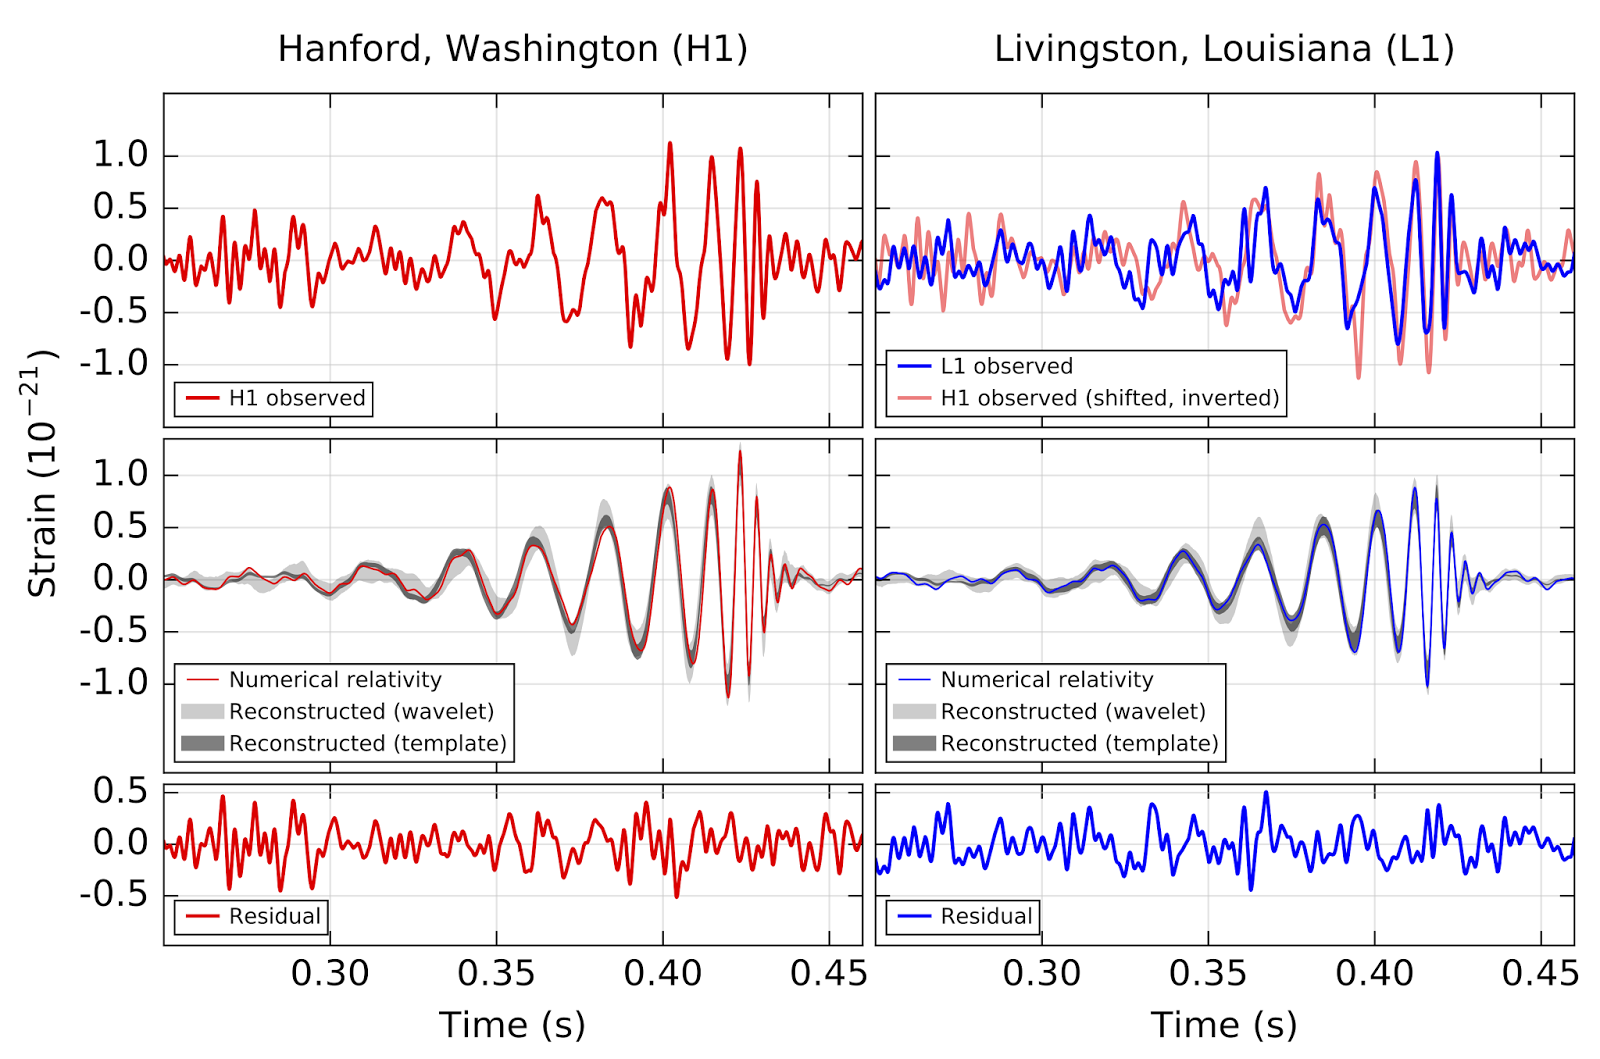
\includegraphics[width=0.4\textwidth]{figs/Fig1_Split_v17_top3_standalone.png} \hfill
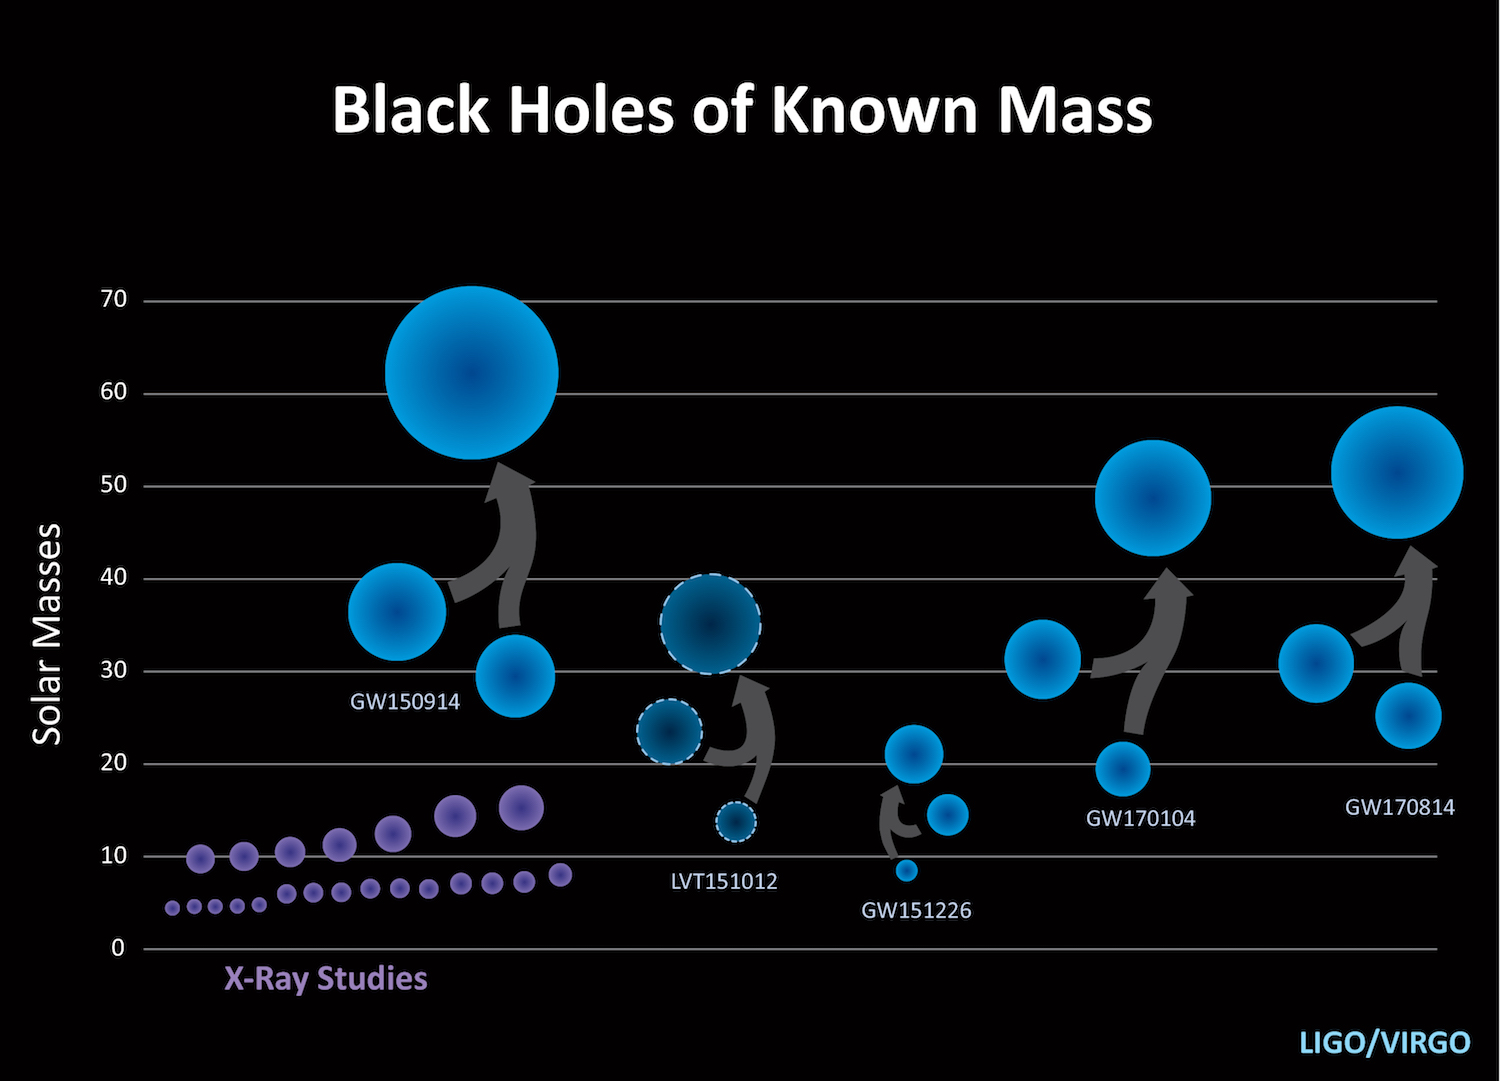
\includegraphics[width=0.4\textwidth]{figs/BHmassChartGW170814-sm.jpg}
\caption{\small image credit: \url{https://www.ligo.org/detections.php}}
\end{figure}

\begin{itemize}
	\item In $2015$ the first GW detection by LIGO \& VIRGO has revolutionized multimessenger astronomy.
	\item Numerical simulations to construct GW forms are essential
	\item Current detections have been for roughly equal mass ratio
\end{itemize}

\end{frame}

\begin{frame}{Challenges in Computational General Relativity}
\begin{itemize}
	\item Existing frameworks \textcolor{blue}{lack scalability} and \textcolor{blue}{unable to handle large mass ratios}.
	\item Complexity of Einstein equations (especially numerical formulation of GR field equations)
	\item Known numerical methods only uses \textcolor{blue}{Finite Difference(FD)} approximations with time evolution
	\item Since number of grid points $ \propto q^3$ efficient \textbf{adaptivity} is needed to handle $q\geq 10$
\end{itemize}
\end{frame}

\begin{frame}{Contributions}
\begin{itemize}
	\item \textbf{Wavelet Adaptive Multi-Resolution(WAMR)}: Existing approaches uses, structured or block adaptivity which makes the $q\geq 10$ challenging/ not feasible to run. \textit{WAMR is the key component which makes $q\geq 10$ cases possible in \textsc{Dendro-GR}}.
	\item \textbf{\tsearch}: Neighborhood information is essential for FD computations, we present $\mathcal{O}(klog(n))$ approach for fast search operations on adaptive octrees. 
	\item \textbf{Symbolic optimized code generation}: Computing differential operators $D_x,\mathcal{L}_\beta$ can be challenging on curved manifolds(spacetime). Automatic code generation also improves the code portability on different architectures(OpenMp,AVX,CUDA). 
	\item \textbf{Scalability}: We present scalabilty upto 131k cores of \Titan~ on mass ratios upto 100.
\end{itemize}
\end{frame}


\begin{frame}{Wavelet Adaptive Multi-Resolution(WAMR)}
\onslide<1->
{
\begin{figure}
	\centering
	\resizebox{0.9\textwidth}{!}{
	\begin{tikzpicture}[yscale=-1.0]
	\begin{scope}[yshift=5]
	\foreach \y in {0,1,2}
	\node[text width=1cm] at (-1,\y) {\small $V_\y$};
	\foreach \x in {0,4,8,12,16}
	\fill (\x,0) circle (0.1cm);
	
	\foreach \x in {0,2,4,6,8,10,12,14,16}
	\fill (\x,1) circle (0.1cm);		
	
	\foreach \x in {0,1,2,3,4,5,6,7,8,9,10,11,12,13,14,15,16}
	\fill (\x,2) circle (0.1cm);
	
	\node[text width=10cm,align=center] at (8,3.5) {\subcaption{$f(x) \in V_0 \subset V_1 \subset V_2$ \label{fig:w:a}} };
	\end{scope}
	\end{tikzpicture}
}
\end{figure}
}	


\onslide<2>
{
	\begin{figure}
		\centering
		\resizebox{0.9\textwidth}{!}{
			\begin{tikzpicture}[yscale=-1.0]
			\begin{scope}[yshift=0cm]
				\foreach \y in {1,2}
			\node[text width=1cm] at (-1,\y) {\small $W_\y$};
			\foreach \x in {0,4,8,12,16}
			\fill (\x,0) circle (0.1cm);
			
			\foreach \x in {2,6,10,14}
			\fill[red] (\x,1) circle (0.1cm);		
			
			\foreach \x in {1,3,5,7,9,11,13,15}
			\fill[blue] (\x,2) circle (0.1cm);
			
			\node[text width=15cm,align=center] at (8,3.5) {\subcaption{$W_{i,k}=|f(V_{i,k})-I(f(V{i-1,:}))|$ \label{fig:w:b}}};
			\end{scope}
			\node[text width=1cm] at (-1,0) {\small $V_0$};
			\end{tikzpicture}
		}
	\end{figure}
}	


\end{frame}

\begin{frame}{Wavelet Adaptive Multi-Resolution(WAMR)}
\onslide<1->
{
	\begin{figure}
			\resizebox{0.9\textwidth}{!}{
		\begin{tikzpicture}[yscale=-1.0]
	   	\begin{scope}[yshift=0cm]
			\node[text width=1cm] at (-1,0) {\small $V_0$};
			
			\foreach \y in {1,2}
			\node[text width=1cm] at (-1,\y) {\small $W_\y$};
			\foreach \x in {0,4,8,12,16}
			\fill (\x,0) circle (0.1cm);
			
			\foreach \x in {2,6,10,14}
			\fill[red] (\x,1) circle (0.1cm);		
			
			\draw[red] (6,1) circle (0.2cm);
			\draw[red] (10,1) circle (0.2cm);
			
			\foreach \x in {1,3,5,7,9,11,13,15}
			\fill[blue] (\x,2) circle (0.1cm);
			
			\draw[blue] (1,2) circle (0.2cm);
			\draw[blue] (3,2) circle (0.2cm);
			\draw[blue] (13,2) circle (0.2cm);
			\draw[blue] (15,2) circle (0.2cm);
			
			\node[text width=15cm,align=center] at (8,3.5) {\subcaption{$W_{i,k}\geq \epsilon \geq 0$ \label{fig:w:c}}};
			
			\end{scope}
		\end{tikzpicture}
	}
	\end{figure}
}

\onslide<2>
{
	\begin{figure}
		\resizebox{0.9\textwidth}{!}{
			\begin{tikzpicture}[yscale=-1.0]
			\begin{scope}[yshift=0cm]
			\node[text width=1cm] at (-1,0) {\small $V_0$};
		
		\foreach \y in {1,2}
		\node[text width=1cm] at (-1,\y) {\small $W_\y$};
		\foreach \x in {0,4,8,12,16}
		\fill (\x,0) circle (0.1cm);
		
		%	\foreach \x in {2,6,10,14}z
		%	\fill[red] (\x,1) circle (0.1cm);		
		
		\draw[red] (6,1) circle (0.2cm);
		\draw[red] (10,1) circle (0.2cm);
		
		%	\foreach \x in {1,3,5,7,9,11,13,15}
		%	\fill[blue] (\x,2) circle (0.1cm);
		
		\draw[blue] (1,2) circle (0.2cm);
		\draw[blue] (3,2) circle (0.2cm);
		\draw[blue] (13,2) circle (0.2cm);
		\draw[blue] (15,2) circle (0.2cm);
		
		\node[text width=15cm,align=center] at (8,3.5) {\subcaption{wavelet/sparse representation of $f(x)$ \label{fig:w:d}}};
			
			\end{scope}
			\end{tikzpicture}
		}
	\end{figure}
}
\end{frame}


\begin{frame}{\tsearch: Efficient search operations on Octrees}
\begin{figure}
	\centering
	\resizebox{0.9\textwidth}{!}{
		\begin{tikzpicture}[scale=1.5, every node/.style={scale=2.5}]
		
		% \draw[gray, very thin] (0,0) grid +(8,8);
		\onslide<1->{
		
		\begin{scope}[shift={(0,0)}]
		\draw[thick] (0,0) rectangle +(8,8);
		\draw[step=4,thick] (0,0) grid +(8,8);
		\draw[step=2,thick] (0,4) grid +(4,4);
		\draw[step=2,thick] (4,0) grid +(4,4);
		\draw[step=1,thick] (2,6) grid +(2,2);
		
		\draw[fill=red!60] (3.8,7.7) rectangle +(0.2,0.2);
		\node at (4.5,7.0) {\small $k_1$};
		\draw[fill=red!60] (6,6) rectangle +(0.2,0.2);
		\node at (6,5.5) {\small $k_2$};
		\draw[fill=red!60] (7,3) rectangle +(0.2,0.2);
		\node at (7,2.5) {\small $k_3$};
		\draw[fill=red!60] (2,2) rectangle +(0.2,0.2);
		\node at (2.0,1.5) {\small $k_4$};
		\draw[fill=red!60] (3,3) rectangle +(0.2,0.2);
		\node at (3.0,2.5) {\small $k_5$};
		
		\end{scope}	 	
	}
		\onslide<2->{
		\begin{scope}[shift={(11,0)}]
		\draw[thick] (0,0) rectangle +(8,8);
		\draw[step=4,cpu4,thick] (0,0) grid +(8,8);
		
		\node at (0.5,0.5) {\small $1$};
		\node at (4.5,0.5) {\small $4$};
		\node at (0.5,4.5) {\small $7$};
		\node at (4.5,4.5) {\small $1$};
		
		\draw[fill=red!60] (3.8,7.7) rectangle +(0.2,0.2);
		\node at (4.5,7.0) {\small $k_1$};
		\draw[fill=red!60] (6,6) rectangle +(0.2,0.2);
		\node at (6,5.5) {\small $k_2$};
		\draw[fill=red!60] (7,3) rectangle +(0.2,0.2);
		\node at (7,2.5) {\small $k_3$};
		\draw[fill=red!60] (2,2) rectangle +(0.2,0.2);
		\node at (2.0,1.5) {\small $k_4$};
		\draw[fill=red!60] (3,3) rectangle +(0.2,0.2);
		\node at (3.0,2.5) {\small $k_5$};
		
		\end{scope}
		}	
	\onslide<3->{
		\begin{scope}[shift={(22,0)}]
		\draw[thick] (0,0) rectangle +(8,8);
		\draw[step=4,cpu4,thick] (0,0) grid +(8,8);
		\draw[step=2,cpu3,thick] (0,4) grid +(4,4);
		\draw[step=2,cpu3,thick] (4,0) grid +(4,4);
		\node at (0.5,0.5) {\small $1$};
		
		\node at (4.5,0.5) {\small $1$};
		\node at (6.5,0.5) {\small $1$};
		\node at (4.5,2.5) {\small $1$};
		\node at (6.5,2.5) {\small $1$};
		
		\node at (0.5,4.5) {\small $1$};
		\node at (2.5,4.5) {\small $1$};
		\node at (0.5,6.5) {\small $1$};
		\node at (2.5,6.5) {\small $4$};
		
		\node at (4.5,4.5) {\small $1$};	
		
		\draw[fill=red!60] (3.8,7.7) rectangle +(0.2,0.2);
		\node at (4.5,7.0) {\small $k_1$};
		\draw[fill=red!60] (6,6) rectangle +(0.2,0.2);
		\node at (6,5.5) {\small $k_2$};
		\draw[fill=red!60] (7,3) rectangle +(0.2,0.2);
		\node at (7.5,2.5) {\small $k_3$};
		\draw[fill=red!60] (2,2) rectangle +(0.2,0.2);
		\node at (2.0,1.5) {\small $k_4$};
		\draw[fill=red!60] (3,3) rectangle +(0.2,0.2);
		\node at (3.0,2.5) {\small $k_5$};
		\end{scope}
	}
			\onslide<4->{
		\begin{scope}[shift={(33,0)}]
		\draw[thick] (0,0) rectangle +(8,8);
		\draw[step=4,cpu4,thick] (0,0) grid +(8,8);
		\draw[step=2,cpu3,thick] (0,4) grid +(4,4);
		\draw[step=2,cpu3,thick] (4,0) grid +(4,4);
		\draw[step=1,cpu1,thick] (2,6) grid +(2,2);
		
		\node at (0.5,0.5) {\small $1$};
		
		\node at (4.5,0.5) {\small $1$};
		\node at (6.5,0.5) {\small $1$};
		\node at (4.5,2.5) {\small $1$};
		\node at (6.5,2.5) {\small $1$};
		
		\node at (0.5,4.5) {\small $1$};
		\node at (2.5,4.5) {\small $1$};
		\node at (0.5,6.5) {\small $1$};
		
		\node at (2.5,6.5) {\small $1$};
		\node at (3.5,6.5) {\small $1$};
		\node at (2.5,7.5) {\small $1$};
		\node at (3.5,7.5) {\small $1$};
		
		\node at (4.5,4.5) {\small $1$};		
		
		
		\draw[fill=red!60] (3.8,7.7) rectangle +(0.2,0.2);
		\node at (4.5,7.0) {\small $k_1$};
		\draw[fill=red!60] (6,6) rectangle +(0.2,0.2);
		\node at (6,5.5) {\small $k_2$};
		\draw[fill=red!60] (7,3) rectangle +(0.2,0.2);
		\node at (7.5,2.5) {\small $k_3$};
		\draw[fill=red!60] (2,2) rectangle +(0.2,0.2);
		\node at (2.0,1.5) {\small $k_4$};
		\draw[fill=red!60] (3,3) rectangle +(0.2,0.2);
		\node at (3.0,2.5) {\small $k_5$};
		
		\end{scope}
	}
		\end{tikzpicture}
	}
\end{figure}

\end{frame}

\begin{frame}{\tsearch: Efficient search operations on Octrees}
\begin{figure}
	\centering
	\begin{tikzpicture}
	\begin{axis}[legend pos= north west,xlabel={number of keys $\rightarrow$},symbolic x coords={100,1K,10K,100K,1M,10M,20M,33M,64M},
	xtick={data},
	ylabel={time(s) $\rightarrow$},grid=major,width=10cm,height=5cm,
	x tick label style={font=\tiny}]
	\addplot [sq_b1,thin,mark=*]table [x={numKeys},y={bsearch_time_s}]{dat/stampede2/tsearch.dat};
	\addplot [sq_r1,thin,mark=x] table [x={numKeys},y={tsearch_time_s}]{dat/stampede2/tsearch.dat};
	\legend{\texttt{std::bsearch}, \tsearch }
	\end{axis}
	\end{tikzpicture}
	\caption{Comparison of \texttt{std::bsearch} with operator $<$ and comparison free \tsearch~ approach for performing, varying number of keys on $33M$ sorted octree in \Stampede~ \texttt{SKX} node.}
	\label{fig::balcomparison}
\end{figure}
\end{frame}

\begin{frame}[fragile]{Symbolic Code Generation}
\vspace{-0.5in}
\begin{figure}
	%	 \noindent\fbox{
	%	\onslide<1->{
	\begin{minipage}[t]{.48\textwidth}
		\footnotesize
		\begin{eqnarray*}
			\partial_t \alpha &=&  \mathcal{L}_\beta\alpha - 2 \alpha K, \\
			\partial_t \beta^i &=& \lambda_2 \beta^j\,\partial_j\beta^i + \frac{3}{4} f(\alpha) B^i\\
			\partial_t B^i  &=& \partial_t \tilde\Gamma^i  - \eta B^{i}   + \lambda_3 \beta^j\,\partial_j B^i - \lambda_4 \beta^j\,\partial_j \tilde\Gamma^i \\
			\partial_t \tilde \gamma_{ij} &=&  \mathcal{L}_\beta\tilde{\gamma}_{ij} -2 \alpha \tilde A_{ij}, \\
			\partial_t \chi &=& \mathcal{L}_\beta\chi + \frac{2}{3}\chi \left(\alpha K -  
			\partial_a \beta^a\right)\\
			\partial_t \tilde A_{ij} &=& \mathcal{L}_\beta\tilde{A}_{ij} + \chi \left(-D_i D_j \alpha +
			\alpha R_{ij}\right)^{TF} +\nonumber \\
			&\,&\alpha \left(K \tilde A_{ij} -
			2 \tilde A_{ik} \tilde A^{k}_{\,j}\right), \label{eq:at_evol}\\
			\partial_t K &=& \beta^k\partial_kK- D^i D_i \alpha + \\
			&\,&\alpha \left(\tilde A_{ij}\tilde
			A^{ij} +\frac{1}{3}K^2\right),\\
			\partial_t \tilde \Gamma^i &=& \tilde \gamma^{jk} \partial_j
			\partial_k \beta^i + \frac{1}{3} \tilde \gamma^{ij} \partial_j
			\partial_k \beta^k + \beta^j \partial_j \tilde \Gamma^i - \nonumber \\
			&\,&\tilde
			\Gamma^j \partial_j \beta^i + 
			\frac{2}{3}\tilde \Gamma^i \partial_j
			\beta^j - 2 \tilde A^{i j}\partial_j \alpha + \nonumber \\
			&\,& 2 \alpha \left(\tilde
			{\Gamma^i}_{jk} \tilde A^{jk} - \frac{2}{3 \chi} \tilde A^{ij}\partial_j \chi -
			\frac{2}{3} \tilde \gamma^{ij} \partial_j K\right) \\
			% ~ &~ & ~\\
		\end{eqnarray*}
	\end{minipage}\hfill% This must go next to `\end{minipage}`
\end{figure}
\end{frame}

\begin{frame}[fragile]{Symbolic Code Generation}
\vspace{-0.5in}
	\begin{figure}
	%	 \noindent\fbox{
%	\onslide<1->{
	\begin{minipage}[t]{.48\textwidth}
		\footnotesize
		\begin{eqnarray*}
			\partial_t \alpha &=&  \mathcal{L}_\beta\alpha - 2 \alpha K, \\
			\partial_t \beta^i &=& \lambda_2 \beta^j\,\partial_j\beta^i + \frac{3}{4} f(\alpha) B^i\\
			\partial_t B^i  &=& \partial_t \tilde\Gamma^i  - \eta B^{i}   + \lambda_3 \beta^j\,\partial_j B^i - \lambda_4 \beta^j\,\partial_j \tilde\Gamma^i \\
			\partial_t \tilde \gamma_{ij} &=&  \mathcal{L}_\beta\tilde{\gamma}_{ij} -2 \alpha \tilde A_{ij}, \\
			\partial_t \chi &=& \mathcal{L}_\beta\chi + \frac{2}{3}\chi \left(\alpha K -  
			\partial_a \beta^a\right)\\
			\partial_t \tilde A_{ij} &=& \mathcal{L}_\beta\tilde{A}_{ij} + \chi \left(-D_i D_j \alpha +
			\alpha R_{ij}\right)^{TF} +\nonumber \\
			&\,&\alpha \left(K \tilde A_{ij} -
			2 \tilde A_{ik} \tilde A^{k}_{\,j}\right), \label{eq:at_evol}\\
			\partial_t K &=& \beta^k\partial_kK- D^i D_i \alpha + \\
			&\,&\alpha \left(\tilde A_{ij}\tilde
			A^{ij} +\frac{1}{3}K^2\right),\\
			\partial_t \tilde \Gamma^i &=& \tilde \gamma^{jk} \partial_j
			\partial_k \beta^i + \frac{1}{3} \tilde \gamma^{ij} \partial_j
			\partial_k \beta^k + \beta^j \partial_j \tilde \Gamma^i - \nonumber \\
			&\,&\tilde
			\Gamma^j \partial_j \beta^i + 
			\frac{2}{3}\tilde \Gamma^i \partial_j
			\beta^j - 2 \tilde A^{i j}\partial_j \alpha + \nonumber \\
			&\,& 2 \alpha \left(\tilde
			{\Gamma^i}_{jk} \tilde A^{jk} - \frac{2}{3 \chi} \tilde A^{ij}\partial_j \chi -
			\frac{2}{3} \tilde \gamma^{ij} \partial_j K\right) \\
			% ~ &~ & ~\\
		\end{eqnarray*}
	\end{minipage}\hfill% This must go next to `\end{minipage}`
	%		}
%}
%\onslide<2>{
%\vspace{-0.1in}
	\begin{minipage}[t]{.52\textwidth}
		\footnotesize
		%frame=single,framesep=1pt,
		\begin{minted}[frame=single,framesep=1pt,bgcolor=yellow!10]{python}
			
 from DENDRO_sym import *
 a_rhs = Dendro.Lie(b, a) - 2*a*K
 b_rhs = [3/4 * f(a) * B[i] + 
 l2*vec_j_del_j(b, b[i]) for i in e_i]
 l2*vec_j_del_j(b, b[i]) 
 for i in e_i]
 B_rhs = [Gt_rhs[i] - eta * B[i] + 
 l3 * vec_j_del_j(b, B[i]) - 
 l4 * vec_j_del_j(b, Gt[i]) 
 for i in e_i]
 gt_rhs =  Dendro.Lie(b, gt) - 2*a*At
 chi_rhs = Dendro.Lie(b, chi) + 
 2/3*chi*(a*K - del_j(b)) 
 At_rhs = Dendro.Lie(b, At) + chi *
 Dendro.TF(-DiDj(a) + 
 a*Dendro.Ricci) +
 a*(K*At -2*At_ikAtKj)
 K_rhs = vec_k_del_k(K) - DIDi(a) +
 a*(1/3*K*K + A_ij_A_IJ(At)) 
\end{minted}
	\end{minipage}
%}
	%\caption{\label{fig:symb} \small The left panel shows the \BSSN ~formulation of the Einstein equations. These are tensor equations, with indices $i,j,\ldots$ taking the values $1, 2, 3$. On the right we show the \texttt{{\dendro\_sym}} code for these equations. \texttt{\dendro\_sym} uses \texttt{SymPy} and other tools to generate optimized C++ code to evaluate the equations. Note that $\mathcal{L}_\beta,\ D,\ \partial$ denote Lie derivative, covariant derivative and partial derivative respectively, and we have excluded $\partial_t\Gamma^i$ from \texttt{\dendro\_sym} to save space.}
	%\label{fig:bssneqs}
	\vspace{-0.15in}
\end{figure}
\end{frame}

\begin{frame}{FD computations on adaptive octrees}
\begin{figure}
	\centering
	\resizebox{0.9\textwidth}{!}{
		\begin{tikzpicture}[scale=0.2,every node/.style={scale=0.6}]
		\path [blue,fill=cyan,line width=0.5mm,bend left,->,every node/.style={black,sloped,anchor=south,auto=false}] (5,12) edge node{\textit{\ \tiny unzip}} (35,14);
		\path [blue,fill=cyan,line width=0.5mm,bend left,->,every node/.style={black,sloped,anchor=south,auto=false}] (35,0) edge node{\textit{\ \tiny zip}} (5,-2);
		\begin{scope}[shift={(0,0)}]
		\draw[step=5cm] (0,0) grid +(10,10);
		\draw[step=2.5cm] (5,0) grid +(5,5);
		\draw[step=2.5cm] (0,5) grid +(5,5);
		
		\def \r{0.12}
		\foreach \x in {0,2.5,5}{
			\foreach \y in {0,2.5,5}{
				\draw[red,fill=red] (\x,\y) circle (\r);
			}
		}
		
		\foreach \x in {5,7.5,10}{
			\foreach \y in {5,7.5,10}{
				\draw[red,fill=red] (\x,\y) circle (\r);
			}
		}
		
		\foreach \x in {0,1.25,2.5,3.75}{
			\foreach \y in {6.25,7.5,8.75,10}{
				\draw[blue,fill=blue] (\x,\y) circle (\r);
			}
		}	
		
		\foreach \x in {6.25,7.5,8.75,10}{
			\foreach \y in {0,1.25,2.5,3.75}{
				\draw[blue,fill=blue] (\x,\y) circle (\r);
			}
		}
		\end{scope}
		
		\begin{scope}[shift={(14,0)}]
		%\draw[cyan,thick,fill=blue!20] (-1,-1) rectangle +(6,6);
		\draw[cyan,thick] (0,0) rectangle +(5,5);
		\draw[cyan,thick,xshift=2cm,yshift=2.0cm] (5,5) rectangle +(5,5);
		\draw[cyan,thick,step=2.5cm,xshift=2.0cm] (5,0) grid +(5,5);
		\draw[cyan,thick,step=2.5cm,yshift=2.0cm] (0,5) grid +(5,5);
		%	\draw[cyan,thick] (0,4) rectangle +(2,2);
		%	\draw[cyan,thick] (2,4) rectangle +(2,2);
		%	\draw[cyan,thick] (2,6) rectangle +(2,2);
		%	\draw[cyan,thick] (4,0) rectangle +(2,2);
		%	\draw[cyan,thick] (6,2) rectangle +(2,2);
		%	\draw[cyan,thick] (6,0) rectangle +(2,2);
		\end{scope}
		
		\begin{scope}[shift={(30,0)}]
		\def \r{0.12}
		\draw[cyan,fill=blue!50,fill opacity=0.5]
		(-2,-2)--(-2,6)--(6,6)--(6,-2)--cycle
		(0,0) -- (4,0)-- (4,4)--(0,4)--cycle;
		\foreach \x in {-2,0,2,2,4,6}{
			\foreach \y in {-2,0,2,2,4,6}{
				\draw[red,fill=red] (\x,\y) circle (\r);
			}
		}
		
		\draw[cyan,thick,fill=blue!50,fill opacity=0.5,even odd rule,xshift=8.5cm,yshift=8.5cm] 
		(-2,-2)--(-2,6)--(6,6)--(6,-2)--cycle
		(0,0) -- (4,0)-- (4,4)--(0,4)--cycle;
		\foreach \x in {-2,0,2,2,4,6}{
			\foreach \y in {-2,0,2,2,4,6}{
				\draw[red,fill=red,xshift=8.5cm,yshift=8.5cm] (\x,\y) circle (\r);
			}
		}
		
		\draw[cyan,thick,fill=blue!50,fill opacity=0.5,even odd rule,xshift=8.5cm] 
		(-1,-1)--(-1,5)--(5,5)--(5,-1)--cycle
		(0,0) -- (4,0)-- (4,4)--(0,4)--cycle;
		\draw[cyan,thick,step=2,xshift=8.5cm] (0,0) grid +(4,4);
		\foreach \x in {-1,0,1,2,3,4,5}{
			\foreach \y in {-1,0,1,2,3,4,5}{
				\draw[blue,fill=blue,xshift=8.5cm] (\x,\y) circle (\r);
			}
		}
		
		\draw[cyan,thick,fill=blue!50,fill opacity=0.5,even odd rule,yshift=8.5cm] 
		(-1,-1)--(-1,5)--(5,5)--(5,-1)--cycle
		(0,0) -- (4,0)-- (4,4)--(0,4)--cycle;
		\draw[cyan,thick,step=2,yshift=8.5cm] (0,0) grid +(4,4);	
		\foreach \x in {-1,0,1,2,3,4,5}{
			\foreach \y in {-1,0,1,2,3,4,5}{
				\draw[blue,fill=blue,yshift=8.5cm] (\x,\y) circle (\r);
			}
		}
		
		\end{scope}	
		\end{tikzpicture}
	}	
%	\caption{\label{fig:unzip} A simplistic example of octree to block decomposition and \unzip~ operation. The leftmost figure shows the considering adaptive octree with \cgn~ and its block decomposition is shown in the middle. Note that the given octree is decomposed into four regular blocks of different sizes. The rightmost figure shows the decomposed blocks padded with values coming from neighboring octants with interpolation if needed. In order to perform \unzip~ operation both $\psi$ and $\psi$ mappings are used. }
%	\vspace{-0.15in}
\end{figure}

\end{frame}

\begin{frame}{Overview}
\begin{figure}
	%\centering
	\resizebox{0.98\textwidth}{!}{
		\begin{tikzpicture}
		\def\xmax{18}
		\def\xmin{0}
		\def\ymin{0}
		\def\ymax{6}
		\begin{scope}
		%\draw[very thin,step=1] (\xmin,\ymin) grid +(\xmax,\ymax);
		%\draw[blue,thin,fill=yellow!20,fill opacity=0.7] (\xmin,\ymax-2) rectangle +(1.5,1.8) node[black,pos=.5,align=center] {\small parameter \\ file};
		\draw[->,thick] (\xmin+0.2,3) -- (\xmin+1.5,3);
		\node[text width=2cm] at (\xmin+1.25,3.5) {initial $u_0$};
		\draw[line width=0.5mm,->] (\xmin+2,\ymax+1) -- (\xmax-1,\ymax+1) node[anchor=south east] {$t$};
		\end{scope}
		\begin{scope}[xshift=2cm,yshift=2.5cm]
		\node[anchor=south west,inner sep=0] at (0,0) {
\includegraphics[width=2cm]{figs/gr_init1_r1.png}};
		\end{scope}
		%\begin{scope}[xshift=2cm,yshift=0.25cm]
		%\node[anchor=south west,inner sep=0] at (0,0) {\includegraphics[width=2cm]{figs/gr_init_r1.png}};
		%\end{scope}0.0078
		\begin{scope}[xshift=2cm,yshift=0.25cm,scale=0.03]
		\draw [gray, ultra thin] (0.000000, 64.000000) rectangle +(8.000000,-8.000000);
\draw [gray, ultra thin] (8.000000, 64.000000) rectangle +(8.000000,-8.000000);
\draw [gray, ultra thin] (16.000000, 64.000000) rectangle +(8.000000,-8.000000);
\draw [gray, ultra thin] (24.000000, 64.000000) rectangle +(8.000000,-8.000000);
\draw [gray, ultra thin] (32.000000, 64.000000) rectangle +(8.000000,-8.000000);
\draw [gray, ultra thin] (40.000000, 64.000000) rectangle +(8.000000,-8.000000);
\draw [gray, ultra thin] (48.000000, 64.000000) rectangle +(8.000000,-8.000000);
\draw [gray, ultra thin] (56.000000, 64.000000) rectangle +(8.000000,-8.000000);
\draw [gray, ultra thin] (0.000000, 56.000000) rectangle +(8.000000,-8.000000);
\draw [gray, ultra thin] (8.000000, 56.000000) rectangle +(4.000000,-4.000000);
\draw [gray, ultra thin] (12.000000, 56.000000) rectangle +(4.000000,-4.000000);
\draw [gray, ultra thin] (16.000000, 56.000000) rectangle +(4.000000,-4.000000);
\draw [gray, ultra thin] (20.000000, 56.000000) rectangle +(4.000000,-4.000000);
\draw [gray, ultra thin] (24.000000, 56.000000) rectangle +(4.000000,-4.000000);
\draw [gray, ultra thin] (28.000000, 56.000000) rectangle +(4.000000,-4.000000);
\draw [gray, ultra thin] (32.000000, 56.000000) rectangle +(4.000000,-4.000000);
\draw [gray, ultra thin] (36.000000, 56.000000) rectangle +(4.000000,-4.000000);
\draw [gray, ultra thin] (40.000000, 56.000000) rectangle +(4.000000,-4.000000);
\draw [gray, ultra thin] (44.000000, 56.000000) rectangle +(4.000000,-4.000000);
\draw [gray, ultra thin] (48.000000, 56.000000) rectangle +(4.000000,-4.000000);
\draw [gray, ultra thin] (52.000000, 56.000000) rectangle +(4.000000,-4.000000);
\draw [gray, ultra thin] (56.000000, 56.000000) rectangle +(8.000000,-8.000000);
\draw [gray, ultra thin] (8.000000, 52.000000) rectangle +(4.000000,-4.000000);
\draw [gray, ultra thin] (12.000000, 52.000000) rectangle +(4.000000,-4.000000);
\draw [gray, ultra thin] (16.000000, 52.000000) rectangle +(4.000000,-4.000000);
\draw [gray, ultra thin] (20.000000, 52.000000) rectangle +(4.000000,-4.000000);
\draw [gray, ultra thin] (24.000000, 52.000000) rectangle +(4.000000,-4.000000);
\draw [gray, ultra thin] (28.000000, 52.000000) rectangle +(4.000000,-4.000000);
\draw [gray, ultra thin] (32.000000, 52.000000) rectangle +(4.000000,-4.000000);
\draw [gray, ultra thin] (36.000000, 52.000000) rectangle +(4.000000,-4.000000);
\draw [gray, ultra thin] (40.000000, 52.000000) rectangle +(4.000000,-4.000000);
\draw [gray, ultra thin] (44.000000, 52.000000) rectangle +(4.000000,-4.000000);
\draw [gray, ultra thin] (48.000000, 52.000000) rectangle +(4.000000,-4.000000);
\draw [gray, ultra thin] (52.000000, 52.000000) rectangle +(4.000000,-4.000000);
\draw [gray, ultra thin] (0.000000, 48.000000) rectangle +(4.000000,-4.000000);
\draw [gray, ultra thin] (4.000000, 48.000000) rectangle +(4.000000,-4.000000);
\draw [gray, ultra thin] (8.000000, 48.000000) rectangle +(4.000000,-4.000000);
\draw [gray, ultra thin] (12.000000, 48.000000) rectangle +(4.000000,-4.000000);
\draw [gray, ultra thin] (16.000000, 48.000000) rectangle +(4.000000,-4.000000);
\draw [gray, ultra thin] (20.000000, 48.000000) rectangle +(2.000000,-2.000000);
\draw [gray, ultra thin] (22.000000, 48.000000) rectangle +(2.000000,-2.000000);
\draw [gray, ultra thin] (24.000000, 48.000000) rectangle +(4.000000,-4.000000);
\draw [gray, ultra thin] (28.000000, 48.000000) rectangle +(4.000000,-4.000000);
\draw [gray, ultra thin] (32.000000, 48.000000) rectangle +(4.000000,-4.000000);
\draw [gray, ultra thin] (36.000000, 48.000000) rectangle +(4.000000,-4.000000);
\draw [gray, ultra thin] (40.000000, 48.000000) rectangle +(2.000000,-2.000000);
\draw [gray, ultra thin] (42.000000, 48.000000) rectangle +(2.000000,-2.000000);
\draw [gray, ultra thin] (44.000000, 48.000000) rectangle +(4.000000,-4.000000);
\draw [gray, ultra thin] (48.000000, 48.000000) rectangle +(4.000000,-4.000000);
\draw [gray, ultra thin] (52.000000, 48.000000) rectangle +(4.000000,-4.000000);
\draw [gray, ultra thin] (56.000000, 48.000000) rectangle +(4.000000,-4.000000);
\draw [gray, ultra thin] (60.000000, 48.000000) rectangle +(4.000000,-4.000000);
\draw [gray, ultra thin] (20.000000, 46.000000) rectangle +(2.000000,-2.000000);
\draw [gray, ultra thin] (22.000000, 46.000000) rectangle +(2.000000,-2.000000);
\draw [gray, ultra thin] (40.000000, 46.000000) rectangle +(2.000000,-2.000000);
\draw [gray, ultra thin] (42.000000, 46.000000) rectangle +(2.000000,-2.000000);
\draw [gray, ultra thin] (0.000000, 44.000000) rectangle +(4.000000,-4.000000);
\draw [gray, ultra thin] (4.000000, 44.000000) rectangle +(4.000000,-4.000000);
\draw [gray, ultra thin] (8.000000, 44.000000) rectangle +(4.000000,-4.000000);
\draw [gray, ultra thin] (12.000000, 44.000000) rectangle +(2.000000,-2.000000);
\draw [gray, ultra thin] (14.000000, 44.000000) rectangle +(2.000000,-2.000000);
\draw [gray, ultra thin] (16.000000, 44.000000) rectangle +(2.000000,-2.000000);
\draw [gray, ultra thin] (18.000000, 44.000000) rectangle +(2.000000,-2.000000);
\draw [gray, ultra thin] (20.000000, 44.000000) rectangle +(2.000000,-2.000000);
\draw [gray, ultra thin] (22.000000, 44.000000) rectangle +(2.000000,-2.000000);
\draw [gray, ultra thin] (24.000000, 44.000000) rectangle +(2.000000,-2.000000);
\draw [gray, ultra thin] (26.000000, 44.000000) rectangle +(2.000000,-2.000000);
\draw [gray, ultra thin] (28.000000, 44.000000) rectangle +(4.000000,-4.000000);
\draw [gray, ultra thin] (32.000000, 44.000000) rectangle +(4.000000,-4.000000);
\draw [gray, ultra thin] (36.000000, 44.000000) rectangle +(2.000000,-2.000000);
\draw [gray, ultra thin] (38.000000, 44.000000) rectangle +(2.000000,-2.000000);
\draw [gray, ultra thin] (40.000000, 44.000000) rectangle +(2.000000,-2.000000);
\draw [gray, ultra thin] (42.000000, 44.000000) rectangle +(2.000000,-2.000000);
\draw [gray, ultra thin] (44.000000, 44.000000) rectangle +(2.000000,-2.000000);
\draw [gray, ultra thin] (46.000000, 44.000000) rectangle +(2.000000,-2.000000);
\draw [gray, ultra thin] (48.000000, 44.000000) rectangle +(2.000000,-2.000000);
\draw [gray, ultra thin] (50.000000, 44.000000) rectangle +(2.000000,-2.000000);
\draw [gray, ultra thin] (52.000000, 44.000000) rectangle +(4.000000,-4.000000);
\draw [gray, ultra thin] (56.000000, 44.000000) rectangle +(4.000000,-4.000000);
\draw [gray, ultra thin] (60.000000, 44.000000) rectangle +(4.000000,-4.000000);
\draw [gray, ultra thin] (12.000000, 42.000000) rectangle +(2.000000,-2.000000);
\draw [gray, ultra thin] (14.000000, 42.000000) rectangle +(2.000000,-2.000000);
\draw [gray, ultra thin] (16.000000, 42.000000) rectangle +(2.000000,-2.000000);
\draw [gray, ultra thin] (18.000000, 42.000000) rectangle +(2.000000,-2.000000);
\draw [gray, ultra thin] (20.000000, 42.000000) rectangle +(2.000000,-2.000000);
\draw [gray, ultra thin] (22.000000, 42.000000) rectangle +(2.000000,-2.000000);
\draw [gray, ultra thin] (24.000000, 42.000000) rectangle +(2.000000,-2.000000);
\draw [gray, ultra thin] (26.000000, 42.000000) rectangle +(2.000000,-2.000000);
\draw [gray, ultra thin] (36.000000, 42.000000) rectangle +(2.000000,-2.000000);
\draw [gray, ultra thin] (38.000000, 42.000000) rectangle +(2.000000,-2.000000);
\draw [gray, ultra thin] (40.000000, 42.000000) rectangle +(2.000000,-2.000000);
\draw [gray, ultra thin] (42.000000, 42.000000) rectangle +(2.000000,-2.000000);
\draw [gray, ultra thin] (44.000000, 42.000000) rectangle +(2.000000,-2.000000);
\draw [gray, ultra thin] (46.000000, 42.000000) rectangle +(2.000000,-2.000000);
\draw [gray, ultra thin] (48.000000, 42.000000) rectangle +(2.000000,-2.000000);
\draw [gray, ultra thin] (50.000000, 42.000000) rectangle +(2.000000,-2.000000);
\draw [gray, ultra thin] (0.000000, 40.000000) rectangle +(8.000000,-8.000000);
\draw [gray, ultra thin] (8.000000, 40.000000) rectangle +(4.000000,-4.000000);
\draw [gray, ultra thin] (12.000000, 40.000000) rectangle +(2.000000,-2.000000);
\draw [gray, ultra thin] (14.000000, 40.000000) rectangle +(2.000000,-2.000000);
\draw [gray, ultra thin] (16.000000, 40.000000) rectangle +(2.000000,-2.000000);
\draw [gray, ultra thin] (18.000000, 40.000000) rectangle +(2.000000,-2.000000);
\draw [gray, ultra thin] (20.000000, 40.000000) rectangle +(2.000000,-2.000000);
\draw [gray, ultra thin] (22.000000, 40.000000) rectangle +(2.000000,-2.000000);
\draw [gray, ultra thin] (24.000000, 40.000000) rectangle +(2.000000,-2.000000);
\draw [gray, ultra thin] (26.000000, 40.000000) rectangle +(2.000000,-2.000000);
\draw [gray, ultra thin] (28.000000, 40.000000) rectangle +(2.000000,-2.000000);
\draw [gray, ultra thin] (30.000000, 40.000000) rectangle +(2.000000,-2.000000);
\draw [gray, ultra thin] (32.000000, 40.000000) rectangle +(2.000000,-2.000000);
\draw [gray, ultra thin] (34.000000, 40.000000) rectangle +(2.000000,-2.000000);
\draw [gray, ultra thin] (36.000000, 40.000000) rectangle +(2.000000,-2.000000);
\draw [gray, ultra thin] (38.000000, 40.000000) rectangle +(2.000000,-2.000000);
\draw [gray, ultra thin] (40.000000, 40.000000) rectangle +(2.000000,-2.000000);
\draw [gray, ultra thin] (42.000000, 40.000000) rectangle +(2.000000,-2.000000);
\draw [gray, ultra thin] (44.000000, 40.000000) rectangle +(2.000000,-2.000000);
\draw [gray, ultra thin] (46.000000, 40.000000) rectangle +(2.000000,-2.000000);
\draw [gray, ultra thin] (48.000000, 40.000000) rectangle +(2.000000,-2.000000);
\draw [gray, ultra thin] (50.000000, 40.000000) rectangle +(2.000000,-2.000000);
\draw [gray, ultra thin] (52.000000, 40.000000) rectangle +(4.000000,-4.000000);
\draw [gray, ultra thin] (56.000000, 40.000000) rectangle +(4.000000,-4.000000);
\draw [gray, ultra thin] (60.000000, 40.000000) rectangle +(4.000000,-4.000000);
\draw [gray, ultra thin] (12.000000, 38.000000) rectangle +(2.000000,-2.000000);
\draw [gray, ultra thin] (14.000000, 38.000000) rectangle +(2.000000,-2.000000);
\draw [gray, ultra thin] (16.000000, 38.000000) rectangle +(2.000000,-2.000000);
\draw [gray, ultra thin] (18.000000, 38.000000) rectangle +(1.000000,-1.000000);
\draw [gray, ultra thin] (19.000000, 38.000000) rectangle +(1.000000,-1.000000);
\draw [gray, ultra thin] (20.000000, 38.000000) rectangle +(1.000000,-1.000000);
\draw [gray, ultra thin] (21.000000, 38.000000) rectangle +(1.000000,-1.000000);
\draw [gray, ultra thin] (22.000000, 38.000000) rectangle +(1.000000,-1.000000);
\draw [gray, ultra thin] (23.000000, 38.000000) rectangle +(1.000000,-1.000000);
\draw [gray, ultra thin] (24.000000, 38.000000) rectangle +(2.000000,-2.000000);
\draw [gray, ultra thin] (26.000000, 38.000000) rectangle +(2.000000,-2.000000);
\draw [gray, ultra thin] (28.000000, 38.000000) rectangle +(2.000000,-2.000000);
\draw [gray, ultra thin] (30.000000, 38.000000) rectangle +(2.000000,-2.000000);
\draw [gray, ultra thin] (32.000000, 38.000000) rectangle +(2.000000,-2.000000);
\draw [gray, ultra thin] (34.000000, 38.000000) rectangle +(2.000000,-2.000000);
\draw [gray, ultra thin] (36.000000, 38.000000) rectangle +(2.000000,-2.000000);
\draw [gray, ultra thin] (38.000000, 38.000000) rectangle +(2.000000,-2.000000);
\draw [gray, ultra thin] (40.000000, 38.000000) rectangle +(1.000000,-1.000000);
\draw [gray, ultra thin] (41.000000, 38.000000) rectangle +(1.000000,-1.000000);
\draw [gray, ultra thin] (42.000000, 38.000000) rectangle +(1.000000,-1.000000);
\draw [gray, ultra thin] (43.000000, 38.000000) rectangle +(1.000000,-1.000000);
\draw [gray, ultra thin] (44.000000, 38.000000) rectangle +(2.000000,-2.000000);
\draw [gray, ultra thin] (46.000000, 38.000000) rectangle +(2.000000,-2.000000);
\draw [gray, ultra thin] (48.000000, 38.000000) rectangle +(2.000000,-2.000000);
\draw [gray, ultra thin] (50.000000, 38.000000) rectangle +(2.000000,-2.000000);
\draw [gray, ultra thin] (18.000000, 37.000000) rectangle +(1.000000,-1.000000);
\draw [gray, ultra thin] (19.000000, 37.000000) rectangle +(1.000000,-1.000000);
\draw [gray, ultra thin] (20.000000, 37.000000) rectangle +(1.000000,-1.000000);
\draw [gray, ultra thin] (21.000000, 37.000000) rectangle +(1.000000,-1.000000);
\draw [gray, ultra thin] (22.000000, 37.000000) rectangle +(1.000000,-1.000000);
\draw [gray, ultra thin] (23.000000, 37.000000) rectangle +(1.000000,-1.000000);
\draw [gray, ultra thin] (40.000000, 37.000000) rectangle +(1.000000,-1.000000);
\draw [gray, ultra thin] (41.000000, 37.000000) rectangle +(1.000000,-1.000000);
\draw [gray, ultra thin] (42.000000, 37.000000) rectangle +(1.000000,-1.000000);
\draw [gray, ultra thin] (43.000000, 37.000000) rectangle +(1.000000,-1.000000);
\draw [gray, ultra thin] (8.000000, 36.000000) rectangle +(4.000000,-4.000000);
\draw [gray, ultra thin] (12.000000, 36.000000) rectangle +(2.000000,-2.000000);
\draw [gray, ultra thin] (14.000000, 36.000000) rectangle +(2.000000,-2.000000);
\draw [gray, ultra thin] (16.000000, 36.000000) rectangle +(1.000000,-1.000000);
\draw [gray, ultra thin] (17.000000, 36.000000) rectangle +(1.000000,-1.000000);
\draw [gray, ultra thin] (18.000000, 36.000000) rectangle +(1.000000,-1.000000);
\draw [gray, ultra thin] (19.000000, 36.000000) rectangle +(1.000000,-1.000000);
\draw [gray, ultra thin] (20.000000, 36.000000) rectangle +(1.000000,-1.000000);
\draw [gray, ultra thin] (21.000000, 36.000000) rectangle +(1.000000,-1.000000);
\draw [gray, ultra thin] (22.000000, 36.000000) rectangle +(2.000000,-2.000000);
\draw [gray, ultra thin] (24.000000, 36.000000) rectangle +(2.000000,-2.000000);
\draw [gray, ultra thin] (26.000000, 36.000000) rectangle +(2.000000,-2.000000);
\draw [gray, ultra thin] (28.000000, 36.000000) rectangle +(2.000000,-2.000000);
\draw [gray, ultra thin] (30.000000, 36.000000) rectangle +(2.000000,-2.000000);
\draw [gray, ultra thin] (32.000000, 36.000000) rectangle +(2.000000,-2.000000);
\draw [gray, ultra thin] (34.000000, 36.000000) rectangle +(2.000000,-2.000000);
\draw [gray, ultra thin] (36.000000, 36.000000) rectangle +(2.000000,-2.000000);
\draw [gray, ultra thin] (38.000000, 36.000000) rectangle +(2.000000,-2.000000);
\draw [gray, ultra thin] (40.000000, 36.000000) rectangle +(2.000000,-2.000000);
\draw [gray, ultra thin] (42.000000, 36.000000) rectangle +(1.000000,-1.000000);
\draw [gray, ultra thin] (43.000000, 36.000000) rectangle +(1.000000,-1.000000);
\draw [gray, ultra thin] (44.000000, 36.000000) rectangle +(1.000000,-1.000000);
\draw [gray, ultra thin] (45.000000, 36.000000) rectangle +(1.000000,-1.000000);
\draw [gray, ultra thin] (46.000000, 36.000000) rectangle +(2.000000,-2.000000);
\draw [gray, ultra thin] (48.000000, 36.000000) rectangle +(2.000000,-2.000000);
\draw [gray, ultra thin] (50.000000, 36.000000) rectangle +(2.000000,-2.000000);
\draw [gray, ultra thin] (52.000000, 36.000000) rectangle +(4.000000,-4.000000);
\draw [gray, ultra thin] (56.000000, 36.000000) rectangle +(4.000000,-4.000000);
\draw [gray, ultra thin] (60.000000, 36.000000) rectangle +(4.000000,-4.000000);
\draw [gray, ultra thin] (16.000000, 35.000000) rectangle +(1.000000,-1.000000);
\draw [gray, ultra thin] (17.000000, 35.000000) rectangle +(1.000000,-1.000000);
\draw [gray, ultra thin] (18.000000, 35.000000) rectangle +(1.000000,-1.000000);
\draw [gray, ultra thin] (19.000000, 35.000000) rectangle +(1.000000,-1.000000);
\draw [gray, ultra thin] (20.000000, 35.000000) rectangle +(1.000000,-1.000000);
\draw [gray, ultra thin] (21.000000, 35.000000) rectangle +(1.000000,-1.000000);
\draw [gray, ultra thin] (42.000000, 35.000000) rectangle +(1.000000,-1.000000);
\draw [gray, ultra thin] (43.000000, 35.000000) rectangle +(1.000000,-1.000000);
\draw [gray, ultra thin] (44.000000, 35.000000) rectangle +(1.000000,-1.000000);
\draw [gray, ultra thin] (45.000000, 35.000000) rectangle +(1.000000,-1.000000);
\draw [gray, ultra thin] (12.000000, 34.000000) rectangle +(2.000000,-2.000000);
\draw [gray, ultra thin] (14.000000, 34.000000) rectangle +(2.000000,-2.000000);
\draw [gray, ultra thin] (16.000000, 34.000000) rectangle +(2.000000,-2.000000);
\draw [gray, ultra thin] (18.000000, 34.000000) rectangle +(1.000000,-1.000000);
\draw [gray, ultra thin] (19.000000, 34.000000) rectangle +(1.000000,-1.000000);
\draw [gray, ultra thin] (20.000000, 34.000000) rectangle +(2.000000,-2.000000);
\draw [gray, ultra thin] (22.000000, 34.000000) rectangle +(0.500000,-0.500000);
\draw [gray, ultra thin] (22.500000, 34.000000) rectangle +(0.500000,-0.500000);
\draw [gray, ultra thin] (23.000000, 34.000000) rectangle +(0.500000,-0.500000);
\draw [gray, ultra thin] (23.500000, 34.000000) rectangle +(0.500000,-0.500000);
\draw [gray, ultra thin] (24.000000, 34.000000) rectangle +(0.500000,-0.500000);
\draw [gray, ultra thin] (24.500000, 34.000000) rectangle +(0.500000,-0.500000);
\draw [gray, ultra thin] (25.000000, 34.000000) rectangle +(0.500000,-0.500000);
\draw [gray, ultra thin] (25.500000, 34.000000) rectangle +(0.500000,-0.500000);
\draw [gray, ultra thin] (26.000000, 34.000000) rectangle +(2.000000,-2.000000);
\draw [gray, ultra thin] (28.000000, 34.000000) rectangle +(2.000000,-2.000000);
\draw [gray, ultra thin] (30.000000, 34.000000) rectangle +(2.000000,-2.000000);
\draw [gray, ultra thin] (32.000000, 34.000000) rectangle +(2.000000,-2.000000);
\draw [gray, ultra thin] (34.000000, 34.000000) rectangle +(2.000000,-2.000000);
\draw [gray, ultra thin] (36.000000, 34.000000) rectangle +(1.000000,-1.000000);
\draw [gray, ultra thin] (37.000000, 34.000000) rectangle +(1.000000,-1.000000);
\draw [gray, ultra thin] (38.000000, 34.000000) rectangle +(0.500000,-0.500000);
\draw [gray, ultra thin] (38.500000, 34.000000) rectangle +(0.500000,-0.500000);
\draw [gray, ultra thin] (39.000000, 34.000000) rectangle +(0.500000,-0.500000);
\draw [gray, ultra thin] (39.500000, 34.000000) rectangle +(0.500000,-0.500000);
\draw [gray, ultra thin] (40.000000, 34.000000) rectangle +(0.500000,-0.500000);
\draw [gray, ultra thin] (40.500000, 34.000000) rectangle +(0.500000,-0.500000);
\draw [gray, ultra thin] (41.000000, 34.000000) rectangle +(1.000000,-1.000000);
\draw [gray, ultra thin] (42.000000, 34.000000) rectangle +(2.000000,-2.000000);
\draw [gray, ultra thin] (44.000000, 34.000000) rectangle +(1.000000,-1.000000);
\draw [gray, ultra thin] (45.000000, 34.000000) rectangle +(1.000000,-1.000000);
\draw [gray, ultra thin] (46.000000, 34.000000) rectangle +(2.000000,-2.000000);
\draw [gray, ultra thin] (48.000000, 34.000000) rectangle +(2.000000,-2.000000);
\draw [gray, ultra thin] (50.000000, 34.000000) rectangle +(2.000000,-2.000000);
\draw [gray, ultra thin] (22.000000, 33.500000) rectangle +(0.500000,-0.500000);
\draw [gray, ultra thin] (22.500000, 33.500000) rectangle +(0.500000,-0.500000);
\draw [gray, ultra thin] (23.000000, 33.500000) rectangle +(0.250000,-0.250000);
\draw [gray, ultra thin] (23.250000, 33.500000) rectangle +(0.250000,-0.250000);
\draw [gray, ultra thin] (23.500000, 33.500000) rectangle +(0.250000,-0.250000);
\draw [gray, ultra thin] (23.750000, 33.500000) rectangle +(0.250000,-0.250000);
\draw [gray, ultra thin] (24.000000, 33.500000) rectangle +(0.500000,-0.500000);
\draw [gray, ultra thin] (24.500000, 33.500000) rectangle +(0.250000,-0.250000);
\draw [gray, ultra thin] (24.750000, 33.500000) rectangle +(0.250000,-0.250000);
\draw [gray, ultra thin] (25.000000, 33.500000) rectangle +(0.500000,-0.500000);
\draw [gray, ultra thin] (25.500000, 33.500000) rectangle +(0.500000,-0.500000);
\draw [gray, ultra thin] (38.000000, 33.500000) rectangle +(0.500000,-0.500000);
\draw [gray, ultra thin] (38.500000, 33.500000) rectangle +(0.500000,-0.500000);
\draw [gray, ultra thin] (39.000000, 33.500000) rectangle +(0.500000,-0.500000);
\draw [gray, ultra thin] (39.500000, 33.500000) rectangle +(0.250000,-0.250000);
\draw [gray, ultra thin] (39.750000, 33.500000) rectangle +(0.250000,-0.250000);
\draw [gray, ultra thin] (40.000000, 33.500000) rectangle +(0.250000,-0.250000);
\draw [gray, ultra thin] (40.250000, 33.500000) rectangle +(0.250000,-0.250000);
\draw [gray, ultra thin] (40.500000, 33.500000) rectangle +(0.500000,-0.500000);
\draw [gray, ultra thin] (23.000000, 33.250000) rectangle +(0.250000,-0.250000);
\draw [gray, ultra thin] (23.250000, 33.250000) rectangle +(0.250000,-0.250000);
\draw [gray, ultra thin] (23.500000, 33.250000) rectangle +(0.250000,-0.250000);
\draw [gray, ultra thin] (23.750000, 33.250000) rectangle +(0.250000,-0.250000);
\draw [gray, ultra thin] (24.500000, 33.250000) rectangle +(0.250000,-0.250000);
\draw [gray, ultra thin] (24.750000, 33.250000) rectangle +(0.250000,-0.250000);
\draw [gray, ultra thin] (39.500000, 33.250000) rectangle +(0.250000,-0.250000);
\draw [gray, ultra thin] (39.750000, 33.250000) rectangle +(0.250000,-0.250000);
\draw [gray, ultra thin] (40.000000, 33.250000) rectangle +(0.250000,-0.250000);
\draw [gray, ultra thin] (40.250000, 33.250000) rectangle +(0.250000,-0.250000);
\draw [gray, ultra thin] (18.000000, 33.000000) rectangle +(1.000000,-1.000000);
\draw [gray, ultra thin] (19.000000, 33.000000) rectangle +(1.000000,-1.000000);
\draw [gray, ultra thin] (22.000000, 33.000000) rectangle +(0.500000,-0.500000);
\draw [gray, ultra thin] (22.500000, 33.000000) rectangle +(0.250000,-0.250000);
\draw [gray, ultra thin] (22.750000, 33.000000) rectangle +(0.250000,-0.250000);
\draw [gray, ultra thin] (23.000000, 33.000000) rectangle +(0.250000,-0.250000);
\draw [gray, ultra thin] (23.250000, 33.000000) rectangle +(0.250000,-0.250000);
\draw [gray, ultra thin] (23.500000, 33.000000) rectangle +(0.250000,-0.250000);
\draw [gray, ultra thin] (23.750000, 33.000000) rectangle +(0.250000,-0.250000);
\draw [gray, ultra thin] (24.000000, 33.000000) rectangle +(0.250000,-0.250000);
\draw [gray, ultra thin] (24.250000, 33.000000) rectangle +(0.250000,-0.250000);
\draw [gray, ultra thin] (24.500000, 33.000000) rectangle +(0.250000,-0.250000);
\draw [gray, ultra thin] (24.750000, 33.000000) rectangle +(0.250000,-0.250000);
\draw [gray, ultra thin] (25.000000, 33.000000) rectangle +(0.250000,-0.250000);
\draw [gray, ultra thin] (25.250000, 33.000000) rectangle +(0.250000,-0.250000);
\draw [gray, ultra thin] (25.500000, 33.000000) rectangle +(0.500000,-0.500000);
\draw [gray, ultra thin] (36.000000, 33.000000) rectangle +(1.000000,-1.000000);
\draw [gray, ultra thin] (37.000000, 33.000000) rectangle +(0.500000,-0.500000);
\draw [gray, ultra thin] (37.500000, 33.000000) rectangle +(0.500000,-0.500000);
\draw [gray, ultra thin] (38.000000, 33.000000) rectangle +(0.250000,-0.250000);
\draw [gray, ultra thin] (38.250000, 33.000000) rectangle +(0.250000,-0.250000);
\draw [gray, ultra thin] (38.500000, 33.000000) rectangle +(0.250000,-0.250000);
\draw [gray, ultra thin] (38.750000, 33.000000) rectangle +(0.250000,-0.250000);
\draw [gray, ultra thin] (39.000000, 33.000000) rectangle +(0.250000,-0.250000);
\draw [gray, ultra thin] (39.250000, 33.000000) rectangle +(0.250000,-0.250000);
\draw [gray, ultra thin] (39.500000, 33.000000) rectangle +(0.250000,-0.250000);
\draw [gray, ultra thin] (39.750000, 33.000000) rectangle +(0.250000,-0.250000);
\draw [gray, ultra thin] (40.000000, 33.000000) rectangle +(0.250000,-0.250000);
\draw [gray, ultra thin] (40.250000, 33.000000) rectangle +(0.250000,-0.250000);
\draw [gray, ultra thin] (40.500000, 33.000000) rectangle +(0.250000,-0.250000);
\draw [gray, ultra thin] (40.750000, 33.000000) rectangle +(0.250000,-0.250000);
\draw [gray, ultra thin] (41.000000, 33.000000) rectangle +(0.500000,-0.500000);
\draw [gray, ultra thin] (41.500000, 33.000000) rectangle +(0.500000,-0.500000);
\draw [gray, ultra thin] (44.000000, 33.000000) rectangle +(1.000000,-1.000000);
\draw [gray, ultra thin] (45.000000, 33.000000) rectangle +(1.000000,-1.000000);
\draw [gray, ultra thin] (22.500000, 32.750000) rectangle +(0.250000,-0.250000);
\draw [gray, ultra thin] (22.750000, 32.750000) rectangle +(0.250000,-0.250000);
\draw [gray, ultra thin] (23.000000, 32.750000) rectangle +(0.250000,-0.250000);
\draw [gray, ultra thin] (23.250000, 32.750000) rectangle +(0.250000,-0.250000);
\draw [gray, ultra thin] (23.500000, 32.750000) rectangle +(0.250000,-0.250000);
\draw [gray, ultra thin] (23.750000, 32.750000) rectangle +(0.250000,-0.250000);
\draw [gray, ultra thin] (24.000000, 32.750000) rectangle +(0.250000,-0.250000);
\draw [gray, ultra thin] (24.250000, 32.750000) rectangle +(0.250000,-0.250000);
\draw [gray, ultra thin] (24.500000, 32.750000) rectangle +(0.250000,-0.250000);
\draw [gray, ultra thin] (24.750000, 32.750000) rectangle +(0.250000,-0.250000);
\draw [gray, ultra thin] (25.000000, 32.750000) rectangle +(0.250000,-0.250000);
\draw [gray, ultra thin] (25.250000, 32.750000) rectangle +(0.250000,-0.250000);
\draw [gray, ultra thin] (38.000000, 32.750000) rectangle +(0.250000,-0.250000);
\draw [gray, ultra thin] (38.250000, 32.750000) rectangle +(0.250000,-0.250000);
\draw [gray, ultra thin] (38.500000, 32.750000) rectangle +(0.250000,-0.250000);
\draw [gray, ultra thin] (38.750000, 32.750000) rectangle +(0.250000,-0.250000);
\draw [gray, ultra thin] (39.000000, 32.750000) rectangle +(0.250000,-0.250000);
\draw [gray, ultra thin] (39.250000, 32.750000) rectangle +(0.250000,-0.250000);
\draw [gray, ultra thin] (39.500000, 32.750000) rectangle +(0.250000,-0.250000);
\draw [gray, ultra thin] (39.750000, 32.750000) rectangle +(0.250000,-0.250000);
\draw [gray, ultra thin] (40.000000, 32.750000) rectangle +(0.250000,-0.250000);
\draw [gray, ultra thin] (40.250000, 32.750000) rectangle +(0.250000,-0.250000);
\draw [gray, ultra thin] (40.500000, 32.750000) rectangle +(0.250000,-0.250000);
\draw [gray, ultra thin] (40.750000, 32.750000) rectangle +(0.250000,-0.250000);
\draw [gray, ultra thin] (22.000000, 32.500000) rectangle +(0.500000,-0.500000);
\draw [gray, ultra thin] (22.500000, 32.500000) rectangle +(0.250000,-0.250000);
\draw [gray, ultra thin] (22.750000, 32.500000) rectangle +(0.250000,-0.250000);
\draw [gray, ultra thin] (23.000000, 32.500000) rectangle +(0.250000,-0.250000);
\draw [gray, ultra thin] (23.250000, 32.500000) rectangle +(0.250000,-0.250000);
\draw [gray, ultra thin] (23.500000, 32.500000) rectangle +(0.250000,-0.250000);
\draw [gray, ultra thin] (23.750000, 32.500000) rectangle +(0.250000,-0.250000);
\draw [gray, ultra thin] (24.000000, 32.500000) rectangle +(0.250000,-0.250000);
\draw [gray, ultra thin] (24.250000, 32.500000) rectangle +(0.250000,-0.250000);
\draw [gray, ultra thin] (24.500000, 32.500000) rectangle +(0.250000,-0.250000);
\draw [gray, ultra thin] (24.750000, 32.500000) rectangle +(0.250000,-0.250000);
\draw [gray, ultra thin] (25.000000, 32.500000) rectangle +(0.250000,-0.250000);
\draw [gray, ultra thin] (25.250000, 32.500000) rectangle +(0.250000,-0.250000);
\draw [gray, ultra thin] (25.500000, 32.500000) rectangle +(0.500000,-0.500000);
\draw [gray, ultra thin] (37.000000, 32.500000) rectangle +(0.500000,-0.500000);
\draw [gray, ultra thin] (37.500000, 32.500000) rectangle +(0.500000,-0.500000);
\draw [gray, ultra thin] (38.000000, 32.500000) rectangle +(0.250000,-0.250000);
\draw [gray, ultra thin] (38.250000, 32.500000) rectangle +(0.250000,-0.250000);
\draw [gray, ultra thin] (38.500000, 32.500000) rectangle +(0.250000,-0.250000);
\draw [gray, ultra thin] (38.750000, 32.500000) rectangle +(0.250000,-0.250000);
\draw [gray, ultra thin] (39.000000, 32.500000) rectangle +(0.250000,-0.250000);
\draw [gray, ultra thin] (39.250000, 32.500000) rectangle +(0.250000,-0.250000);
\draw [gray, ultra thin] (39.500000, 32.500000) rectangle +(0.250000,-0.250000);
\draw [gray, ultra thin] (39.750000, 32.500000) rectangle +(0.250000,-0.250000);
\draw [gray, ultra thin] (40.000000, 32.500000) rectangle +(0.250000,-0.250000);
\draw [gray, ultra thin] (40.250000, 32.500000) rectangle +(0.250000,-0.250000);
\draw [gray, ultra thin] (40.500000, 32.500000) rectangle +(0.250000,-0.250000);
\draw [gray, ultra thin] (40.750000, 32.500000) rectangle +(0.250000,-0.250000);
\draw [gray, ultra thin] (41.000000, 32.500000) rectangle +(0.500000,-0.500000);
\draw [gray, ultra thin] (41.500000, 32.500000) rectangle +(0.500000,-0.500000);
\draw [gray, ultra thin] (22.500000, 32.250000) rectangle +(0.250000,-0.250000);
\draw [gray, ultra thin] (22.750000, 32.250000) rectangle +(0.250000,-0.250000);
\draw [gray, ultra thin] (23.000000, 32.250000) rectangle +(0.250000,-0.250000);
\draw [gray, ultra thin] (23.250000, 32.250000) rectangle +(0.250000,-0.250000);
\draw [gray, ultra thin] (23.500000, 32.250000) rectangle +(0.125000,-0.125000);
\draw [gray, ultra thin] (23.625000, 32.250000) rectangle +(0.125000,-0.125000);
\draw [gray, ultra thin] (23.750000, 32.250000) rectangle +(0.250000,-0.250000);
\draw [gray, ultra thin] (24.000000, 32.250000) rectangle +(0.250000,-0.250000);
\draw [gray, ultra thin] (24.250000, 32.250000) rectangle +(0.125000,-0.125000);
\draw [gray, ultra thin] (24.375000, 32.250000) rectangle +(0.125000,-0.125000);
\draw [gray, ultra thin] (24.500000, 32.250000) rectangle +(0.250000,-0.250000);
\draw [gray, ultra thin] (24.750000, 32.250000) rectangle +(0.250000,-0.250000);
\draw [gray, ultra thin] (25.000000, 32.250000) rectangle +(0.250000,-0.250000);
\draw [gray, ultra thin] (25.250000, 32.250000) rectangle +(0.250000,-0.250000);
\draw [gray, ultra thin] (38.000000, 32.250000) rectangle +(0.250000,-0.250000);
\draw [gray, ultra thin] (38.250000, 32.250000) rectangle +(0.250000,-0.250000);
\draw [gray, ultra thin] (38.500000, 32.250000) rectangle +(0.250000,-0.250000);
\draw [gray, ultra thin] (38.750000, 32.250000) rectangle +(0.250000,-0.250000);
\draw [gray, ultra thin] (39.000000, 32.250000) rectangle +(0.125000,-0.125000);
\draw [gray, ultra thin] (39.125000, 32.250000) rectangle +(0.125000,-0.125000);
\draw [gray, ultra thin] (39.250000, 32.250000) rectangle +(0.250000,-0.250000);
\draw [gray, ultra thin] (39.500000, 32.250000) rectangle +(0.250000,-0.250000);
\draw [gray, ultra thin] (39.750000, 32.250000) rectangle +(0.125000,-0.125000);
\draw [gray, ultra thin] (39.875000, 32.250000) rectangle +(0.125000,-0.125000);
\draw [gray, ultra thin] (40.000000, 32.250000) rectangle +(0.250000,-0.250000);
\draw [gray, ultra thin] (40.250000, 32.250000) rectangle +(0.250000,-0.250000);
\draw [gray, ultra thin] (40.500000, 32.250000) rectangle +(0.250000,-0.250000);
\draw [gray, ultra thin] (40.750000, 32.250000) rectangle +(0.250000,-0.250000);
\draw [gray, ultra thin] (23.500000, 32.125000) rectangle +(0.125000,-0.125000);
\draw [gray, ultra thin] (23.625000, 32.125000) rectangle +(0.125000,-0.125000);
\draw [gray, ultra thin] (24.250000, 32.125000) rectangle +(0.125000,-0.125000);
\draw [gray, ultra thin] (24.375000, 32.125000) rectangle +(0.125000,-0.125000);
\draw [gray, ultra thin] (39.000000, 32.125000) rectangle +(0.125000,-0.125000);
\draw [gray, ultra thin] (39.125000, 32.125000) rectangle +(0.125000,-0.125000);
\draw [gray, ultra thin] (39.750000, 32.125000) rectangle +(0.125000,-0.125000);
\draw [gray, ultra thin] (39.875000, 32.125000) rectangle +(0.125000,-0.125000);
\draw [gray, ultra thin] (0.000000, 32.000000) rectangle +(8.000000,-8.000000);
\draw [gray, ultra thin] (8.000000, 32.000000) rectangle +(4.000000,-4.000000);
\draw [gray, ultra thin] (12.000000, 32.000000) rectangle +(2.000000,-2.000000);
\draw [gray, ultra thin] (14.000000, 32.000000) rectangle +(2.000000,-2.000000);
\draw [gray, ultra thin] (16.000000, 32.000000) rectangle +(2.000000,-2.000000);
\draw [gray, ultra thin] (18.000000, 32.000000) rectangle +(1.000000,-1.000000);
\draw [gray, ultra thin] (19.000000, 32.000000) rectangle +(1.000000,-1.000000);
\draw [gray, ultra thin] (20.000000, 32.000000) rectangle +(2.000000,-2.000000);
\draw [gray, ultra thin] (22.000000, 32.000000) rectangle +(0.500000,-0.500000);
\draw [gray, ultra thin] (22.500000, 32.000000) rectangle +(0.250000,-0.250000);
\draw [gray, ultra thin] (22.750000, 32.000000) rectangle +(0.250000,-0.250000);
\draw [gray, ultra thin] (23.000000, 32.000000) rectangle +(0.250000,-0.250000);
\draw [gray, ultra thin] (23.250000, 32.000000) rectangle +(0.125000,-0.125000);
\draw [gray, ultra thin] (23.375000, 32.000000) rectangle +(0.125000,-0.125000);
\draw [gray, ultra thin] (23.500000, 32.000000) rectangle +(0.250000,-0.250000);
\draw [gray, ultra thin] (23.750000, 32.000000) rectangle +(0.250000,-0.250000);
\draw [gray, ultra thin] (24.000000, 32.000000) rectangle +(0.250000,-0.250000);
\draw [gray, ultra thin] (24.250000, 32.000000) rectangle +(0.125000,-0.125000);
\draw [gray, ultra thin] (24.375000, 32.000000) rectangle +(0.125000,-0.125000);
\draw [gray, ultra thin] (24.500000, 32.000000) rectangle +(0.250000,-0.250000);
\draw [gray, ultra thin] (24.750000, 32.000000) rectangle +(0.250000,-0.250000);
\draw [gray, ultra thin] (25.000000, 32.000000) rectangle +(0.250000,-0.250000);
\draw [gray, ultra thin] (25.250000, 32.000000) rectangle +(0.250000,-0.250000);
\draw [gray, ultra thin] (25.500000, 32.000000) rectangle +(0.500000,-0.500000);
\draw [gray, ultra thin] (26.000000, 32.000000) rectangle +(2.000000,-2.000000);
\draw [gray, ultra thin] (28.000000, 32.000000) rectangle +(4.000000,-4.000000);
\draw [gray, ultra thin] (32.000000, 32.000000) rectangle +(4.000000,-4.000000);
\draw [gray, ultra thin] (36.000000, 32.000000) rectangle +(1.000000,-1.000000);
\draw [gray, ultra thin] (37.000000, 32.000000) rectangle +(0.500000,-0.500000);
\draw [gray, ultra thin] (37.500000, 32.000000) rectangle +(0.500000,-0.500000);
\draw [gray, ultra thin] (38.000000, 32.000000) rectangle +(0.250000,-0.250000);
\draw [gray, ultra thin] (38.250000, 32.000000) rectangle +(0.250000,-0.250000);
\draw [gray, ultra thin] (38.500000, 32.000000) rectangle +(0.250000,-0.250000);
\draw [gray, ultra thin] (38.750000, 32.000000) rectangle +(0.250000,-0.250000);
\draw [gray, ultra thin] (39.000000, 32.000000) rectangle +(0.125000,-0.125000);
\draw [gray, ultra thin] (39.125000, 32.000000) rectangle +(0.125000,-0.125000);
\draw [gray, ultra thin] (39.250000, 32.000000) rectangle +(0.250000,-0.250000);
\draw [gray, ultra thin] (39.500000, 32.000000) rectangle +(0.250000,-0.250000);
\draw [gray, ultra thin] (39.750000, 32.000000) rectangle +(0.250000,-0.250000);
\draw [gray, ultra thin] (40.000000, 32.000000) rectangle +(0.250000,-0.250000);
\draw [gray, ultra thin] (40.250000, 32.000000) rectangle +(0.250000,-0.250000);
\draw [gray, ultra thin] (40.500000, 32.000000) rectangle +(0.250000,-0.250000);
\draw [gray, ultra thin] (40.750000, 32.000000) rectangle +(0.250000,-0.250000);
\draw [gray, ultra thin] (41.000000, 32.000000) rectangle +(0.500000,-0.500000);
\draw [gray, ultra thin] (41.500000, 32.000000) rectangle +(0.500000,-0.500000);
\draw [gray, ultra thin] (42.000000, 32.000000) rectangle +(2.000000,-2.000000);
\draw [gray, ultra thin] (44.000000, 32.000000) rectangle +(1.000000,-1.000000);
\draw [gray, ultra thin] (45.000000, 32.000000) rectangle +(1.000000,-1.000000);
\draw [gray, ultra thin] (46.000000, 32.000000) rectangle +(2.000000,-2.000000);
\draw [gray, ultra thin] (48.000000, 32.000000) rectangle +(2.000000,-2.000000);
\draw [gray, ultra thin] (50.000000, 32.000000) rectangle +(2.000000,-2.000000);
\draw [gray, ultra thin] (52.000000, 32.000000) rectangle +(4.000000,-4.000000);
\draw [gray, ultra thin] (56.000000, 32.000000) rectangle +(4.000000,-4.000000);
\draw [gray, ultra thin] (60.000000, 32.000000) rectangle +(4.000000,-4.000000);
\draw [gray, ultra thin] (23.250000, 31.875000) rectangle +(0.125000,-0.125000);
\draw [gray, ultra thin] (23.375000, 31.875000) rectangle +(0.125000,-0.125000);
\draw [gray, ultra thin] (24.250000, 31.875000) rectangle +(0.125000,-0.125000);
\draw [gray, ultra thin] (24.375000, 31.875000) rectangle +(0.125000,-0.125000);
\draw [gray, ultra thin] (39.000000, 31.875000) rectangle +(0.125000,-0.125000);
\draw [gray, ultra thin] (39.125000, 31.875000) rectangle +(0.125000,-0.125000);
\draw [gray, ultra thin] (22.500000, 31.750000) rectangle +(0.250000,-0.250000);
\draw [gray, ultra thin] (22.750000, 31.750000) rectangle +(0.250000,-0.250000);
\draw [gray, ultra thin] (23.000000, 31.750000) rectangle +(0.250000,-0.250000);
\draw [gray, ultra thin] (23.250000, 31.750000) rectangle +(0.250000,-0.250000);
\draw [gray, ultra thin] (23.500000, 31.750000) rectangle +(0.250000,-0.250000);
\draw [gray, ultra thin] (23.750000, 31.750000) rectangle +(0.250000,-0.250000);
\draw [gray, ultra thin] (24.000000, 31.750000) rectangle +(0.250000,-0.250000);
\draw [gray, ultra thin] (24.250000, 31.750000) rectangle +(0.250000,-0.250000);
\draw [gray, ultra thin] (24.500000, 31.750000) rectangle +(0.250000,-0.250000);
\draw [gray, ultra thin] (24.750000, 31.750000) rectangle +(0.250000,-0.250000);
\draw [gray, ultra thin] (25.000000, 31.750000) rectangle +(0.250000,-0.250000);
\draw [gray, ultra thin] (25.250000, 31.750000) rectangle +(0.250000,-0.250000);
\draw [gray, ultra thin] (38.000000, 31.750000) rectangle +(0.250000,-0.250000);
\draw [gray, ultra thin] (38.250000, 31.750000) rectangle +(0.250000,-0.250000);
\draw [gray, ultra thin] (38.500000, 31.750000) rectangle +(0.250000,-0.250000);
\draw [gray, ultra thin] (38.750000, 31.750000) rectangle +(0.250000,-0.250000);
\draw [gray, ultra thin] (39.000000, 31.750000) rectangle +(0.250000,-0.250000);
\draw [gray, ultra thin] (39.250000, 31.750000) rectangle +(0.250000,-0.250000);
\draw [gray, ultra thin] (39.500000, 31.750000) rectangle +(0.250000,-0.250000);
\draw [gray, ultra thin] (39.750000, 31.750000) rectangle +(0.250000,-0.250000);
\draw [gray, ultra thin] (40.000000, 31.750000) rectangle +(0.250000,-0.250000);
\draw [gray, ultra thin] (40.250000, 31.750000) rectangle +(0.250000,-0.250000);
\draw [gray, ultra thin] (40.500000, 31.750000) rectangle +(0.250000,-0.250000);
\draw [gray, ultra thin] (40.750000, 31.750000) rectangle +(0.250000,-0.250000);
\draw [gray, ultra thin] (22.000000, 31.500000) rectangle +(0.500000,-0.500000);
\draw [gray, ultra thin] (22.500000, 31.500000) rectangle +(0.250000,-0.250000);
\draw [gray, ultra thin] (22.750000, 31.500000) rectangle +(0.250000,-0.250000);
\draw [gray, ultra thin] (23.000000, 31.500000) rectangle +(0.250000,-0.250000);
\draw [gray, ultra thin] (23.250000, 31.500000) rectangle +(0.250000,-0.250000);
\draw [gray, ultra thin] (23.500000, 31.500000) rectangle +(0.250000,-0.250000);
\draw [gray, ultra thin] (23.750000, 31.500000) rectangle +(0.250000,-0.250000);
\draw [gray, ultra thin] (24.000000, 31.500000) rectangle +(0.250000,-0.250000);
\draw [gray, ultra thin] (24.250000, 31.500000) rectangle +(0.125000,-0.125000);
\draw [gray, ultra thin] (24.375000, 31.500000) rectangle +(0.125000,-0.125000);
\draw [gray, ultra thin] (24.500000, 31.500000) rectangle +(0.250000,-0.250000);
\draw [gray, ultra thin] (24.750000, 31.500000) rectangle +(0.250000,-0.250000);
\draw [gray, ultra thin] (25.000000, 31.500000) rectangle +(0.250000,-0.250000);
\draw [gray, ultra thin] (25.250000, 31.500000) rectangle +(0.250000,-0.250000);
\draw [gray, ultra thin] (25.500000, 31.500000) rectangle +(0.500000,-0.500000);
\draw [gray, ultra thin] (37.000000, 31.500000) rectangle +(0.500000,-0.500000);
\draw [gray, ultra thin] (37.500000, 31.500000) rectangle +(0.500000,-0.500000);
\draw [gray, ultra thin] (38.000000, 31.500000) rectangle +(0.250000,-0.250000);
\draw [gray, ultra thin] (38.250000, 31.500000) rectangle +(0.250000,-0.250000);
\draw [gray, ultra thin] (38.500000, 31.500000) rectangle +(0.250000,-0.250000);
\draw [gray, ultra thin] (38.750000, 31.500000) rectangle +(0.250000,-0.250000);
\draw [gray, ultra thin] (39.000000, 31.500000) rectangle +(0.125000,-0.125000);
\draw [gray, ultra thin] (39.125000, 31.500000) rectangle +(0.125000,-0.125000);
\draw [gray, ultra thin] (39.250000, 31.500000) rectangle +(0.250000,-0.250000);
\draw [gray, ultra thin] (39.500000, 31.500000) rectangle +(0.250000,-0.250000);
\draw [gray, ultra thin] (39.750000, 31.500000) rectangle +(0.250000,-0.250000);
\draw [gray, ultra thin] (40.000000, 31.500000) rectangle +(0.125000,-0.125000);
\draw [gray, ultra thin] (40.125000, 31.500000) rectangle +(0.125000,-0.125000);
\draw [gray, ultra thin] (40.250000, 31.500000) rectangle +(0.250000,-0.250000);
\draw [gray, ultra thin] (40.500000, 31.500000) rectangle +(0.250000,-0.250000);
\draw [gray, ultra thin] (40.750000, 31.500000) rectangle +(0.250000,-0.250000);
\draw [gray, ultra thin] (41.000000, 31.500000) rectangle +(0.500000,-0.500000);
\draw [gray, ultra thin] (41.500000, 31.500000) rectangle +(0.500000,-0.500000);
\draw [gray, ultra thin] (24.250000, 31.375000) rectangle +(0.125000,-0.125000);
\draw [gray, ultra thin] (24.375000, 31.375000) rectangle +(0.125000,-0.125000);
\draw [gray, ultra thin] (39.000000, 31.375000) rectangle +(0.125000,-0.125000);
\draw [gray, ultra thin] (39.125000, 31.375000) rectangle +(0.125000,-0.125000);
\draw [gray, ultra thin] (40.000000, 31.375000) rectangle +(0.125000,-0.125000);
\draw [gray, ultra thin] (40.125000, 31.375000) rectangle +(0.125000,-0.125000);
\draw [gray, ultra thin] (22.500000, 31.250000) rectangle +(0.250000,-0.250000);
\draw [gray, ultra thin] (22.750000, 31.250000) rectangle +(0.250000,-0.250000);
\draw [gray, ultra thin] (23.000000, 31.250000) rectangle +(0.250000,-0.250000);
\draw [gray, ultra thin] (23.250000, 31.250000) rectangle +(0.250000,-0.250000);
\draw [gray, ultra thin] (23.500000, 31.250000) rectangle +(0.125000,-0.125000);
\draw [gray, ultra thin] (23.625000, 31.250000) rectangle +(0.125000,-0.125000);
\draw [gray, ultra thin] (23.750000, 31.250000) rectangle +(0.250000,-0.250000);
\draw [gray, ultra thin] (24.000000, 31.250000) rectangle +(0.250000,-0.250000);
\draw [gray, ultra thin] (24.250000, 31.250000) rectangle +(0.125000,-0.125000);
\draw [gray, ultra thin] (24.375000, 31.250000) rectangle +(0.125000,-0.125000);
\draw [gray, ultra thin] (24.500000, 31.250000) rectangle +(0.250000,-0.250000);
\draw [gray, ultra thin] (24.750000, 31.250000) rectangle +(0.250000,-0.250000);
\draw [gray, ultra thin] (25.000000, 31.250000) rectangle +(0.250000,-0.250000);
\draw [gray, ultra thin] (25.250000, 31.250000) rectangle +(0.250000,-0.250000);
\draw [gray, ultra thin] (38.000000, 31.250000) rectangle +(0.250000,-0.250000);
\draw [gray, ultra thin] (38.250000, 31.250000) rectangle +(0.250000,-0.250000);
\draw [gray, ultra thin] (38.500000, 31.250000) rectangle +(0.250000,-0.250000);
\draw [gray, ultra thin] (38.750000, 31.250000) rectangle +(0.250000,-0.250000);
\draw [gray, ultra thin] (39.000000, 31.250000) rectangle +(0.125000,-0.125000);
\draw [gray, ultra thin] (39.125000, 31.250000) rectangle +(0.125000,-0.125000);
\draw [gray, ultra thin] (39.250000, 31.250000) rectangle +(0.250000,-0.250000);
\draw [gray, ultra thin] (39.500000, 31.250000) rectangle +(0.250000,-0.250000);
\draw [gray, ultra thin] (39.750000, 31.250000) rectangle +(0.125000,-0.125000);
\draw [gray, ultra thin] (39.875000, 31.250000) rectangle +(0.125000,-0.125000);
\draw [gray, ultra thin] (40.000000, 31.250000) rectangle +(0.250000,-0.250000);
\draw [gray, ultra thin] (40.250000, 31.250000) rectangle +(0.250000,-0.250000);
\draw [gray, ultra thin] (40.500000, 31.250000) rectangle +(0.250000,-0.250000);
\draw [gray, ultra thin] (40.750000, 31.250000) rectangle +(0.250000,-0.250000);
\draw [gray, ultra thin] (23.500000, 31.125000) rectangle +(0.125000,-0.125000);
\draw [gray, ultra thin] (23.625000, 31.125000) rectangle +(0.125000,-0.125000);
\draw [gray, ultra thin] (24.250000, 31.125000) rectangle +(0.125000,-0.125000);
\draw [gray, ultra thin] (24.375000, 31.125000) rectangle +(0.125000,-0.125000);
\draw [gray, ultra thin] (39.000000, 31.125000) rectangle +(0.125000,-0.125000);
\draw [gray, ultra thin] (39.125000, 31.125000) rectangle +(0.125000,-0.125000);
\draw [gray, ultra thin] (39.750000, 31.125000) rectangle +(0.125000,-0.125000);
\draw [gray, ultra thin] (39.875000, 31.125000) rectangle +(0.125000,-0.125000);
\draw [gray, ultra thin] (18.000000, 31.000000) rectangle +(1.000000,-1.000000);
\draw [gray, ultra thin] (19.000000, 31.000000) rectangle +(1.000000,-1.000000);
\draw [gray, ultra thin] (22.000000, 31.000000) rectangle +(0.500000,-0.500000);
\draw [gray, ultra thin] (22.500000, 31.000000) rectangle +(0.250000,-0.250000);
\draw [gray, ultra thin] (22.750000, 31.000000) rectangle +(0.250000,-0.250000);
\draw [gray, ultra thin] (23.000000, 31.000000) rectangle +(0.250000,-0.250000);
\draw [gray, ultra thin] (23.250000, 31.000000) rectangle +(0.250000,-0.250000);
\draw [gray, ultra thin] (23.500000, 31.000000) rectangle +(0.250000,-0.250000);
\draw [gray, ultra thin] (23.750000, 31.000000) rectangle +(0.250000,-0.250000);
\draw [gray, ultra thin] (24.000000, 31.000000) rectangle +(0.250000,-0.250000);
\draw [gray, ultra thin] (24.250000, 31.000000) rectangle +(0.250000,-0.250000);
\draw [gray, ultra thin] (24.500000, 31.000000) rectangle +(0.250000,-0.250000);
\draw [gray, ultra thin] (24.750000, 31.000000) rectangle +(0.250000,-0.250000);
\draw [gray, ultra thin] (25.000000, 31.000000) rectangle +(0.250000,-0.250000);
\draw [gray, ultra thin] (25.250000, 31.000000) rectangle +(0.250000,-0.250000);
\draw [gray, ultra thin] (25.500000, 31.000000) rectangle +(0.500000,-0.500000);
\draw [gray, ultra thin] (36.000000, 31.000000) rectangle +(1.000000,-1.000000);
\draw [gray, ultra thin] (37.000000, 31.000000) rectangle +(0.500000,-0.500000);
\draw [gray, ultra thin] (37.500000, 31.000000) rectangle +(0.500000,-0.500000);
\draw [gray, ultra thin] (38.000000, 31.000000) rectangle +(0.250000,-0.250000);
\draw [gray, ultra thin] (38.250000, 31.000000) rectangle +(0.250000,-0.250000);
\draw [gray, ultra thin] (38.500000, 31.000000) rectangle +(0.250000,-0.250000);
\draw [gray, ultra thin] (38.750000, 31.000000) rectangle +(0.250000,-0.250000);
\draw [gray, ultra thin] (39.000000, 31.000000) rectangle +(0.250000,-0.250000);
\draw [gray, ultra thin] (39.250000, 31.000000) rectangle +(0.250000,-0.250000);
\draw [gray, ultra thin] (39.500000, 31.000000) rectangle +(0.250000,-0.250000);
\draw [gray, ultra thin] (39.750000, 31.000000) rectangle +(0.250000,-0.250000);
\draw [gray, ultra thin] (40.000000, 31.000000) rectangle +(0.250000,-0.250000);
\draw [gray, ultra thin] (40.250000, 31.000000) rectangle +(0.250000,-0.250000);
\draw [gray, ultra thin] (40.500000, 31.000000) rectangle +(0.250000,-0.250000);
\draw [gray, ultra thin] (40.750000, 31.000000) rectangle +(0.250000,-0.250000);
\draw [gray, ultra thin] (41.000000, 31.000000) rectangle +(0.500000,-0.500000);
\draw [gray, ultra thin] (41.500000, 31.000000) rectangle +(0.500000,-0.500000);
\draw [gray, ultra thin] (44.000000, 31.000000) rectangle +(1.000000,-1.000000);
\draw [gray, ultra thin] (45.000000, 31.000000) rectangle +(1.000000,-1.000000);
\draw [gray, ultra thin] (22.500000, 30.750000) rectangle +(0.250000,-0.250000);
\draw [gray, ultra thin] (22.750000, 30.750000) rectangle +(0.250000,-0.250000);
\draw [gray, ultra thin] (23.000000, 30.750000) rectangle +(0.250000,-0.250000);
\draw [gray, ultra thin] (23.250000, 30.750000) rectangle +(0.250000,-0.250000);
\draw [gray, ultra thin] (23.500000, 30.750000) rectangle +(0.250000,-0.250000);
\draw [gray, ultra thin] (23.750000, 30.750000) rectangle +(0.250000,-0.250000);
\draw [gray, ultra thin] (24.000000, 30.750000) rectangle +(0.250000,-0.250000);
\draw [gray, ultra thin] (24.250000, 30.750000) rectangle +(0.250000,-0.250000);
\draw [gray, ultra thin] (24.500000, 30.750000) rectangle +(0.250000,-0.250000);
\draw [gray, ultra thin] (24.750000, 30.750000) rectangle +(0.250000,-0.250000);
\draw [gray, ultra thin] (25.000000, 30.750000) rectangle +(0.250000,-0.250000);
\draw [gray, ultra thin] (25.250000, 30.750000) rectangle +(0.250000,-0.250000);
\draw [gray, ultra thin] (38.000000, 30.750000) rectangle +(0.250000,-0.250000);
\draw [gray, ultra thin] (38.250000, 30.750000) rectangle +(0.250000,-0.250000);
\draw [gray, ultra thin] (38.500000, 30.750000) rectangle +(0.250000,-0.250000);
\draw [gray, ultra thin] (38.750000, 30.750000) rectangle +(0.250000,-0.250000);
\draw [gray, ultra thin] (39.000000, 30.750000) rectangle +(0.250000,-0.250000);
\draw [gray, ultra thin] (39.250000, 30.750000) rectangle +(0.250000,-0.250000);
\draw [gray, ultra thin] (39.500000, 30.750000) rectangle +(0.250000,-0.250000);
\draw [gray, ultra thin] (39.750000, 30.750000) rectangle +(0.250000,-0.250000);
\draw [gray, ultra thin] (40.000000, 30.750000) rectangle +(0.250000,-0.250000);
\draw [gray, ultra thin] (40.250000, 30.750000) rectangle +(0.250000,-0.250000);
\draw [gray, ultra thin] (40.500000, 30.750000) rectangle +(0.250000,-0.250000);
\draw [gray, ultra thin] (40.750000, 30.750000) rectangle +(0.250000,-0.250000);
\draw [gray, ultra thin] (22.000000, 30.500000) rectangle +(0.500000,-0.500000);
\draw [gray, ultra thin] (22.500000, 30.500000) rectangle +(0.500000,-0.500000);
\draw [gray, ultra thin] (23.000000, 30.500000) rectangle +(0.250000,-0.250000);
\draw [gray, ultra thin] (23.250000, 30.500000) rectangle +(0.250000,-0.250000);
\draw [gray, ultra thin] (23.500000, 30.500000) rectangle +(0.250000,-0.250000);
\draw [gray, ultra thin] (23.750000, 30.500000) rectangle +(0.250000,-0.250000);
\draw [gray, ultra thin] (24.000000, 30.500000) rectangle +(0.250000,-0.250000);
\draw [gray, ultra thin] (24.250000, 30.500000) rectangle +(0.250000,-0.250000);
\draw [gray, ultra thin] (24.500000, 30.500000) rectangle +(0.250000,-0.250000);
\draw [gray, ultra thin] (24.750000, 30.500000) rectangle +(0.250000,-0.250000);
\draw [gray, ultra thin] (25.000000, 30.500000) rectangle +(0.500000,-0.500000);
\draw [gray, ultra thin] (25.500000, 30.500000) rectangle +(0.500000,-0.500000);
\draw [gray, ultra thin] (37.000000, 30.500000) rectangle +(0.500000,-0.500000);
\draw [gray, ultra thin] (37.500000, 30.500000) rectangle +(0.500000,-0.500000);
\draw [gray, ultra thin] (38.000000, 30.500000) rectangle +(0.500000,-0.500000);
\draw [gray, ultra thin] (38.500000, 30.500000) rectangle +(0.250000,-0.250000);
\draw [gray, ultra thin] (38.750000, 30.500000) rectangle +(0.250000,-0.250000);
\draw [gray, ultra thin] (39.000000, 30.500000) rectangle +(0.250000,-0.250000);
\draw [gray, ultra thin] (39.250000, 30.500000) rectangle +(0.250000,-0.250000);
\draw [gray, ultra thin] (39.500000, 30.500000) rectangle +(0.250000,-0.250000);
\draw [gray, ultra thin] (39.750000, 30.500000) rectangle +(0.250000,-0.250000);
\draw [gray, ultra thin] (40.000000, 30.500000) rectangle +(0.250000,-0.250000);
\draw [gray, ultra thin] (40.250000, 30.500000) rectangle +(0.250000,-0.250000);
\draw [gray, ultra thin] (40.500000, 30.500000) rectangle +(0.500000,-0.500000);
\draw [gray, ultra thin] (41.000000, 30.500000) rectangle +(0.500000,-0.500000);
\draw [gray, ultra thin] (41.500000, 30.500000) rectangle +(0.500000,-0.500000);
\draw [gray, ultra thin] (23.000000, 30.250000) rectangle +(0.250000,-0.250000);
\draw [gray, ultra thin] (23.250000, 30.250000) rectangle +(0.250000,-0.250000);
\draw [gray, ultra thin] (23.500000, 30.250000) rectangle +(0.250000,-0.250000);
\draw [gray, ultra thin] (23.750000, 30.250000) rectangle +(0.250000,-0.250000);
\draw [gray, ultra thin] (24.000000, 30.250000) rectangle +(0.250000,-0.250000);
\draw [gray, ultra thin] (24.250000, 30.250000) rectangle +(0.250000,-0.250000);
\draw [gray, ultra thin] (24.500000, 30.250000) rectangle +(0.250000,-0.250000);
\draw [gray, ultra thin] (24.750000, 30.250000) rectangle +(0.250000,-0.250000);
\draw [gray, ultra thin] (38.500000, 30.250000) rectangle +(0.250000,-0.250000);
\draw [gray, ultra thin] (38.750000, 30.250000) rectangle +(0.250000,-0.250000);
\draw [gray, ultra thin] (39.000000, 30.250000) rectangle +(0.250000,-0.250000);
\draw [gray, ultra thin] (39.250000, 30.250000) rectangle +(0.250000,-0.250000);
\draw [gray, ultra thin] (39.500000, 30.250000) rectangle +(0.250000,-0.250000);
\draw [gray, ultra thin] (39.750000, 30.250000) rectangle +(0.250000,-0.250000);
\draw [gray, ultra thin] (40.000000, 30.250000) rectangle +(0.250000,-0.250000);
\draw [gray, ultra thin] (40.250000, 30.250000) rectangle +(0.250000,-0.250000);
\draw [gray, ultra thin] (12.000000, 30.000000) rectangle +(2.000000,-2.000000);
\draw [gray, ultra thin] (14.000000, 30.000000) rectangle +(2.000000,-2.000000);
\draw [gray, ultra thin] (16.000000, 30.000000) rectangle +(2.000000,-2.000000);
\draw [gray, ultra thin] (18.000000, 30.000000) rectangle +(1.000000,-1.000000);
\draw [gray, ultra thin] (19.000000, 30.000000) rectangle +(1.000000,-1.000000);
\draw [gray, ultra thin] (20.000000, 30.000000) rectangle +(2.000000,-2.000000);
\draw [gray, ultra thin] (22.000000, 30.000000) rectangle +(1.000000,-1.000000);
\draw [gray, ultra thin] (23.000000, 30.000000) rectangle +(0.500000,-0.500000);
\draw [gray, ultra thin] (23.500000, 30.000000) rectangle +(0.500000,-0.500000);
\draw [gray, ultra thin] (24.000000, 30.000000) rectangle +(0.500000,-0.500000);
\draw [gray, ultra thin] (24.500000, 30.000000) rectangle +(0.500000,-0.500000);
\draw [gray, ultra thin] (25.000000, 30.000000) rectangle +(1.000000,-1.000000);
\draw [gray, ultra thin] (26.000000, 30.000000) rectangle +(2.000000,-2.000000);
\draw [gray, ultra thin] (36.000000, 30.000000) rectangle +(2.000000,-2.000000);
\draw [gray, ultra thin] (38.000000, 30.000000) rectangle +(0.500000,-0.500000);
\draw [gray, ultra thin] (38.500000, 30.000000) rectangle +(0.500000,-0.500000);
\draw [gray, ultra thin] (39.000000, 30.000000) rectangle +(0.500000,-0.500000);
\draw [gray, ultra thin] (39.500000, 30.000000) rectangle +(0.500000,-0.500000);
\draw [gray, ultra thin] (40.000000, 30.000000) rectangle +(0.500000,-0.500000);
\draw [gray, ultra thin] (40.500000, 30.000000) rectangle +(0.500000,-0.500000);
\draw [gray, ultra thin] (41.000000, 30.000000) rectangle +(1.000000,-1.000000);
\draw [gray, ultra thin] (42.000000, 30.000000) rectangle +(1.000000,-1.000000);
\draw [gray, ultra thin] (43.000000, 30.000000) rectangle +(1.000000,-1.000000);
\draw [gray, ultra thin] (44.000000, 30.000000) rectangle +(1.000000,-1.000000);
\draw [gray, ultra thin] (45.000000, 30.000000) rectangle +(1.000000,-1.000000);
\draw [gray, ultra thin] (46.000000, 30.000000) rectangle +(1.000000,-1.000000);
\draw [gray, ultra thin] (47.000000, 30.000000) rectangle +(1.000000,-1.000000);
\draw [gray, ultra thin] (48.000000, 30.000000) rectangle +(2.000000,-2.000000);
\draw [gray, ultra thin] (50.000000, 30.000000) rectangle +(2.000000,-2.000000);
\draw [gray, ultra thin] (23.000000, 29.500000) rectangle +(0.500000,-0.500000);
\draw [gray, ultra thin] (23.500000, 29.500000) rectangle +(0.500000,-0.500000);
\draw [gray, ultra thin] (24.000000, 29.500000) rectangle +(0.500000,-0.500000);
\draw [gray, ultra thin] (24.500000, 29.500000) rectangle +(0.500000,-0.500000);
\draw [gray, ultra thin] (38.000000, 29.500000) rectangle +(0.500000,-0.500000);
\draw [gray, ultra thin] (38.500000, 29.500000) rectangle +(0.500000,-0.500000);
\draw [gray, ultra thin] (39.000000, 29.500000) rectangle +(0.500000,-0.500000);
\draw [gray, ultra thin] (39.500000, 29.500000) rectangle +(0.500000,-0.500000);
\draw [gray, ultra thin] (40.000000, 29.500000) rectangle +(0.500000,-0.500000);
\draw [gray, ultra thin] (40.500000, 29.500000) rectangle +(0.500000,-0.500000);
\draw [gray, ultra thin] (18.000000, 29.000000) rectangle +(1.000000,-1.000000);
\draw [gray, ultra thin] (19.000000, 29.000000) rectangle +(1.000000,-1.000000);
\draw [gray, ultra thin] (22.000000, 29.000000) rectangle +(1.000000,-1.000000);
\draw [gray, ultra thin] (23.000000, 29.000000) rectangle +(1.000000,-1.000000);
\draw [gray, ultra thin] (24.000000, 29.000000) rectangle +(1.000000,-1.000000);
\draw [gray, ultra thin] (25.000000, 29.000000) rectangle +(1.000000,-1.000000);
\draw [gray, ultra thin] (38.000000, 29.000000) rectangle +(1.000000,-1.000000);
\draw [gray, ultra thin] (39.000000, 29.000000) rectangle +(1.000000,-1.000000);
\draw [gray, ultra thin] (40.000000, 29.000000) rectangle +(1.000000,-1.000000);
\draw [gray, ultra thin] (41.000000, 29.000000) rectangle +(1.000000,-1.000000);
\draw [gray, ultra thin] (42.000000, 29.000000) rectangle +(1.000000,-1.000000);
\draw [gray, ultra thin] (43.000000, 29.000000) rectangle +(1.000000,-1.000000);
\draw [gray, ultra thin] (44.000000, 29.000000) rectangle +(1.000000,-1.000000);
\draw [gray, ultra thin] (45.000000, 29.000000) rectangle +(1.000000,-1.000000);
\draw [gray, ultra thin] (46.000000, 29.000000) rectangle +(1.000000,-1.000000);
\draw [gray, ultra thin] (47.000000, 29.000000) rectangle +(1.000000,-1.000000);
\draw [gray, ultra thin] (8.000000, 28.000000) rectangle +(4.000000,-4.000000);
\draw [gray, ultra thin] (12.000000, 28.000000) rectangle +(2.000000,-2.000000);
\draw [gray, ultra thin] (14.000000, 28.000000) rectangle +(2.000000,-2.000000);
\draw [gray, ultra thin] (16.000000, 28.000000) rectangle +(2.000000,-2.000000);
\draw [gray, ultra thin] (18.000000, 28.000000) rectangle +(1.000000,-1.000000);
\draw [gray, ultra thin] (19.000000, 28.000000) rectangle +(1.000000,-1.000000);
\draw [gray, ultra thin] (20.000000, 28.000000) rectangle +(1.000000,-1.000000);
\draw [gray, ultra thin] (21.000000, 28.000000) rectangle +(1.000000,-1.000000);
\draw [gray, ultra thin] (22.000000, 28.000000) rectangle +(1.000000,-1.000000);
\draw [gray, ultra thin] (23.000000, 28.000000) rectangle +(1.000000,-1.000000);
\draw [gray, ultra thin] (24.000000, 28.000000) rectangle +(2.000000,-2.000000);
\draw [gray, ultra thin] (26.000000, 28.000000) rectangle +(2.000000,-2.000000);
\draw [gray, ultra thin] (28.000000, 28.000000) rectangle +(2.000000,-2.000000);
\draw [gray, ultra thin] (30.000000, 28.000000) rectangle +(2.000000,-2.000000);
\draw [gray, ultra thin] (32.000000, 28.000000) rectangle +(2.000000,-2.000000);
\draw [gray, ultra thin] (34.000000, 28.000000) rectangle +(2.000000,-2.000000);
\draw [gray, ultra thin] (36.000000, 28.000000) rectangle +(2.000000,-2.000000);
\draw [gray, ultra thin] (38.000000, 28.000000) rectangle +(2.000000,-2.000000);
\draw [gray, ultra thin] (40.000000, 28.000000) rectangle +(1.000000,-1.000000);
\draw [gray, ultra thin] (41.000000, 28.000000) rectangle +(1.000000,-1.000000);
\draw [gray, ultra thin] (42.000000, 28.000000) rectangle +(1.000000,-1.000000);
\draw [gray, ultra thin] (43.000000, 28.000000) rectangle +(1.000000,-1.000000);
\draw [gray, ultra thin] (44.000000, 28.000000) rectangle +(1.000000,-1.000000);
\draw [gray, ultra thin] (45.000000, 28.000000) rectangle +(1.000000,-1.000000);
\draw [gray, ultra thin] (46.000000, 28.000000) rectangle +(2.000000,-2.000000);
\draw [gray, ultra thin] (48.000000, 28.000000) rectangle +(2.000000,-2.000000);
\draw [gray, ultra thin] (50.000000, 28.000000) rectangle +(2.000000,-2.000000);
\draw [gray, ultra thin] (52.000000, 28.000000) rectangle +(4.000000,-4.000000);
\draw [gray, ultra thin] (56.000000, 28.000000) rectangle +(4.000000,-4.000000);
\draw [gray, ultra thin] (60.000000, 28.000000) rectangle +(4.000000,-4.000000);
\draw [gray, ultra thin] (18.000000, 27.000000) rectangle +(1.000000,-1.000000);
\draw [gray, ultra thin] (19.000000, 27.000000) rectangle +(1.000000,-1.000000);
\draw [gray, ultra thin] (20.000000, 27.000000) rectangle +(1.000000,-1.000000);
\draw [gray, ultra thin] (21.000000, 27.000000) rectangle +(1.000000,-1.000000);
\draw [gray, ultra thin] (22.000000, 27.000000) rectangle +(1.000000,-1.000000);
\draw [gray, ultra thin] (23.000000, 27.000000) rectangle +(1.000000,-1.000000);
\draw [gray, ultra thin] (40.000000, 27.000000) rectangle +(1.000000,-1.000000);
\draw [gray, ultra thin] (41.000000, 27.000000) rectangle +(1.000000,-1.000000);
\draw [gray, ultra thin] (42.000000, 27.000000) rectangle +(1.000000,-1.000000);
\draw [gray, ultra thin] (43.000000, 27.000000) rectangle +(1.000000,-1.000000);
\draw [gray, ultra thin] (44.000000, 27.000000) rectangle +(1.000000,-1.000000);
\draw [gray, ultra thin] (45.000000, 27.000000) rectangle +(1.000000,-1.000000);
\draw [gray, ultra thin] (12.000000, 26.000000) rectangle +(2.000000,-2.000000);
\draw [gray, ultra thin] (14.000000, 26.000000) rectangle +(2.000000,-2.000000);
\draw [gray, ultra thin] (16.000000, 26.000000) rectangle +(2.000000,-2.000000);
\draw [gray, ultra thin] (18.000000, 26.000000) rectangle +(2.000000,-2.000000);
\draw [gray, ultra thin] (20.000000, 26.000000) rectangle +(1.000000,-1.000000);
\draw [gray, ultra thin] (21.000000, 26.000000) rectangle +(1.000000,-1.000000);
\draw [gray, ultra thin] (22.000000, 26.000000) rectangle +(2.000000,-2.000000);
\draw [gray, ultra thin] (24.000000, 26.000000) rectangle +(2.000000,-2.000000);
\draw [gray, ultra thin] (26.000000, 26.000000) rectangle +(2.000000,-2.000000);
\draw [gray, ultra thin] (28.000000, 26.000000) rectangle +(2.000000,-2.000000);
\draw [gray, ultra thin] (30.000000, 26.000000) rectangle +(2.000000,-2.000000);
\draw [gray, ultra thin] (32.000000, 26.000000) rectangle +(2.000000,-2.000000);
\draw [gray, ultra thin] (34.000000, 26.000000) rectangle +(2.000000,-2.000000);
\draw [gray, ultra thin] (36.000000, 26.000000) rectangle +(2.000000,-2.000000);
\draw [gray, ultra thin] (38.000000, 26.000000) rectangle +(2.000000,-2.000000);
\draw [gray, ultra thin] (40.000000, 26.000000) rectangle +(2.000000,-2.000000);
\draw [gray, ultra thin] (42.000000, 26.000000) rectangle +(1.000000,-1.000000);
\draw [gray, ultra thin] (43.000000, 26.000000) rectangle +(1.000000,-1.000000);
\draw [gray, ultra thin] (44.000000, 26.000000) rectangle +(2.000000,-2.000000);
\draw [gray, ultra thin] (46.000000, 26.000000) rectangle +(2.000000,-2.000000);
\draw [gray, ultra thin] (48.000000, 26.000000) rectangle +(2.000000,-2.000000);
\draw [gray, ultra thin] (50.000000, 26.000000) rectangle +(2.000000,-2.000000);
\draw [gray, ultra thin] (20.000000, 25.000000) rectangle +(1.000000,-1.000000);
\draw [gray, ultra thin] (21.000000, 25.000000) rectangle +(1.000000,-1.000000);
\draw [gray, ultra thin] (42.000000, 25.000000) rectangle +(1.000000,-1.000000);
\draw [gray, ultra thin] (43.000000, 25.000000) rectangle +(1.000000,-1.000000);
\draw [gray, ultra thin] (0.000000, 24.000000) rectangle +(4.000000,-4.000000);
\draw [gray, ultra thin] (4.000000, 24.000000) rectangle +(4.000000,-4.000000);
\draw [gray, ultra thin] (8.000000, 24.000000) rectangle +(4.000000,-4.000000);
\draw [gray, ultra thin] (12.000000, 24.000000) rectangle +(2.000000,-2.000000);
\draw [gray, ultra thin] (14.000000, 24.000000) rectangle +(2.000000,-2.000000);
\draw [gray, ultra thin] (16.000000, 24.000000) rectangle +(2.000000,-2.000000);
\draw [gray, ultra thin] (18.000000, 24.000000) rectangle +(2.000000,-2.000000);
\draw [gray, ultra thin] (20.000000, 24.000000) rectangle +(2.000000,-2.000000);
\draw [gray, ultra thin] (22.000000, 24.000000) rectangle +(2.000000,-2.000000);
\draw [gray, ultra thin] (24.000000, 24.000000) rectangle +(2.000000,-2.000000);
\draw [gray, ultra thin] (26.000000, 24.000000) rectangle +(2.000000,-2.000000);
\draw [gray, ultra thin] (28.000000, 24.000000) rectangle +(4.000000,-4.000000);
\draw [gray, ultra thin] (32.000000, 24.000000) rectangle +(2.000000,-2.000000);
\draw [gray, ultra thin] (34.000000, 24.000000) rectangle +(2.000000,-2.000000);
\draw [gray, ultra thin] (36.000000, 24.000000) rectangle +(2.000000,-2.000000);
\draw [gray, ultra thin] (38.000000, 24.000000) rectangle +(2.000000,-2.000000);
\draw [gray, ultra thin] (40.000000, 24.000000) rectangle +(2.000000,-2.000000);
\draw [gray, ultra thin] (42.000000, 24.000000) rectangle +(2.000000,-2.000000);
\draw [gray, ultra thin] (44.000000, 24.000000) rectangle +(2.000000,-2.000000);
\draw [gray, ultra thin] (46.000000, 24.000000) rectangle +(2.000000,-2.000000);
\draw [gray, ultra thin] (48.000000, 24.000000) rectangle +(2.000000,-2.000000);
\draw [gray, ultra thin] (50.000000, 24.000000) rectangle +(2.000000,-2.000000);
\draw [gray, ultra thin] (52.000000, 24.000000) rectangle +(4.000000,-4.000000);
\draw [gray, ultra thin] (56.000000, 24.000000) rectangle +(4.000000,-4.000000);
\draw [gray, ultra thin] (60.000000, 24.000000) rectangle +(4.000000,-4.000000);
\draw [gray, ultra thin] (12.000000, 22.000000) rectangle +(2.000000,-2.000000);
\draw [gray, ultra thin] (14.000000, 22.000000) rectangle +(2.000000,-2.000000);
\draw [gray, ultra thin] (16.000000, 22.000000) rectangle +(2.000000,-2.000000);
\draw [gray, ultra thin] (18.000000, 22.000000) rectangle +(2.000000,-2.000000);
\draw [gray, ultra thin] (20.000000, 22.000000) rectangle +(2.000000,-2.000000);
\draw [gray, ultra thin] (22.000000, 22.000000) rectangle +(2.000000,-2.000000);
\draw [gray, ultra thin] (24.000000, 22.000000) rectangle +(2.000000,-2.000000);
\draw [gray, ultra thin] (26.000000, 22.000000) rectangle +(2.000000,-2.000000);
\draw [gray, ultra thin] (32.000000, 22.000000) rectangle +(2.000000,-2.000000);
\draw [gray, ultra thin] (34.000000, 22.000000) rectangle +(2.000000,-2.000000);
\draw [gray, ultra thin] (36.000000, 22.000000) rectangle +(2.000000,-2.000000);
\draw [gray, ultra thin] (38.000000, 22.000000) rectangle +(2.000000,-2.000000);
\draw [gray, ultra thin] (40.000000, 22.000000) rectangle +(2.000000,-2.000000);
\draw [gray, ultra thin] (42.000000, 22.000000) rectangle +(2.000000,-2.000000);
\draw [gray, ultra thin] (44.000000, 22.000000) rectangle +(2.000000,-2.000000);
\draw [gray, ultra thin] (46.000000, 22.000000) rectangle +(2.000000,-2.000000);
\draw [gray, ultra thin] (48.000000, 22.000000) rectangle +(2.000000,-2.000000);
\draw [gray, ultra thin] (50.000000, 22.000000) rectangle +(2.000000,-2.000000);
\draw [gray, ultra thin] (0.000000, 20.000000) rectangle +(4.000000,-4.000000);
\draw [gray, ultra thin] (4.000000, 20.000000) rectangle +(4.000000,-4.000000);
\draw [gray, ultra thin] (8.000000, 20.000000) rectangle +(4.000000,-4.000000);
\draw [gray, ultra thin] (12.000000, 20.000000) rectangle +(4.000000,-4.000000);
\draw [gray, ultra thin] (16.000000, 20.000000) rectangle +(2.000000,-2.000000);
\draw [gray, ultra thin] (18.000000, 20.000000) rectangle +(2.000000,-2.000000);
\draw [gray, ultra thin] (20.000000, 20.000000) rectangle +(2.000000,-2.000000);
\draw [gray, ultra thin] (22.000000, 20.000000) rectangle +(2.000000,-2.000000);
\draw [gray, ultra thin] (24.000000, 20.000000) rectangle +(4.000000,-4.000000);
\draw [gray, ultra thin] (28.000000, 20.000000) rectangle +(4.000000,-4.000000);
\draw [gray, ultra thin] (32.000000, 20.000000) rectangle +(4.000000,-4.000000);
\draw [gray, ultra thin] (36.000000, 20.000000) rectangle +(4.000000,-4.000000);
\draw [gray, ultra thin] (40.000000, 20.000000) rectangle +(2.000000,-2.000000);
\draw [gray, ultra thin] (42.000000, 20.000000) rectangle +(2.000000,-2.000000);
\draw [gray, ultra thin] (44.000000, 20.000000) rectangle +(2.000000,-2.000000);
\draw [gray, ultra thin] (46.000000, 20.000000) rectangle +(2.000000,-2.000000);
\draw [gray, ultra thin] (48.000000, 20.000000) rectangle +(4.000000,-4.000000);
\draw [gray, ultra thin] (52.000000, 20.000000) rectangle +(4.000000,-4.000000);
\draw [gray, ultra thin] (56.000000, 20.000000) rectangle +(4.000000,-4.000000);
\draw [gray, ultra thin] (60.000000, 20.000000) rectangle +(4.000000,-4.000000);
\draw [gray, ultra thin] (16.000000, 18.000000) rectangle +(2.000000,-2.000000);
\draw [gray, ultra thin] (18.000000, 18.000000) rectangle +(2.000000,-2.000000);
\draw [gray, ultra thin] (20.000000, 18.000000) rectangle +(2.000000,-2.000000);
\draw [gray, ultra thin] (22.000000, 18.000000) rectangle +(2.000000,-2.000000);
\draw [gray, ultra thin] (40.000000, 18.000000) rectangle +(2.000000,-2.000000);
\draw [gray, ultra thin] (42.000000, 18.000000) rectangle +(2.000000,-2.000000);
\draw [gray, ultra thin] (44.000000, 18.000000) rectangle +(2.000000,-2.000000);
\draw [gray, ultra thin] (46.000000, 18.000000) rectangle +(2.000000,-2.000000);
\draw [gray, ultra thin] (0.000000, 16.000000) rectangle +(8.000000,-8.000000);
\draw [gray, ultra thin] (8.000000, 16.000000) rectangle +(4.000000,-4.000000);
\draw [gray, ultra thin] (12.000000, 16.000000) rectangle +(4.000000,-4.000000);
\draw [gray, ultra thin] (16.000000, 16.000000) rectangle +(4.000000,-4.000000);
\draw [gray, ultra thin] (20.000000, 16.000000) rectangle +(4.000000,-4.000000);
\draw [gray, ultra thin] (24.000000, 16.000000) rectangle +(4.000000,-4.000000);
\draw [gray, ultra thin] (28.000000, 16.000000) rectangle +(4.000000,-4.000000);
\draw [gray, ultra thin] (32.000000, 16.000000) rectangle +(4.000000,-4.000000);
\draw [gray, ultra thin] (36.000000, 16.000000) rectangle +(4.000000,-4.000000);
\draw [gray, ultra thin] (40.000000, 16.000000) rectangle +(4.000000,-4.000000);
\draw [gray, ultra thin] (44.000000, 16.000000) rectangle +(4.000000,-4.000000);
\draw [gray, ultra thin] (48.000000, 16.000000) rectangle +(4.000000,-4.000000);
\draw [gray, ultra thin] (52.000000, 16.000000) rectangle +(4.000000,-4.000000);
\draw [gray, ultra thin] (56.000000, 16.000000) rectangle +(8.000000,-8.000000);
\draw [gray, ultra thin] (8.000000, 12.000000) rectangle +(4.000000,-4.000000);
\draw [gray, ultra thin] (12.000000, 12.000000) rectangle +(4.000000,-4.000000);
\draw [gray, ultra thin] (16.000000, 12.000000) rectangle +(4.000000,-4.000000);
\draw [gray, ultra thin] (20.000000, 12.000000) rectangle +(4.000000,-4.000000);
\draw [gray, ultra thin] (24.000000, 12.000000) rectangle +(4.000000,-4.000000);
\draw [gray, ultra thin] (28.000000, 12.000000) rectangle +(4.000000,-4.000000);
\draw [gray, ultra thin] (32.000000, 12.000000) rectangle +(4.000000,-4.000000);
\draw [gray, ultra thin] (36.000000, 12.000000) rectangle +(4.000000,-4.000000);
\draw [gray, ultra thin] (40.000000, 12.000000) rectangle +(4.000000,-4.000000);
\draw [gray, ultra thin] (44.000000, 12.000000) rectangle +(4.000000,-4.000000);
\draw [gray, ultra thin] (48.000000, 12.000000) rectangle +(4.000000,-4.000000);
\draw [gray, ultra thin] (52.000000, 12.000000) rectangle +(4.000000,-4.000000);
\draw [gray, ultra thin] (0.000000, 8.000000) rectangle +(8.000000,-8.000000);
\draw [gray, ultra thin] (8.000000, 8.000000) rectangle +(8.000000,-8.000000);
\draw [gray, ultra thin] (16.000000, 8.000000) rectangle +(8.000000,-8.000000);
\draw [gray, ultra thin] (24.000000, 8.000000) rectangle +(8.000000,-8.000000);
\draw [gray, ultra thin] (32.000000, 8.000000) rectangle +(8.000000,-8.000000);
\draw [gray, ultra thin] (40.000000, 8.000000) rectangle +(8.000000,-8.000000);
\draw [gray, ultra thin] (48.000000, 8.000000) rectangle +(8.000000,-8.000000);
\draw [gray, ultra thin] (56.000000, 8.000000) rectangle +(8.000000,-8.000000);

		\end{scope}
		
		\begin{scope}[xshift=5cm,yshift=1.75cm,scale=1.4]
		\draw[thin,fill=yellow!30] (0,0)--(0,1)--(1,1)--(1,0)--cycle
		(0.25,0.25)--(0.75,0.25)--(0.75,0.75)--(0.25,0.75)--cycle;
		\end{scope}
		\begin{scope}[xshift=5cm,yshift=3.25cm,scale=1.4]
		\draw[thin,fill=yellow!30] (0,0)--(0,1)--(1,1)--(1,0)--cycle
		(0.25,0.25)--(0.75,0.25)--(0.75,0.75)--(0.25,0.75)--cycle;
		\draw[black,very thin,step=0.25cm] (0.25,0.25) grid +(0.5,0.5);
		\end{scope}
		%\begin{scope}[xshift=5cm,yshift=3.25cm,scale=1.4]
		%\draw[thin,fill=yellow!30] (0,0)--(0,1)--(1,1)--(1,0)--cycle
		%(0.25,0.25)--(0.75,0.25)--(0.75,0.75)--(0.25,0.75)--cycle;
		%\draw[black,very thin,step=0.125cm] (0.25,0.25) grid +(0.5,0.5);
		%\end{scope}
		
		\begin{scope}[xshift=6.75cm,yshift=1.75cm,scale=1.4]
		\draw[thin,fill=yellow!30] (0,0)--(0,1)--(1,1)--(1,0)--cycle
		(0.25,0.25)--(0.75,0.25)--(0.75,0.75)--(0.25,0.75)--cycle;
		\draw[black,ultra thin,step=0.125cm] (0.25,0.25) grid +(0.5,0.5);
		\end{scope}
		\begin{scope}[xshift=6.75cm,yshift=3.25cm,scale=1.4]
		\draw[thin,fill=yellow!30] (0,0)--(0,1)--(1,1)--(1,0)--cycle
		(0.25,0.25)--(0.75,0.25)--(0.75,0.75)--(0.25,0.75)--cycle;
		\draw[black,ultra thin,step=0.0625cm] (0.25,0.25) grid +(0.5,0.5);
		\end{scope}
		%\begin{scope}[xshift=6.75cm,yshift=3.25cm,scale=1.4]
		%\draw[thin,fill=yellow!30] (0,0)--(0,1)--(1,1)--(1,0)--cycle
		%(0.25,0.25)--(0.75,0.25)--(0.75,0.75)--(0.25,0.75)--cycle;
		%\draw[black,ultra thin,step=0.015625cm] (0.25,0.25) grid +(0.5,0.5);
		%\end{scope}
		
		
		\begin{scope}[xshift=9.5cm,yshift=1.75cm,scale=1.4]
		\draw[thin,fill=yellow!30] (0,0)--(0,1)--(1,1)--(1,0)--cycle
		(0.25,0.25)--(0.75,0.25)--(0.75,0.75)--(0.25,0.75)--cycle;
		\draw[black,very thin,,fill=green!70] (0.25,0.25) rectangle +(0.5,0.5);
		\end{scope}
		\begin{scope}[xshift=9.5cm,yshift=3.25cm,scale=1.4]
		\draw[thin,fill=yellow!30] (0,0)--(0,1)--(1,1)--(1,0)--cycle
		(0.25,0.25)--(0.75,0.25)--(0.75,0.75)--(0.25,0.75)--cycle;
		\draw[black,very thin,,fill=green!70,step=0.25cm] (0.25,0.25) grid +(0.5,0.5) rectangle(0.25,0.25);
		\end{scope}
		%\begin{scope}[xshift=9.5cm,yshift=3.25cm,scale=1.4]
		%\draw[thin,fill=yellow!30] (0,0)--(0,1)--(1,1)--(1,0)--cycle
		%(0.25,0.25)--(0.75,0.25)--(0.75,0.75)--(0.25,0.75)--cycle;
		%\draw[black,very thin,,fill=green!70,step=0.125cm] (0.25,0.25) grid +(0.5,0.5) rectangle(0.25,0.25);
		%\end{scope}
		
		\begin{scope}[xshift=11.25cm,yshift=1.75cm,scale=1.4]
		\draw[thin,fill=yellow!30] (0,0)--(0,1)--(1,1)--(1,0)--cycle
		(0.25,0.25)--(0.75,0.25)--(0.75,0.75)--(0.25,0.75)--cycle;
		\draw[black,very thin,,fill=green!70,step=0.125cm] (0.25,0.25) grid +(0.5,0.5) rectangle(0.25,0.25);
		\end{scope}
		\begin{scope}[xshift=11.25cm,yshift=3.25cm,scale=1.4]
		\draw[thin,fill=yellow!30] (0,0)--(0,1)--(1,1)--(1,0)--cycle
		(0.25,0.25)--(0.75,0.25)--(0.75,0.75)--(0.25,0.75)--cycle;
		\draw[black,very thin,,fill=green!70,step=0.0625cm] (0.25,0.25) grid +(0.5,0.5)rectangle(0.25,0.25);
		\end{scope}
		%\begin{scope}[xshift=11.25cm,yshift=3.25cm,scale=1.4]
		%\draw[thin,fill=yellow!30] (0,0)--(0,1)--(1,1)--(1,0)--cycle
		%(0.25,0.25)--(0.75,0.25)--(0.75,0.75)--(0.25,0.75)--cycle;
		%\draw[black,very thin,,fill=green!70,step=0.015625cm] (0.25,0.25) grid +(0.5,0.5)rectangle(0.25,0.25);
		%\end{scope}
		
		\begin{scope}[xshift=13.5cm,yshift=2.5cm]
		\node[anchor=south west,inner sep=0] at (0,0) {
\includegraphics[width=2cm]{figs/gr_im1_r1.png}};
		\end{scope}
		%\begin{scope}[xshift=13.5cm,yshift=0.25cm]
		%\node[anchor=south west,inner sep=0] at (0,0) {\includegraphics[width=2cm]{figs/gr_im_r1.png}};
		%\end{scope}
		
		\begin{scope}[xshift=8cm,yshift=0.0cm,scale=0.025]
		\draw [gray, ultra thin] (0.000000, 64.000000) rectangle +(8.000000,-8.000000);
\draw [gray, ultra thin] (8.000000, 64.000000) rectangle +(8.000000,-8.000000);
\draw [gray, ultra thin] (16.000000, 64.000000) rectangle +(8.000000,-8.000000);
\draw [gray, ultra thin] (24.000000, 64.000000) rectangle +(8.000000,-8.000000);
\draw [gray, ultra thin] (32.000000, 64.000000) rectangle +(8.000000,-8.000000);
\draw [gray, ultra thin] (40.000000, 64.000000) rectangle +(8.000000,-8.000000);
\draw [gray, ultra thin] (48.000000, 64.000000) rectangle +(8.000000,-8.000000);
\draw [gray, ultra thin] (56.000000, 64.000000) rectangle +(8.000000,-8.000000);
\draw [gray, ultra thin] (0.000000, 56.000000) rectangle +(8.000000,-8.000000);
\draw [gray, ultra thin] (8.000000, 56.000000) rectangle +(4.000000,-4.000000);
\draw [gray, ultra thin] (12.000000, 56.000000) rectangle +(4.000000,-4.000000);
\draw [gray, ultra thin] (16.000000, 56.000000) rectangle +(4.000000,-4.000000);
\draw [gray, ultra thin] (20.000000, 56.000000) rectangle +(4.000000,-4.000000);
\draw [gray, ultra thin] (24.000000, 56.000000) rectangle +(4.000000,-4.000000);
\draw [gray, ultra thin] (28.000000, 56.000000) rectangle +(4.000000,-4.000000);
\draw [gray, ultra thin] (32.000000, 56.000000) rectangle +(4.000000,-4.000000);
\draw [gray, ultra thin] (36.000000, 56.000000) rectangle +(4.000000,-4.000000);
\draw [gray, ultra thin] (40.000000, 56.000000) rectangle +(4.000000,-4.000000);
\draw [gray, ultra thin] (44.000000, 56.000000) rectangle +(4.000000,-4.000000);
\draw [gray, ultra thin] (48.000000, 56.000000) rectangle +(4.000000,-4.000000);
\draw [gray, ultra thin] (52.000000, 56.000000) rectangle +(4.000000,-4.000000);
\draw [gray, ultra thin] (56.000000, 56.000000) rectangle +(8.000000,-8.000000);
\draw [gray, ultra thin] (8.000000, 52.000000) rectangle +(4.000000,-4.000000);
\draw [gray, ultra thin] (12.000000, 52.000000) rectangle +(4.000000,-4.000000);
\draw [gray, ultra thin] (16.000000, 52.000000) rectangle +(4.000000,-4.000000);
\draw [gray, ultra thin] (20.000000, 52.000000) rectangle +(4.000000,-4.000000);
\draw [gray, ultra thin] (24.000000, 52.000000) rectangle +(4.000000,-4.000000);
\draw [gray, ultra thin] (28.000000, 52.000000) rectangle +(4.000000,-4.000000);
\draw [gray, ultra thin] (32.000000, 52.000000) rectangle +(4.000000,-4.000000);
\draw [gray, ultra thin] (36.000000, 52.000000) rectangle +(4.000000,-4.000000);
\draw [gray, ultra thin] (40.000000, 52.000000) rectangle +(4.000000,-4.000000);
\draw [gray, ultra thin] (44.000000, 52.000000) rectangle +(4.000000,-4.000000);
\draw [gray, ultra thin] (48.000000, 52.000000) rectangle +(4.000000,-4.000000);
\draw [gray, ultra thin] (52.000000, 52.000000) rectangle +(4.000000,-4.000000);
\draw [gray, ultra thin] (0.000000, 48.000000) rectangle +(4.000000,-4.000000);
\draw [gray, ultra thin] (4.000000, 48.000000) rectangle +(4.000000,-4.000000);
\draw [gray, ultra thin] (8.000000, 48.000000) rectangle +(4.000000,-4.000000);
\draw [gray, ultra thin] (12.000000, 48.000000) rectangle +(4.000000,-4.000000);
\draw [gray, ultra thin] (16.000000, 48.000000) rectangle +(4.000000,-4.000000);
\draw [gray, ultra thin] (20.000000, 48.000000) rectangle +(2.000000,-2.000000);
\draw [gray, ultra thin] (22.000000, 48.000000) rectangle +(2.000000,-2.000000);
\draw [gray, ultra thin] (24.000000, 48.000000) rectangle +(4.000000,-4.000000);
\draw [gray, ultra thin] (28.000000, 48.000000) rectangle +(4.000000,-4.000000);
\draw [gray, ultra thin] (32.000000, 48.000000) rectangle +(4.000000,-4.000000);
\draw [gray, ultra thin] (36.000000, 48.000000) rectangle +(4.000000,-4.000000);
\draw [gray, ultra thin] (40.000000, 48.000000) rectangle +(2.000000,-2.000000);
\draw [gray, ultra thin] (42.000000, 48.000000) rectangle +(2.000000,-2.000000);
\draw [gray, ultra thin] (44.000000, 48.000000) rectangle +(4.000000,-4.000000);
\draw [gray, ultra thin] (48.000000, 48.000000) rectangle +(4.000000,-4.000000);
\draw [gray, ultra thin] (52.000000, 48.000000) rectangle +(4.000000,-4.000000);
\draw [gray, ultra thin] (56.000000, 48.000000) rectangle +(4.000000,-4.000000);
\draw [gray, ultra thin] (60.000000, 48.000000) rectangle +(4.000000,-4.000000);
\draw [gray, ultra thin] (20.000000, 46.000000) rectangle +(2.000000,-2.000000);
\draw [gray, ultra thin] (22.000000, 46.000000) rectangle +(2.000000,-2.000000);
\draw [gray, ultra thin] (40.000000, 46.000000) rectangle +(2.000000,-2.000000);
\draw [gray, ultra thin] (42.000000, 46.000000) rectangle +(2.000000,-2.000000);
\draw [gray, ultra thin] (0.000000, 44.000000) rectangle +(4.000000,-4.000000);
\draw [gray, ultra thin] (4.000000, 44.000000) rectangle +(4.000000,-4.000000);
\draw [gray, ultra thin] (8.000000, 44.000000) rectangle +(4.000000,-4.000000);
\draw [gray, ultra thin] (12.000000, 44.000000) rectangle +(2.000000,-2.000000);
\draw [gray, ultra thin] (14.000000, 44.000000) rectangle +(2.000000,-2.000000);
\draw [gray, ultra thin] (16.000000, 44.000000) rectangle +(2.000000,-2.000000);
\draw [gray, ultra thin] (18.000000, 44.000000) rectangle +(2.000000,-2.000000);
\draw [gray, ultra thin] (20.000000, 44.000000) rectangle +(2.000000,-2.000000);
\draw [gray, ultra thin] (22.000000, 44.000000) rectangle +(2.000000,-2.000000);
\draw [gray, ultra thin] (24.000000, 44.000000) rectangle +(2.000000,-2.000000);
\draw [gray, ultra thin] (26.000000, 44.000000) rectangle +(2.000000,-2.000000);
\draw [gray, ultra thin] (28.000000, 44.000000) rectangle +(4.000000,-4.000000);
\draw [gray, ultra thin] (32.000000, 44.000000) rectangle +(4.000000,-4.000000);
\draw [gray, ultra thin] (36.000000, 44.000000) rectangle +(2.000000,-2.000000);
\draw [gray, ultra thin] (38.000000, 44.000000) rectangle +(2.000000,-2.000000);
\draw [gray, ultra thin] (40.000000, 44.000000) rectangle +(2.000000,-2.000000);
\draw [gray, ultra thin] (42.000000, 44.000000) rectangle +(2.000000,-2.000000);
\draw [gray, ultra thin] (44.000000, 44.000000) rectangle +(2.000000,-2.000000);
\draw [gray, ultra thin] (46.000000, 44.000000) rectangle +(2.000000,-2.000000);
\draw [gray, ultra thin] (48.000000, 44.000000) rectangle +(2.000000,-2.000000);
\draw [gray, ultra thin] (50.000000, 44.000000) rectangle +(2.000000,-2.000000);
\draw [gray, ultra thin] (52.000000, 44.000000) rectangle +(4.000000,-4.000000);
\draw [gray, ultra thin] (56.000000, 44.000000) rectangle +(4.000000,-4.000000);
\draw [gray, ultra thin] (60.000000, 44.000000) rectangle +(4.000000,-4.000000);
\draw [gray, ultra thin] (12.000000, 42.000000) rectangle +(2.000000,-2.000000);
\draw [gray, ultra thin] (14.000000, 42.000000) rectangle +(2.000000,-2.000000);
\draw [gray, ultra thin] (16.000000, 42.000000) rectangle +(2.000000,-2.000000);
\draw [gray, ultra thin] (18.000000, 42.000000) rectangle +(2.000000,-2.000000);
\draw [gray, ultra thin] (20.000000, 42.000000) rectangle +(2.000000,-2.000000);
\draw [gray, ultra thin] (22.000000, 42.000000) rectangle +(2.000000,-2.000000);
\draw [gray, ultra thin] (24.000000, 42.000000) rectangle +(2.000000,-2.000000);
\draw [gray, ultra thin] (26.000000, 42.000000) rectangle +(2.000000,-2.000000);
\draw [gray, ultra thin] (36.000000, 42.000000) rectangle +(2.000000,-2.000000);
\draw [gray, ultra thin] (38.000000, 42.000000) rectangle +(2.000000,-2.000000);
\draw [gray, ultra thin] (40.000000, 42.000000) rectangle +(2.000000,-2.000000);
\draw [gray, ultra thin] (42.000000, 42.000000) rectangle +(2.000000,-2.000000);
\draw [gray, ultra thin] (44.000000, 42.000000) rectangle +(2.000000,-2.000000);
\draw [gray, ultra thin] (46.000000, 42.000000) rectangle +(2.000000,-2.000000);
\draw [gray, ultra thin] (48.000000, 42.000000) rectangle +(2.000000,-2.000000);
\draw [gray, ultra thin] (50.000000, 42.000000) rectangle +(2.000000,-2.000000);
\draw [gray, ultra thin] (0.000000, 40.000000) rectangle +(8.000000,-8.000000);
\draw [gray, ultra thin] (8.000000, 40.000000) rectangle +(4.000000,-4.000000);
\draw [gray, ultra thin] (12.000000, 40.000000) rectangle +(2.000000,-2.000000);
\draw [gray, ultra thin] (14.000000, 40.000000) rectangle +(2.000000,-2.000000);
\draw [gray, ultra thin] (16.000000, 40.000000) rectangle +(2.000000,-2.000000);
\draw [gray, ultra thin] (18.000000, 40.000000) rectangle +(2.000000,-2.000000);
\draw [gray, ultra thin] (20.000000, 40.000000) rectangle +(2.000000,-2.000000);
\draw [gray, ultra thin] (22.000000, 40.000000) rectangle +(2.000000,-2.000000);
\draw [gray, ultra thin] (24.000000, 40.000000) rectangle +(2.000000,-2.000000);
\draw [gray, ultra thin] (26.000000, 40.000000) rectangle +(2.000000,-2.000000);
\draw [gray, ultra thin] (28.000000, 40.000000) rectangle +(2.000000,-2.000000);
\draw [gray, ultra thin] (30.000000, 40.000000) rectangle +(2.000000,-2.000000);
\draw [gray, ultra thin] (32.000000, 40.000000) rectangle +(2.000000,-2.000000);
\draw [gray, ultra thin] (34.000000, 40.000000) rectangle +(2.000000,-2.000000);
\draw [gray, ultra thin] (36.000000, 40.000000) rectangle +(2.000000,-2.000000);
\draw [gray, ultra thin] (38.000000, 40.000000) rectangle +(2.000000,-2.000000);
\draw [gray, ultra thin] (40.000000, 40.000000) rectangle +(2.000000,-2.000000);
\draw [gray, ultra thin] (42.000000, 40.000000) rectangle +(2.000000,-2.000000);
\draw [gray, ultra thin] (44.000000, 40.000000) rectangle +(2.000000,-2.000000);
\draw [gray, ultra thin] (46.000000, 40.000000) rectangle +(2.000000,-2.000000);
\draw [gray, ultra thin] (48.000000, 40.000000) rectangle +(2.000000,-2.000000);
\draw [gray, ultra thin] (50.000000, 40.000000) rectangle +(2.000000,-2.000000);
\draw [gray, ultra thin] (52.000000, 40.000000) rectangle +(4.000000,-4.000000);
\draw [gray, ultra thin] (56.000000, 40.000000) rectangle +(4.000000,-4.000000);
\draw [gray, ultra thin] (60.000000, 40.000000) rectangle +(4.000000,-4.000000);
\draw [gray, ultra thin] (12.000000, 38.000000) rectangle +(2.000000,-2.000000);
\draw [gray, ultra thin] (14.000000, 38.000000) rectangle +(2.000000,-2.000000);
\draw [gray, ultra thin] (16.000000, 38.000000) rectangle +(2.000000,-2.000000);
\draw [gray, ultra thin] (18.000000, 38.000000) rectangle +(1.000000,-1.000000);
\draw [gray, ultra thin] (19.000000, 38.000000) rectangle +(1.000000,-1.000000);
\draw [gray, ultra thin] (20.000000, 38.000000) rectangle +(1.000000,-1.000000);
\draw [gray, ultra thin] (21.000000, 38.000000) rectangle +(1.000000,-1.000000);
\draw [gray, ultra thin] (22.000000, 38.000000) rectangle +(1.000000,-1.000000);
\draw [gray, ultra thin] (23.000000, 38.000000) rectangle +(1.000000,-1.000000);
\draw [gray, ultra thin] (24.000000, 38.000000) rectangle +(2.000000,-2.000000);
\draw [gray, ultra thin] (26.000000, 38.000000) rectangle +(2.000000,-2.000000);
\draw [gray, ultra thin] (28.000000, 38.000000) rectangle +(2.000000,-2.000000);
\draw [gray, ultra thin] (30.000000, 38.000000) rectangle +(2.000000,-2.000000);
\draw [gray, ultra thin] (32.000000, 38.000000) rectangle +(2.000000,-2.000000);
\draw [gray, ultra thin] (34.000000, 38.000000) rectangle +(2.000000,-2.000000);
\draw [gray, ultra thin] (36.000000, 38.000000) rectangle +(2.000000,-2.000000);
\draw [gray, ultra thin] (38.000000, 38.000000) rectangle +(2.000000,-2.000000);
\draw [gray, ultra thin] (40.000000, 38.000000) rectangle +(1.000000,-1.000000);
\draw [gray, ultra thin] (41.000000, 38.000000) rectangle +(1.000000,-1.000000);
\draw [gray, ultra thin] (42.000000, 38.000000) rectangle +(1.000000,-1.000000);
\draw [gray, ultra thin] (43.000000, 38.000000) rectangle +(1.000000,-1.000000);
\draw [gray, ultra thin] (44.000000, 38.000000) rectangle +(2.000000,-2.000000);
\draw [gray, ultra thin] (46.000000, 38.000000) rectangle +(2.000000,-2.000000);
\draw [gray, ultra thin] (48.000000, 38.000000) rectangle +(2.000000,-2.000000);
\draw [gray, ultra thin] (50.000000, 38.000000) rectangle +(2.000000,-2.000000);
\draw [gray, ultra thin] (18.000000, 37.000000) rectangle +(1.000000,-1.000000);
\draw [gray, ultra thin] (19.000000, 37.000000) rectangle +(1.000000,-1.000000);
\draw [gray, ultra thin] (20.000000, 37.000000) rectangle +(1.000000,-1.000000);
\draw [gray, ultra thin] (21.000000, 37.000000) rectangle +(1.000000,-1.000000);
\draw [gray, ultra thin] (22.000000, 37.000000) rectangle +(1.000000,-1.000000);
\draw [gray, ultra thin] (23.000000, 37.000000) rectangle +(1.000000,-1.000000);
\draw [gray, ultra thin] (40.000000, 37.000000) rectangle +(1.000000,-1.000000);
\draw [gray, ultra thin] (41.000000, 37.000000) rectangle +(1.000000,-1.000000);
\draw [gray, ultra thin] (42.000000, 37.000000) rectangle +(1.000000,-1.000000);
\draw [gray, ultra thin] (43.000000, 37.000000) rectangle +(1.000000,-1.000000);
\draw [gray, ultra thin] (8.000000, 36.000000) rectangle +(4.000000,-4.000000);
\draw [gray, ultra thin] (12.000000, 36.000000) rectangle +(2.000000,-2.000000);
\draw [gray, ultra thin] (14.000000, 36.000000) rectangle +(2.000000,-2.000000);
\draw [gray, ultra thin] (16.000000, 36.000000) rectangle +(1.000000,-1.000000);
\draw [gray, ultra thin] (17.000000, 36.000000) rectangle +(1.000000,-1.000000);
\draw [gray, ultra thin] (18.000000, 36.000000) rectangle +(1.000000,-1.000000);
\draw [gray, ultra thin] (19.000000, 36.000000) rectangle +(1.000000,-1.000000);
\draw [gray, ultra thin] (20.000000, 36.000000) rectangle +(1.000000,-1.000000);
\draw [gray, ultra thin] (21.000000, 36.000000) rectangle +(1.000000,-1.000000);
\draw [gray, ultra thin] (22.000000, 36.000000) rectangle +(2.000000,-2.000000);
\draw [gray, ultra thin] (24.000000, 36.000000) rectangle +(2.000000,-2.000000);
\draw [gray, ultra thin] (26.000000, 36.000000) rectangle +(2.000000,-2.000000);
\draw [gray, ultra thin] (28.000000, 36.000000) rectangle +(2.000000,-2.000000);
\draw [gray, ultra thin] (30.000000, 36.000000) rectangle +(2.000000,-2.000000);
\draw [gray, ultra thin] (32.000000, 36.000000) rectangle +(2.000000,-2.000000);
\draw [gray, ultra thin] (34.000000, 36.000000) rectangle +(2.000000,-2.000000);
\draw [gray, ultra thin] (36.000000, 36.000000) rectangle +(2.000000,-2.000000);
\draw [gray, ultra thin] (38.000000, 36.000000) rectangle +(2.000000,-2.000000);
\draw [gray, ultra thin] (40.000000, 36.000000) rectangle +(2.000000,-2.000000);
\draw [gray, ultra thin] (42.000000, 36.000000) rectangle +(1.000000,-1.000000);
\draw [gray, ultra thin] (43.000000, 36.000000) rectangle +(1.000000,-1.000000);
\draw [gray, ultra thin] (44.000000, 36.000000) rectangle +(1.000000,-1.000000);
\draw [gray, ultra thin] (45.000000, 36.000000) rectangle +(1.000000,-1.000000);
\draw [gray, ultra thin] (46.000000, 36.000000) rectangle +(2.000000,-2.000000);
\draw [gray, ultra thin] (48.000000, 36.000000) rectangle +(2.000000,-2.000000);
\draw [gray, ultra thin] (50.000000, 36.000000) rectangle +(2.000000,-2.000000);
\draw [gray, ultra thin] (52.000000, 36.000000) rectangle +(4.000000,-4.000000);
\draw [gray, ultra thin] (56.000000, 36.000000) rectangle +(4.000000,-4.000000);
\draw [gray, ultra thin] (60.000000, 36.000000) rectangle +(4.000000,-4.000000);
\draw [gray, ultra thin] (16.000000, 35.000000) rectangle +(1.000000,-1.000000);
\draw [gray, ultra thin] (17.000000, 35.000000) rectangle +(1.000000,-1.000000);
\draw [gray, ultra thin] (18.000000, 35.000000) rectangle +(1.000000,-1.000000);
\draw [gray, ultra thin] (19.000000, 35.000000) rectangle +(1.000000,-1.000000);
\draw [gray, ultra thin] (20.000000, 35.000000) rectangle +(1.000000,-1.000000);
\draw [gray, ultra thin] (21.000000, 35.000000) rectangle +(1.000000,-1.000000);
\draw [gray, ultra thin] (42.000000, 35.000000) rectangle +(1.000000,-1.000000);
\draw [gray, ultra thin] (43.000000, 35.000000) rectangle +(1.000000,-1.000000);
\draw [gray, ultra thin] (44.000000, 35.000000) rectangle +(1.000000,-1.000000);
\draw [gray, ultra thin] (45.000000, 35.000000) rectangle +(1.000000,-1.000000);
\draw [gray, ultra thin] (12.000000, 34.000000) rectangle +(2.000000,-2.000000);
\draw [gray, ultra thin] (14.000000, 34.000000) rectangle +(2.000000,-2.000000);
\draw [gray, ultra thin] (16.000000, 34.000000) rectangle +(2.000000,-2.000000);
\draw [gray, ultra thin] (18.000000, 34.000000) rectangle +(1.000000,-1.000000);
\draw [gray, ultra thin] (19.000000, 34.000000) rectangle +(1.000000,-1.000000);
\draw [gray, ultra thin] (20.000000, 34.000000) rectangle +(2.000000,-2.000000);
\draw [gray, ultra thin] (22.000000, 34.000000) rectangle +(0.500000,-0.500000);
\draw [gray, ultra thin] (22.500000, 34.000000) rectangle +(0.500000,-0.500000);
\draw [gray, ultra thin] (23.000000, 34.000000) rectangle +(0.500000,-0.500000);
\draw [gray, ultra thin] (23.500000, 34.000000) rectangle +(0.500000,-0.500000);
\draw [gray, ultra thin] (24.000000, 34.000000) rectangle +(0.500000,-0.500000);
\draw [gray, ultra thin] (24.500000, 34.000000) rectangle +(0.500000,-0.500000);
\draw [gray, ultra thin] (25.000000, 34.000000) rectangle +(0.500000,-0.500000);
\draw [gray, ultra thin] (25.500000, 34.000000) rectangle +(0.500000,-0.500000);
\draw [gray, ultra thin] (26.000000, 34.000000) rectangle +(2.000000,-2.000000);
\draw [gray, ultra thin] (28.000000, 34.000000) rectangle +(2.000000,-2.000000);
\draw [gray, ultra thin] (30.000000, 34.000000) rectangle +(2.000000,-2.000000);
\draw [gray, ultra thin] (32.000000, 34.000000) rectangle +(2.000000,-2.000000);
\draw [gray, ultra thin] (34.000000, 34.000000) rectangle +(2.000000,-2.000000);
\draw [gray, ultra thin] (36.000000, 34.000000) rectangle +(1.000000,-1.000000);
\draw [gray, ultra thin] (37.000000, 34.000000) rectangle +(1.000000,-1.000000);
\draw [gray, ultra thin] (38.000000, 34.000000) rectangle +(0.500000,-0.500000);
\draw [gray, ultra thin] (38.500000, 34.000000) rectangle +(0.500000,-0.500000);
\draw [gray, ultra thin] (39.000000, 34.000000) rectangle +(0.500000,-0.500000);
\draw [gray, ultra thin] (39.500000, 34.000000) rectangle +(0.500000,-0.500000);
\draw [gray, ultra thin] (40.000000, 34.000000) rectangle +(0.500000,-0.500000);
\draw [gray, ultra thin] (40.500000, 34.000000) rectangle +(0.500000,-0.500000);
\draw [gray, ultra thin] (41.000000, 34.000000) rectangle +(1.000000,-1.000000);
\draw [gray, ultra thin] (42.000000, 34.000000) rectangle +(2.000000,-2.000000);
\draw [gray, ultra thin] (44.000000, 34.000000) rectangle +(1.000000,-1.000000);
\draw [gray, ultra thin] (45.000000, 34.000000) rectangle +(1.000000,-1.000000);
\draw [gray, ultra thin] (46.000000, 34.000000) rectangle +(2.000000,-2.000000);
\draw [gray, ultra thin] (48.000000, 34.000000) rectangle +(2.000000,-2.000000);
\draw [gray, ultra thin] (50.000000, 34.000000) rectangle +(2.000000,-2.000000);
\draw [gray, ultra thin] (22.000000, 33.500000) rectangle +(0.500000,-0.500000);
\draw [gray, ultra thin] (22.500000, 33.500000) rectangle +(0.500000,-0.500000);
\draw [gray, ultra thin] (23.000000, 33.500000) rectangle +(0.250000,-0.250000);
\draw [gray, ultra thin] (23.250000, 33.500000) rectangle +(0.250000,-0.250000);
\draw [gray, ultra thin] (23.500000, 33.500000) rectangle +(0.250000,-0.250000);
\draw [gray, ultra thin] (23.750000, 33.500000) rectangle +(0.250000,-0.250000);
\draw [gray, ultra thin] (24.000000, 33.500000) rectangle +(0.500000,-0.500000);
\draw [gray, ultra thin] (24.500000, 33.500000) rectangle +(0.250000,-0.250000);
\draw [gray, ultra thin] (24.750000, 33.500000) rectangle +(0.250000,-0.250000);
\draw [gray, ultra thin] (25.000000, 33.500000) rectangle +(0.500000,-0.500000);
\draw [gray, ultra thin] (25.500000, 33.500000) rectangle +(0.500000,-0.500000);
\draw [gray, ultra thin] (38.000000, 33.500000) rectangle +(0.500000,-0.500000);
\draw [gray, ultra thin] (38.500000, 33.500000) rectangle +(0.500000,-0.500000);
\draw [gray, ultra thin] (39.000000, 33.500000) rectangle +(0.500000,-0.500000);
\draw [gray, ultra thin] (39.500000, 33.500000) rectangle +(0.250000,-0.250000);
\draw [gray, ultra thin] (39.750000, 33.500000) rectangle +(0.250000,-0.250000);
\draw [gray, ultra thin] (40.000000, 33.500000) rectangle +(0.250000,-0.250000);
\draw [gray, ultra thin] (40.250000, 33.500000) rectangle +(0.250000,-0.250000);
\draw [gray, ultra thin] (40.500000, 33.500000) rectangle +(0.500000,-0.500000);
\draw [gray, ultra thin] (23.000000, 33.250000) rectangle +(0.250000,-0.250000);
\draw [gray, ultra thin] (23.250000, 33.250000) rectangle +(0.250000,-0.250000);
\draw [gray, ultra thin] (23.500000, 33.250000) rectangle +(0.250000,-0.250000);
\draw [gray, ultra thin] (23.750000, 33.250000) rectangle +(0.250000,-0.250000);
\draw [gray, ultra thin] (24.500000, 33.250000) rectangle +(0.250000,-0.250000);
\draw [gray, ultra thin] (24.750000, 33.250000) rectangle +(0.250000,-0.250000);
\draw [gray, ultra thin] (39.500000, 33.250000) rectangle +(0.250000,-0.250000);
\draw [gray, ultra thin] (39.750000, 33.250000) rectangle +(0.250000,-0.250000);
\draw [gray, ultra thin] (40.000000, 33.250000) rectangle +(0.250000,-0.250000);
\draw [gray, ultra thin] (40.250000, 33.250000) rectangle +(0.250000,-0.250000);
\draw [gray, ultra thin] (18.000000, 33.000000) rectangle +(1.000000,-1.000000);
\draw [gray, ultra thin] (19.000000, 33.000000) rectangle +(1.000000,-1.000000);
\draw [gray, ultra thin] (22.000000, 33.000000) rectangle +(0.500000,-0.500000);
\draw [gray, ultra thin] (22.500000, 33.000000) rectangle +(0.250000,-0.250000);
\draw [gray, ultra thin] (22.750000, 33.000000) rectangle +(0.250000,-0.250000);
\draw [gray, ultra thin] (23.000000, 33.000000) rectangle +(0.250000,-0.250000);
\draw [gray, ultra thin] (23.250000, 33.000000) rectangle +(0.250000,-0.250000);
\draw [gray, ultra thin] (23.500000, 33.000000) rectangle +(0.250000,-0.250000);
\draw [gray, ultra thin] (23.750000, 33.000000) rectangle +(0.250000,-0.250000);
\draw [gray, ultra thin] (24.000000, 33.000000) rectangle +(0.250000,-0.250000);
\draw [gray, ultra thin] (24.250000, 33.000000) rectangle +(0.250000,-0.250000);
\draw [gray, ultra thin] (24.500000, 33.000000) rectangle +(0.250000,-0.250000);
\draw [gray, ultra thin] (24.750000, 33.000000) rectangle +(0.250000,-0.250000);
\draw [gray, ultra thin] (25.000000, 33.000000) rectangle +(0.250000,-0.250000);
\draw [gray, ultra thin] (25.250000, 33.000000) rectangle +(0.250000,-0.250000);
\draw [gray, ultra thin] (25.500000, 33.000000) rectangle +(0.500000,-0.500000);
\draw [gray, ultra thin] (36.000000, 33.000000) rectangle +(1.000000,-1.000000);
\draw [gray, ultra thin] (37.000000, 33.000000) rectangle +(0.500000,-0.500000);
\draw [gray, ultra thin] (37.500000, 33.000000) rectangle +(0.500000,-0.500000);
\draw [gray, ultra thin] (38.000000, 33.000000) rectangle +(0.250000,-0.250000);
\draw [gray, ultra thin] (38.250000, 33.000000) rectangle +(0.250000,-0.250000);
\draw [gray, ultra thin] (38.500000, 33.000000) rectangle +(0.250000,-0.250000);
\draw [gray, ultra thin] (38.750000, 33.000000) rectangle +(0.250000,-0.250000);
\draw [gray, ultra thin] (39.000000, 33.000000) rectangle +(0.250000,-0.250000);
\draw [gray, ultra thin] (39.250000, 33.000000) rectangle +(0.250000,-0.250000);
\draw [gray, ultra thin] (39.500000, 33.000000) rectangle +(0.250000,-0.250000);
\draw [gray, ultra thin] (39.750000, 33.000000) rectangle +(0.250000,-0.250000);
\draw [gray, ultra thin] (40.000000, 33.000000) rectangle +(0.250000,-0.250000);
\draw [gray, ultra thin] (40.250000, 33.000000) rectangle +(0.250000,-0.250000);
\draw [gray, ultra thin] (40.500000, 33.000000) rectangle +(0.250000,-0.250000);
\draw [gray, ultra thin] (40.750000, 33.000000) rectangle +(0.250000,-0.250000);
\draw [gray, ultra thin] (41.000000, 33.000000) rectangle +(0.500000,-0.500000);
\draw [gray, ultra thin] (41.500000, 33.000000) rectangle +(0.500000,-0.500000);
\draw [gray, ultra thin] (44.000000, 33.000000) rectangle +(1.000000,-1.000000);
\draw [gray, ultra thin] (45.000000, 33.000000) rectangle +(1.000000,-1.000000);
\draw [gray, ultra thin] (22.500000, 32.750000) rectangle +(0.250000,-0.250000);
\draw [gray, ultra thin] (22.750000, 32.750000) rectangle +(0.250000,-0.250000);
\draw [gray, ultra thin] (23.000000, 32.750000) rectangle +(0.250000,-0.250000);
\draw [gray, ultra thin] (23.250000, 32.750000) rectangle +(0.250000,-0.250000);
\draw [gray, ultra thin] (23.500000, 32.750000) rectangle +(0.250000,-0.250000);
\draw [gray, ultra thin] (23.750000, 32.750000) rectangle +(0.250000,-0.250000);
\draw [gray, ultra thin] (24.000000, 32.750000) rectangle +(0.250000,-0.250000);
\draw [gray, ultra thin] (24.250000, 32.750000) rectangle +(0.250000,-0.250000);
\draw [gray, ultra thin] (24.500000, 32.750000) rectangle +(0.250000,-0.250000);
\draw [gray, ultra thin] (24.750000, 32.750000) rectangle +(0.250000,-0.250000);
\draw [gray, ultra thin] (25.000000, 32.750000) rectangle +(0.250000,-0.250000);
\draw [gray, ultra thin] (25.250000, 32.750000) rectangle +(0.250000,-0.250000);
\draw [gray, ultra thin] (38.000000, 32.750000) rectangle +(0.250000,-0.250000);
\draw [gray, ultra thin] (38.250000, 32.750000) rectangle +(0.250000,-0.250000);
\draw [gray, ultra thin] (38.500000, 32.750000) rectangle +(0.250000,-0.250000);
\draw [gray, ultra thin] (38.750000, 32.750000) rectangle +(0.250000,-0.250000);
\draw [gray, ultra thin] (39.000000, 32.750000) rectangle +(0.250000,-0.250000);
\draw [gray, ultra thin] (39.250000, 32.750000) rectangle +(0.250000,-0.250000);
\draw [gray, ultra thin] (39.500000, 32.750000) rectangle +(0.250000,-0.250000);
\draw [gray, ultra thin] (39.750000, 32.750000) rectangle +(0.250000,-0.250000);
\draw [gray, ultra thin] (40.000000, 32.750000) rectangle +(0.250000,-0.250000);
\draw [gray, ultra thin] (40.250000, 32.750000) rectangle +(0.250000,-0.250000);
\draw [gray, ultra thin] (40.500000, 32.750000) rectangle +(0.250000,-0.250000);
\draw [gray, ultra thin] (40.750000, 32.750000) rectangle +(0.250000,-0.250000);
\draw [gray, ultra thin] (22.000000, 32.500000) rectangle +(0.500000,-0.500000);
\draw [gray, ultra thin] (22.500000, 32.500000) rectangle +(0.250000,-0.250000);
\draw [gray, ultra thin] (22.750000, 32.500000) rectangle +(0.250000,-0.250000);
\draw [gray, ultra thin] (23.000000, 32.500000) rectangle +(0.250000,-0.250000);
\draw [gray, ultra thin] (23.250000, 32.500000) rectangle +(0.250000,-0.250000);
\draw [gray, ultra thin] (23.500000, 32.500000) rectangle +(0.250000,-0.250000);
\draw [gray, ultra thin] (23.750000, 32.500000) rectangle +(0.250000,-0.250000);
\draw [gray, ultra thin] (24.000000, 32.500000) rectangle +(0.250000,-0.250000);
\draw [gray, ultra thin] (24.250000, 32.500000) rectangle +(0.250000,-0.250000);
\draw [gray, ultra thin] (24.500000, 32.500000) rectangle +(0.250000,-0.250000);
\draw [gray, ultra thin] (24.750000, 32.500000) rectangle +(0.250000,-0.250000);
\draw [gray, ultra thin] (25.000000, 32.500000) rectangle +(0.250000,-0.250000);
\draw [gray, ultra thin] (25.250000, 32.500000) rectangle +(0.250000,-0.250000);
\draw [gray, ultra thin] (25.500000, 32.500000) rectangle +(0.500000,-0.500000);
\draw [gray, ultra thin] (37.000000, 32.500000) rectangle +(0.500000,-0.500000);
\draw [gray, ultra thin] (37.500000, 32.500000) rectangle +(0.500000,-0.500000);
\draw [gray, ultra thin] (38.000000, 32.500000) rectangle +(0.250000,-0.250000);
\draw [gray, ultra thin] (38.250000, 32.500000) rectangle +(0.250000,-0.250000);
\draw [gray, ultra thin] (38.500000, 32.500000) rectangle +(0.250000,-0.250000);
\draw [gray, ultra thin] (38.750000, 32.500000) rectangle +(0.250000,-0.250000);
\draw [gray, ultra thin] (39.000000, 32.500000) rectangle +(0.250000,-0.250000);
\draw [gray, ultra thin] (39.250000, 32.500000) rectangle +(0.250000,-0.250000);
\draw [gray, ultra thin] (39.500000, 32.500000) rectangle +(0.250000,-0.250000);
\draw [gray, ultra thin] (39.750000, 32.500000) rectangle +(0.250000,-0.250000);
\draw [gray, ultra thin] (40.000000, 32.500000) rectangle +(0.250000,-0.250000);
\draw [gray, ultra thin] (40.250000, 32.500000) rectangle +(0.250000,-0.250000);
\draw [gray, ultra thin] (40.500000, 32.500000) rectangle +(0.250000,-0.250000);
\draw [gray, ultra thin] (40.750000, 32.500000) rectangle +(0.250000,-0.250000);
\draw [gray, ultra thin] (41.000000, 32.500000) rectangle +(0.500000,-0.500000);
\draw [gray, ultra thin] (41.500000, 32.500000) rectangle +(0.500000,-0.500000);
\draw [gray, ultra thin] (22.500000, 32.250000) rectangle +(0.250000,-0.250000);
\draw [gray, ultra thin] (22.750000, 32.250000) rectangle +(0.250000,-0.250000);
\draw [gray, ultra thin] (23.000000, 32.250000) rectangle +(0.250000,-0.250000);
\draw [gray, ultra thin] (23.250000, 32.250000) rectangle +(0.250000,-0.250000);
\draw [gray, ultra thin] (23.500000, 32.250000) rectangle +(0.125000,-0.125000);
\draw [gray, ultra thin] (23.625000, 32.250000) rectangle +(0.125000,-0.125000);
\draw [gray, ultra thin] (23.750000, 32.250000) rectangle +(0.250000,-0.250000);
\draw [gray, ultra thin] (24.000000, 32.250000) rectangle +(0.250000,-0.250000);
\draw [gray, ultra thin] (24.250000, 32.250000) rectangle +(0.125000,-0.125000);
\draw [gray, ultra thin] (24.375000, 32.250000) rectangle +(0.125000,-0.125000);
\draw [gray, ultra thin] (24.500000, 32.250000) rectangle +(0.250000,-0.250000);
\draw [gray, ultra thin] (24.750000, 32.250000) rectangle +(0.250000,-0.250000);
\draw [gray, ultra thin] (25.000000, 32.250000) rectangle +(0.250000,-0.250000);
\draw [gray, ultra thin] (25.250000, 32.250000) rectangle +(0.250000,-0.250000);
\draw [gray, ultra thin] (38.000000, 32.250000) rectangle +(0.250000,-0.250000);
\draw [gray, ultra thin] (38.250000, 32.250000) rectangle +(0.250000,-0.250000);
\draw [gray, ultra thin] (38.500000, 32.250000) rectangle +(0.250000,-0.250000);
\draw [gray, ultra thin] (38.750000, 32.250000) rectangle +(0.250000,-0.250000);
\draw [gray, ultra thin] (39.000000, 32.250000) rectangle +(0.125000,-0.125000);
\draw [gray, ultra thin] (39.125000, 32.250000) rectangle +(0.125000,-0.125000);
\draw [gray, ultra thin] (39.250000, 32.250000) rectangle +(0.250000,-0.250000);
\draw [gray, ultra thin] (39.500000, 32.250000) rectangle +(0.250000,-0.250000);
\draw [gray, ultra thin] (39.750000, 32.250000) rectangle +(0.125000,-0.125000);
\draw [gray, ultra thin] (39.875000, 32.250000) rectangle +(0.125000,-0.125000);
\draw [gray, ultra thin] (40.000000, 32.250000) rectangle +(0.250000,-0.250000);
\draw [gray, ultra thin] (40.250000, 32.250000) rectangle +(0.250000,-0.250000);
\draw [gray, ultra thin] (40.500000, 32.250000) rectangle +(0.250000,-0.250000);
\draw [gray, ultra thin] (40.750000, 32.250000) rectangle +(0.250000,-0.250000);
\draw [gray, ultra thin] (23.500000, 32.125000) rectangle +(0.125000,-0.125000);
\draw [gray, ultra thin] (23.625000, 32.125000) rectangle +(0.125000,-0.125000);
\draw [gray, ultra thin] (24.250000, 32.125000) rectangle +(0.125000,-0.125000);
\draw [gray, ultra thin] (24.375000, 32.125000) rectangle +(0.125000,-0.125000);
\draw [gray, ultra thin] (39.000000, 32.125000) rectangle +(0.125000,-0.125000);
\draw [gray, ultra thin] (39.125000, 32.125000) rectangle +(0.125000,-0.125000);
\draw [gray, ultra thin] (39.750000, 32.125000) rectangle +(0.125000,-0.125000);
\draw [gray, ultra thin] (39.875000, 32.125000) rectangle +(0.125000,-0.125000);
\draw [gray, ultra thin] (0.000000, 32.000000) rectangle +(8.000000,-8.000000);
\draw [gray, ultra thin] (8.000000, 32.000000) rectangle +(4.000000,-4.000000);
\draw [gray, ultra thin] (12.000000, 32.000000) rectangle +(2.000000,-2.000000);
\draw [gray, ultra thin] (14.000000, 32.000000) rectangle +(2.000000,-2.000000);
\draw [gray, ultra thin] (16.000000, 32.000000) rectangle +(2.000000,-2.000000);
\draw [gray, ultra thin] (18.000000, 32.000000) rectangle +(1.000000,-1.000000);
\draw [gray, ultra thin] (19.000000, 32.000000) rectangle +(1.000000,-1.000000);
\draw [gray, ultra thin] (20.000000, 32.000000) rectangle +(2.000000,-2.000000);
\draw [gray, ultra thin] (22.000000, 32.000000) rectangle +(0.500000,-0.500000);
\draw [gray, ultra thin] (22.500000, 32.000000) rectangle +(0.250000,-0.250000);
\draw [gray, ultra thin] (22.750000, 32.000000) rectangle +(0.250000,-0.250000);
\draw [gray, ultra thin] (23.000000, 32.000000) rectangle +(0.250000,-0.250000);
\draw [gray, ultra thin] (23.250000, 32.000000) rectangle +(0.125000,-0.125000);
\draw [gray, ultra thin] (23.375000, 32.000000) rectangle +(0.125000,-0.125000);
\draw [gray, ultra thin] (23.500000, 32.000000) rectangle +(0.250000,-0.250000);
\draw [gray, ultra thin] (23.750000, 32.000000) rectangle +(0.250000,-0.250000);
\draw [gray, ultra thin] (24.000000, 32.000000) rectangle +(0.250000,-0.250000);
\draw [gray, ultra thin] (24.250000, 32.000000) rectangle +(0.125000,-0.125000);
\draw [gray, ultra thin] (24.375000, 32.000000) rectangle +(0.125000,-0.125000);
\draw [gray, ultra thin] (24.500000, 32.000000) rectangle +(0.250000,-0.250000);
\draw [gray, ultra thin] (24.750000, 32.000000) rectangle +(0.250000,-0.250000);
\draw [gray, ultra thin] (25.000000, 32.000000) rectangle +(0.250000,-0.250000);
\draw [gray, ultra thin] (25.250000, 32.000000) rectangle +(0.250000,-0.250000);
\draw [gray, ultra thin] (25.500000, 32.000000) rectangle +(0.500000,-0.500000);
\draw [gray, ultra thin] (26.000000, 32.000000) rectangle +(2.000000,-2.000000);
\draw [gray, ultra thin] (28.000000, 32.000000) rectangle +(4.000000,-4.000000);
\draw [gray, ultra thin] (32.000000, 32.000000) rectangle +(4.000000,-4.000000);
\draw [gray, ultra thin] (36.000000, 32.000000) rectangle +(1.000000,-1.000000);
\draw [gray, ultra thin] (37.000000, 32.000000) rectangle +(0.500000,-0.500000);
\draw [gray, ultra thin] (37.500000, 32.000000) rectangle +(0.500000,-0.500000);
\draw [gray, ultra thin] (38.000000, 32.000000) rectangle +(0.250000,-0.250000);
\draw [gray, ultra thin] (38.250000, 32.000000) rectangle +(0.250000,-0.250000);
\draw [gray, ultra thin] (38.500000, 32.000000) rectangle +(0.250000,-0.250000);
\draw [gray, ultra thin] (38.750000, 32.000000) rectangle +(0.250000,-0.250000);
\draw [gray, ultra thin] (39.000000, 32.000000) rectangle +(0.125000,-0.125000);
\draw [gray, ultra thin] (39.125000, 32.000000) rectangle +(0.125000,-0.125000);
\draw [gray, ultra thin] (39.250000, 32.000000) rectangle +(0.250000,-0.250000);
\draw [gray, ultra thin] (39.500000, 32.000000) rectangle +(0.250000,-0.250000);
\draw [gray, ultra thin] (39.750000, 32.000000) rectangle +(0.250000,-0.250000);
\draw [gray, ultra thin] (40.000000, 32.000000) rectangle +(0.250000,-0.250000);
\draw [gray, ultra thin] (40.250000, 32.000000) rectangle +(0.250000,-0.250000);
\draw [gray, ultra thin] (40.500000, 32.000000) rectangle +(0.250000,-0.250000);
\draw [gray, ultra thin] (40.750000, 32.000000) rectangle +(0.250000,-0.250000);
\draw [gray, ultra thin] (41.000000, 32.000000) rectangle +(0.500000,-0.500000);
\draw [gray, ultra thin] (41.500000, 32.000000) rectangle +(0.500000,-0.500000);
\draw [gray, ultra thin] (42.000000, 32.000000) rectangle +(2.000000,-2.000000);
\draw [gray, ultra thin] (44.000000, 32.000000) rectangle +(1.000000,-1.000000);
\draw [gray, ultra thin] (45.000000, 32.000000) rectangle +(1.000000,-1.000000);
\draw [gray, ultra thin] (46.000000, 32.000000) rectangle +(2.000000,-2.000000);
\draw [gray, ultra thin] (48.000000, 32.000000) rectangle +(2.000000,-2.000000);
\draw [gray, ultra thin] (50.000000, 32.000000) rectangle +(2.000000,-2.000000);
\draw [gray, ultra thin] (52.000000, 32.000000) rectangle +(4.000000,-4.000000);
\draw [gray, ultra thin] (56.000000, 32.000000) rectangle +(4.000000,-4.000000);
\draw [gray, ultra thin] (60.000000, 32.000000) rectangle +(4.000000,-4.000000);
\draw [gray, ultra thin] (23.250000, 31.875000) rectangle +(0.125000,-0.125000);
\draw [gray, ultra thin] (23.375000, 31.875000) rectangle +(0.125000,-0.125000);
\draw [gray, ultra thin] (24.250000, 31.875000) rectangle +(0.125000,-0.125000);
\draw [gray, ultra thin] (24.375000, 31.875000) rectangle +(0.125000,-0.125000);
\draw [gray, ultra thin] (39.000000, 31.875000) rectangle +(0.125000,-0.125000);
\draw [gray, ultra thin] (39.125000, 31.875000) rectangle +(0.125000,-0.125000);
\draw [gray, ultra thin] (22.500000, 31.750000) rectangle +(0.250000,-0.250000);
\draw [gray, ultra thin] (22.750000, 31.750000) rectangle +(0.250000,-0.250000);
\draw [gray, ultra thin] (23.000000, 31.750000) rectangle +(0.250000,-0.250000);
\draw [gray, ultra thin] (23.250000, 31.750000) rectangle +(0.250000,-0.250000);
\draw [gray, ultra thin] (23.500000, 31.750000) rectangle +(0.250000,-0.250000);
\draw [gray, ultra thin] (23.750000, 31.750000) rectangle +(0.250000,-0.250000);
\draw [gray, ultra thin] (24.000000, 31.750000) rectangle +(0.250000,-0.250000);
\draw [gray, ultra thin] (24.250000, 31.750000) rectangle +(0.250000,-0.250000);
\draw [gray, ultra thin] (24.500000, 31.750000) rectangle +(0.250000,-0.250000);
\draw [gray, ultra thin] (24.750000, 31.750000) rectangle +(0.250000,-0.250000);
\draw [gray, ultra thin] (25.000000, 31.750000) rectangle +(0.250000,-0.250000);
\draw [gray, ultra thin] (25.250000, 31.750000) rectangle +(0.250000,-0.250000);
\draw [gray, ultra thin] (38.000000, 31.750000) rectangle +(0.250000,-0.250000);
\draw [gray, ultra thin] (38.250000, 31.750000) rectangle +(0.250000,-0.250000);
\draw [gray, ultra thin] (38.500000, 31.750000) rectangle +(0.250000,-0.250000);
\draw [gray, ultra thin] (38.750000, 31.750000) rectangle +(0.250000,-0.250000);
\draw [gray, ultra thin] (39.000000, 31.750000) rectangle +(0.250000,-0.250000);
\draw [gray, ultra thin] (39.250000, 31.750000) rectangle +(0.250000,-0.250000);
\draw [gray, ultra thin] (39.500000, 31.750000) rectangle +(0.250000,-0.250000);
\draw [gray, ultra thin] (39.750000, 31.750000) rectangle +(0.250000,-0.250000);
\draw [gray, ultra thin] (40.000000, 31.750000) rectangle +(0.250000,-0.250000);
\draw [gray, ultra thin] (40.250000, 31.750000) rectangle +(0.250000,-0.250000);
\draw [gray, ultra thin] (40.500000, 31.750000) rectangle +(0.250000,-0.250000);
\draw [gray, ultra thin] (40.750000, 31.750000) rectangle +(0.250000,-0.250000);
\draw [gray, ultra thin] (22.000000, 31.500000) rectangle +(0.500000,-0.500000);
\draw [gray, ultra thin] (22.500000, 31.500000) rectangle +(0.250000,-0.250000);
\draw [gray, ultra thin] (22.750000, 31.500000) rectangle +(0.250000,-0.250000);
\draw [gray, ultra thin] (23.000000, 31.500000) rectangle +(0.250000,-0.250000);
\draw [gray, ultra thin] (23.250000, 31.500000) rectangle +(0.250000,-0.250000);
\draw [gray, ultra thin] (23.500000, 31.500000) rectangle +(0.250000,-0.250000);
\draw [gray, ultra thin] (23.750000, 31.500000) rectangle +(0.250000,-0.250000);
\draw [gray, ultra thin] (24.000000, 31.500000) rectangle +(0.250000,-0.250000);
\draw [gray, ultra thin] (24.250000, 31.500000) rectangle +(0.125000,-0.125000);
\draw [gray, ultra thin] (24.375000, 31.500000) rectangle +(0.125000,-0.125000);
\draw [gray, ultra thin] (24.500000, 31.500000) rectangle +(0.250000,-0.250000);
\draw [gray, ultra thin] (24.750000, 31.500000) rectangle +(0.250000,-0.250000);
\draw [gray, ultra thin] (25.000000, 31.500000) rectangle +(0.250000,-0.250000);
\draw [gray, ultra thin] (25.250000, 31.500000) rectangle +(0.250000,-0.250000);
\draw [gray, ultra thin] (25.500000, 31.500000) rectangle +(0.500000,-0.500000);
\draw [gray, ultra thin] (37.000000, 31.500000) rectangle +(0.500000,-0.500000);
\draw [gray, ultra thin] (37.500000, 31.500000) rectangle +(0.500000,-0.500000);
\draw [gray, ultra thin] (38.000000, 31.500000) rectangle +(0.250000,-0.250000);
\draw [gray, ultra thin] (38.250000, 31.500000) rectangle +(0.250000,-0.250000);
\draw [gray, ultra thin] (38.500000, 31.500000) rectangle +(0.250000,-0.250000);
\draw [gray, ultra thin] (38.750000, 31.500000) rectangle +(0.250000,-0.250000);
\draw [gray, ultra thin] (39.000000, 31.500000) rectangle +(0.125000,-0.125000);
\draw [gray, ultra thin] (39.125000, 31.500000) rectangle +(0.125000,-0.125000);
\draw [gray, ultra thin] (39.250000, 31.500000) rectangle +(0.250000,-0.250000);
\draw [gray, ultra thin] (39.500000, 31.500000) rectangle +(0.250000,-0.250000);
\draw [gray, ultra thin] (39.750000, 31.500000) rectangle +(0.250000,-0.250000);
\draw [gray, ultra thin] (40.000000, 31.500000) rectangle +(0.125000,-0.125000);
\draw [gray, ultra thin] (40.125000, 31.500000) rectangle +(0.125000,-0.125000);
\draw [gray, ultra thin] (40.250000, 31.500000) rectangle +(0.250000,-0.250000);
\draw [gray, ultra thin] (40.500000, 31.500000) rectangle +(0.250000,-0.250000);
\draw [gray, ultra thin] (40.750000, 31.500000) rectangle +(0.250000,-0.250000);
\draw [gray, ultra thin] (41.000000, 31.500000) rectangle +(0.500000,-0.500000);
\draw [gray, ultra thin] (41.500000, 31.500000) rectangle +(0.500000,-0.500000);
\draw [gray, ultra thin] (24.250000, 31.375000) rectangle +(0.125000,-0.125000);
\draw [gray, ultra thin] (24.375000, 31.375000) rectangle +(0.125000,-0.125000);
\draw [gray, ultra thin] (39.000000, 31.375000) rectangle +(0.125000,-0.125000);
\draw [gray, ultra thin] (39.125000, 31.375000) rectangle +(0.125000,-0.125000);
\draw [gray, ultra thin] (40.000000, 31.375000) rectangle +(0.125000,-0.125000);
\draw [gray, ultra thin] (40.125000, 31.375000) rectangle +(0.125000,-0.125000);
\draw [gray, ultra thin] (22.500000, 31.250000) rectangle +(0.250000,-0.250000);
\draw [gray, ultra thin] (22.750000, 31.250000) rectangle +(0.250000,-0.250000);
\draw [gray, ultra thin] (23.000000, 31.250000) rectangle +(0.250000,-0.250000);
\draw [gray, ultra thin] (23.250000, 31.250000) rectangle +(0.250000,-0.250000);
\draw [gray, ultra thin] (23.500000, 31.250000) rectangle +(0.125000,-0.125000);
\draw [gray, ultra thin] (23.625000, 31.250000) rectangle +(0.125000,-0.125000);
\draw [gray, ultra thin] (23.750000, 31.250000) rectangle +(0.250000,-0.250000);
\draw [gray, ultra thin] (24.000000, 31.250000) rectangle +(0.250000,-0.250000);
\draw [gray, ultra thin] (24.250000, 31.250000) rectangle +(0.125000,-0.125000);
\draw [gray, ultra thin] (24.375000, 31.250000) rectangle +(0.125000,-0.125000);
\draw [gray, ultra thin] (24.500000, 31.250000) rectangle +(0.250000,-0.250000);
\draw [gray, ultra thin] (24.750000, 31.250000) rectangle +(0.250000,-0.250000);
\draw [gray, ultra thin] (25.000000, 31.250000) rectangle +(0.250000,-0.250000);
\draw [gray, ultra thin] (25.250000, 31.250000) rectangle +(0.250000,-0.250000);
\draw [gray, ultra thin] (38.000000, 31.250000) rectangle +(0.250000,-0.250000);
\draw [gray, ultra thin] (38.250000, 31.250000) rectangle +(0.250000,-0.250000);
\draw [gray, ultra thin] (38.500000, 31.250000) rectangle +(0.250000,-0.250000);
\draw [gray, ultra thin] (38.750000, 31.250000) rectangle +(0.250000,-0.250000);
\draw [gray, ultra thin] (39.000000, 31.250000) rectangle +(0.125000,-0.125000);
\draw [gray, ultra thin] (39.125000, 31.250000) rectangle +(0.125000,-0.125000);
\draw [gray, ultra thin] (39.250000, 31.250000) rectangle +(0.250000,-0.250000);
\draw [gray, ultra thin] (39.500000, 31.250000) rectangle +(0.250000,-0.250000);
\draw [gray, ultra thin] (39.750000, 31.250000) rectangle +(0.125000,-0.125000);
\draw [gray, ultra thin] (39.875000, 31.250000) rectangle +(0.125000,-0.125000);
\draw [gray, ultra thin] (40.000000, 31.250000) rectangle +(0.250000,-0.250000);
\draw [gray, ultra thin] (40.250000, 31.250000) rectangle +(0.250000,-0.250000);
\draw [gray, ultra thin] (40.500000, 31.250000) rectangle +(0.250000,-0.250000);
\draw [gray, ultra thin] (40.750000, 31.250000) rectangle +(0.250000,-0.250000);
\draw [gray, ultra thin] (23.500000, 31.125000) rectangle +(0.125000,-0.125000);
\draw [gray, ultra thin] (23.625000, 31.125000) rectangle +(0.125000,-0.125000);
\draw [gray, ultra thin] (24.250000, 31.125000) rectangle +(0.125000,-0.125000);
\draw [gray, ultra thin] (24.375000, 31.125000) rectangle +(0.125000,-0.125000);
\draw [gray, ultra thin] (39.000000, 31.125000) rectangle +(0.125000,-0.125000);
\draw [gray, ultra thin] (39.125000, 31.125000) rectangle +(0.125000,-0.125000);
\draw [gray, ultra thin] (39.750000, 31.125000) rectangle +(0.125000,-0.125000);
\draw [gray, ultra thin] (39.875000, 31.125000) rectangle +(0.125000,-0.125000);
\draw [gray, ultra thin] (18.000000, 31.000000) rectangle +(1.000000,-1.000000);
\draw [gray, ultra thin] (19.000000, 31.000000) rectangle +(1.000000,-1.000000);
\draw [gray, ultra thin] (22.000000, 31.000000) rectangle +(0.500000,-0.500000);
\draw [gray, ultra thin] (22.500000, 31.000000) rectangle +(0.250000,-0.250000);
\draw [gray, ultra thin] (22.750000, 31.000000) rectangle +(0.250000,-0.250000);
\draw [gray, ultra thin] (23.000000, 31.000000) rectangle +(0.250000,-0.250000);
\draw [gray, ultra thin] (23.250000, 31.000000) rectangle +(0.250000,-0.250000);
\draw [gray, ultra thin] (23.500000, 31.000000) rectangle +(0.250000,-0.250000);
\draw [gray, ultra thin] (23.750000, 31.000000) rectangle +(0.250000,-0.250000);
\draw [gray, ultra thin] (24.000000, 31.000000) rectangle +(0.250000,-0.250000);
\draw [gray, ultra thin] (24.250000, 31.000000) rectangle +(0.250000,-0.250000);
\draw [gray, ultra thin] (24.500000, 31.000000) rectangle +(0.250000,-0.250000);
\draw [gray, ultra thin] (24.750000, 31.000000) rectangle +(0.250000,-0.250000);
\draw [gray, ultra thin] (25.000000, 31.000000) rectangle +(0.250000,-0.250000);
\draw [gray, ultra thin] (25.250000, 31.000000) rectangle +(0.250000,-0.250000);
\draw [gray, ultra thin] (25.500000, 31.000000) rectangle +(0.500000,-0.500000);
\draw [gray, ultra thin] (36.000000, 31.000000) rectangle +(1.000000,-1.000000);
\draw [gray, ultra thin] (37.000000, 31.000000) rectangle +(0.500000,-0.500000);
\draw [gray, ultra thin] (37.500000, 31.000000) rectangle +(0.500000,-0.500000);
\draw [gray, ultra thin] (38.000000, 31.000000) rectangle +(0.250000,-0.250000);
\draw [gray, ultra thin] (38.250000, 31.000000) rectangle +(0.250000,-0.250000);
\draw [gray, ultra thin] (38.500000, 31.000000) rectangle +(0.250000,-0.250000);
\draw [gray, ultra thin] (38.750000, 31.000000) rectangle +(0.250000,-0.250000);
\draw [gray, ultra thin] (39.000000, 31.000000) rectangle +(0.250000,-0.250000);
\draw [gray, ultra thin] (39.250000, 31.000000) rectangle +(0.250000,-0.250000);
\draw [gray, ultra thin] (39.500000, 31.000000) rectangle +(0.250000,-0.250000);
\draw [gray, ultra thin] (39.750000, 31.000000) rectangle +(0.250000,-0.250000);
\draw [gray, ultra thin] (40.000000, 31.000000) rectangle +(0.250000,-0.250000);
\draw [gray, ultra thin] (40.250000, 31.000000) rectangle +(0.250000,-0.250000);
\draw [gray, ultra thin] (40.500000, 31.000000) rectangle +(0.250000,-0.250000);
\draw [gray, ultra thin] (40.750000, 31.000000) rectangle +(0.250000,-0.250000);
\draw [gray, ultra thin] (41.000000, 31.000000) rectangle +(0.500000,-0.500000);
\draw [gray, ultra thin] (41.500000, 31.000000) rectangle +(0.500000,-0.500000);
\draw [gray, ultra thin] (44.000000, 31.000000) rectangle +(1.000000,-1.000000);
\draw [gray, ultra thin] (45.000000, 31.000000) rectangle +(1.000000,-1.000000);
\draw [gray, ultra thin] (22.500000, 30.750000) rectangle +(0.250000,-0.250000);
\draw [gray, ultra thin] (22.750000, 30.750000) rectangle +(0.250000,-0.250000);
\draw [gray, ultra thin] (23.000000, 30.750000) rectangle +(0.250000,-0.250000);
\draw [gray, ultra thin] (23.250000, 30.750000) rectangle +(0.250000,-0.250000);
\draw [gray, ultra thin] (23.500000, 30.750000) rectangle +(0.250000,-0.250000);
\draw [gray, ultra thin] (23.750000, 30.750000) rectangle +(0.250000,-0.250000);
\draw [gray, ultra thin] (24.000000, 30.750000) rectangle +(0.250000,-0.250000);
\draw [gray, ultra thin] (24.250000, 30.750000) rectangle +(0.250000,-0.250000);
\draw [gray, ultra thin] (24.500000, 30.750000) rectangle +(0.250000,-0.250000);
\draw [gray, ultra thin] (24.750000, 30.750000) rectangle +(0.250000,-0.250000);
\draw [gray, ultra thin] (25.000000, 30.750000) rectangle +(0.250000,-0.250000);
\draw [gray, ultra thin] (25.250000, 30.750000) rectangle +(0.250000,-0.250000);
\draw [gray, ultra thin] (38.000000, 30.750000) rectangle +(0.250000,-0.250000);
\draw [gray, ultra thin] (38.250000, 30.750000) rectangle +(0.250000,-0.250000);
\draw [gray, ultra thin] (38.500000, 30.750000) rectangle +(0.250000,-0.250000);
\draw [gray, ultra thin] (38.750000, 30.750000) rectangle +(0.250000,-0.250000);
\draw [gray, ultra thin] (39.000000, 30.750000) rectangle +(0.250000,-0.250000);
\draw [gray, ultra thin] (39.250000, 30.750000) rectangle +(0.250000,-0.250000);
\draw [gray, ultra thin] (39.500000, 30.750000) rectangle +(0.250000,-0.250000);
\draw [gray, ultra thin] (39.750000, 30.750000) rectangle +(0.250000,-0.250000);
\draw [gray, ultra thin] (40.000000, 30.750000) rectangle +(0.250000,-0.250000);
\draw [gray, ultra thin] (40.250000, 30.750000) rectangle +(0.250000,-0.250000);
\draw [gray, ultra thin] (40.500000, 30.750000) rectangle +(0.250000,-0.250000);
\draw [gray, ultra thin] (40.750000, 30.750000) rectangle +(0.250000,-0.250000);
\draw [gray, ultra thin] (22.000000, 30.500000) rectangle +(0.500000,-0.500000);
\draw [gray, ultra thin] (22.500000, 30.500000) rectangle +(0.500000,-0.500000);
\draw [gray, ultra thin] (23.000000, 30.500000) rectangle +(0.250000,-0.250000);
\draw [gray, ultra thin] (23.250000, 30.500000) rectangle +(0.250000,-0.250000);
\draw [gray, ultra thin] (23.500000, 30.500000) rectangle +(0.250000,-0.250000);
\draw [gray, ultra thin] (23.750000, 30.500000) rectangle +(0.250000,-0.250000);
\draw [gray, ultra thin] (24.000000, 30.500000) rectangle +(0.250000,-0.250000);
\draw [gray, ultra thin] (24.250000, 30.500000) rectangle +(0.250000,-0.250000);
\draw [gray, ultra thin] (24.500000, 30.500000) rectangle +(0.250000,-0.250000);
\draw [gray, ultra thin] (24.750000, 30.500000) rectangle +(0.250000,-0.250000);
\draw [gray, ultra thin] (25.000000, 30.500000) rectangle +(0.500000,-0.500000);
\draw [gray, ultra thin] (25.500000, 30.500000) rectangle +(0.500000,-0.500000);
\draw [gray, ultra thin] (37.000000, 30.500000) rectangle +(0.500000,-0.500000);
\draw [gray, ultra thin] (37.500000, 30.500000) rectangle +(0.500000,-0.500000);
\draw [gray, ultra thin] (38.000000, 30.500000) rectangle +(0.500000,-0.500000);
\draw [gray, ultra thin] (38.500000, 30.500000) rectangle +(0.250000,-0.250000);
\draw [gray, ultra thin] (38.750000, 30.500000) rectangle +(0.250000,-0.250000);
\draw [gray, ultra thin] (39.000000, 30.500000) rectangle +(0.250000,-0.250000);
\draw [gray, ultra thin] (39.250000, 30.500000) rectangle +(0.250000,-0.250000);
\draw [gray, ultra thin] (39.500000, 30.500000) rectangle +(0.250000,-0.250000);
\draw [gray, ultra thin] (39.750000, 30.500000) rectangle +(0.250000,-0.250000);
\draw [gray, ultra thin] (40.000000, 30.500000) rectangle +(0.250000,-0.250000);
\draw [gray, ultra thin] (40.250000, 30.500000) rectangle +(0.250000,-0.250000);
\draw [gray, ultra thin] (40.500000, 30.500000) rectangle +(0.500000,-0.500000);
\draw [gray, ultra thin] (41.000000, 30.500000) rectangle +(0.500000,-0.500000);
\draw [gray, ultra thin] (41.500000, 30.500000) rectangle +(0.500000,-0.500000);
\draw [gray, ultra thin] (23.000000, 30.250000) rectangle +(0.250000,-0.250000);
\draw [gray, ultra thin] (23.250000, 30.250000) rectangle +(0.250000,-0.250000);
\draw [gray, ultra thin] (23.500000, 30.250000) rectangle +(0.250000,-0.250000);
\draw [gray, ultra thin] (23.750000, 30.250000) rectangle +(0.250000,-0.250000);
\draw [gray, ultra thin] (24.000000, 30.250000) rectangle +(0.250000,-0.250000);
\draw [gray, ultra thin] (24.250000, 30.250000) rectangle +(0.250000,-0.250000);
\draw [gray, ultra thin] (24.500000, 30.250000) rectangle +(0.250000,-0.250000);
\draw [gray, ultra thin] (24.750000, 30.250000) rectangle +(0.250000,-0.250000);
\draw [gray, ultra thin] (38.500000, 30.250000) rectangle +(0.250000,-0.250000);
\draw [gray, ultra thin] (38.750000, 30.250000) rectangle +(0.250000,-0.250000);
\draw [gray, ultra thin] (39.000000, 30.250000) rectangle +(0.250000,-0.250000);
\draw [gray, ultra thin] (39.250000, 30.250000) rectangle +(0.250000,-0.250000);
\draw [gray, ultra thin] (39.500000, 30.250000) rectangle +(0.250000,-0.250000);
\draw [gray, ultra thin] (39.750000, 30.250000) rectangle +(0.250000,-0.250000);
\draw [gray, ultra thin] (40.000000, 30.250000) rectangle +(0.250000,-0.250000);
\draw [gray, ultra thin] (40.250000, 30.250000) rectangle +(0.250000,-0.250000);
\draw [gray, ultra thin] (12.000000, 30.000000) rectangle +(2.000000,-2.000000);
\draw [gray, ultra thin] (14.000000, 30.000000) rectangle +(2.000000,-2.000000);
\draw [gray, ultra thin] (16.000000, 30.000000) rectangle +(2.000000,-2.000000);
\draw [gray, ultra thin] (18.000000, 30.000000) rectangle +(1.000000,-1.000000);
\draw [gray, ultra thin] (19.000000, 30.000000) rectangle +(1.000000,-1.000000);
\draw [gray, ultra thin] (20.000000, 30.000000) rectangle +(2.000000,-2.000000);
\draw [gray, ultra thin] (22.000000, 30.000000) rectangle +(1.000000,-1.000000);
\draw [gray, ultra thin] (23.000000, 30.000000) rectangle +(0.500000,-0.500000);
\draw [gray, ultra thin] (23.500000, 30.000000) rectangle +(0.500000,-0.500000);
\draw [gray, ultra thin] (24.000000, 30.000000) rectangle +(0.500000,-0.500000);
\draw [gray, ultra thin] (24.500000, 30.000000) rectangle +(0.500000,-0.500000);
\draw [gray, ultra thin] (25.000000, 30.000000) rectangle +(1.000000,-1.000000);
\draw [gray, ultra thin] (26.000000, 30.000000) rectangle +(2.000000,-2.000000);
\draw [gray, ultra thin] (36.000000, 30.000000) rectangle +(2.000000,-2.000000);
\draw [gray, ultra thin] (38.000000, 30.000000) rectangle +(0.500000,-0.500000);
\draw [gray, ultra thin] (38.500000, 30.000000) rectangle +(0.500000,-0.500000);
\draw [gray, ultra thin] (39.000000, 30.000000) rectangle +(0.500000,-0.500000);
\draw [gray, ultra thin] (39.500000, 30.000000) rectangle +(0.500000,-0.500000);
\draw [gray, ultra thin] (40.000000, 30.000000) rectangle +(0.500000,-0.500000);
\draw [gray, ultra thin] (40.500000, 30.000000) rectangle +(0.500000,-0.500000);
\draw [gray, ultra thin] (41.000000, 30.000000) rectangle +(1.000000,-1.000000);
\draw [gray, ultra thin] (42.000000, 30.000000) rectangle +(1.000000,-1.000000);
\draw [gray, ultra thin] (43.000000, 30.000000) rectangle +(1.000000,-1.000000);
\draw [gray, ultra thin] (44.000000, 30.000000) rectangle +(1.000000,-1.000000);
\draw [gray, ultra thin] (45.000000, 30.000000) rectangle +(1.000000,-1.000000);
\draw [gray, ultra thin] (46.000000, 30.000000) rectangle +(1.000000,-1.000000);
\draw [gray, ultra thin] (47.000000, 30.000000) rectangle +(1.000000,-1.000000);
\draw [gray, ultra thin] (48.000000, 30.000000) rectangle +(2.000000,-2.000000);
\draw [gray, ultra thin] (50.000000, 30.000000) rectangle +(2.000000,-2.000000);
\draw [gray, ultra thin] (23.000000, 29.500000) rectangle +(0.500000,-0.500000);
\draw [gray, ultra thin] (23.500000, 29.500000) rectangle +(0.500000,-0.500000);
\draw [gray, ultra thin] (24.000000, 29.500000) rectangle +(0.500000,-0.500000);
\draw [gray, ultra thin] (24.500000, 29.500000) rectangle +(0.500000,-0.500000);
\draw [gray, ultra thin] (38.000000, 29.500000) rectangle +(0.500000,-0.500000);
\draw [gray, ultra thin] (38.500000, 29.500000) rectangle +(0.500000,-0.500000);
\draw [gray, ultra thin] (39.000000, 29.500000) rectangle +(0.500000,-0.500000);
\draw [gray, ultra thin] (39.500000, 29.500000) rectangle +(0.500000,-0.500000);
\draw [gray, ultra thin] (40.000000, 29.500000) rectangle +(0.500000,-0.500000);
\draw [gray, ultra thin] (40.500000, 29.500000) rectangle +(0.500000,-0.500000);
\draw [gray, ultra thin] (18.000000, 29.000000) rectangle +(1.000000,-1.000000);
\draw [gray, ultra thin] (19.000000, 29.000000) rectangle +(1.000000,-1.000000);
\draw [gray, ultra thin] (22.000000, 29.000000) rectangle +(1.000000,-1.000000);
\draw [gray, ultra thin] (23.000000, 29.000000) rectangle +(1.000000,-1.000000);
\draw [gray, ultra thin] (24.000000, 29.000000) rectangle +(1.000000,-1.000000);
\draw [gray, ultra thin] (25.000000, 29.000000) rectangle +(1.000000,-1.000000);
\draw [gray, ultra thin] (38.000000, 29.000000) rectangle +(1.000000,-1.000000);
\draw [gray, ultra thin] (39.000000, 29.000000) rectangle +(1.000000,-1.000000);
\draw [gray, ultra thin] (40.000000, 29.000000) rectangle +(1.000000,-1.000000);
\draw [gray, ultra thin] (41.000000, 29.000000) rectangle +(1.000000,-1.000000);
\draw [gray, ultra thin] (42.000000, 29.000000) rectangle +(1.000000,-1.000000);
\draw [gray, ultra thin] (43.000000, 29.000000) rectangle +(1.000000,-1.000000);
\draw [gray, ultra thin] (44.000000, 29.000000) rectangle +(1.000000,-1.000000);
\draw [gray, ultra thin] (45.000000, 29.000000) rectangle +(1.000000,-1.000000);
\draw [gray, ultra thin] (46.000000, 29.000000) rectangle +(1.000000,-1.000000);
\draw [gray, ultra thin] (47.000000, 29.000000) rectangle +(1.000000,-1.000000);
\draw [gray, ultra thin] (8.000000, 28.000000) rectangle +(4.000000,-4.000000);
\draw [gray, ultra thin] (12.000000, 28.000000) rectangle +(2.000000,-2.000000);
\draw [gray, ultra thin] (14.000000, 28.000000) rectangle +(2.000000,-2.000000);
\draw [gray, ultra thin] (16.000000, 28.000000) rectangle +(2.000000,-2.000000);
\draw [gray, ultra thin] (18.000000, 28.000000) rectangle +(1.000000,-1.000000);
\draw [gray, ultra thin] (19.000000, 28.000000) rectangle +(1.000000,-1.000000);
\draw [gray, ultra thin] (20.000000, 28.000000) rectangle +(1.000000,-1.000000);
\draw [gray, ultra thin] (21.000000, 28.000000) rectangle +(1.000000,-1.000000);
\draw [gray, ultra thin] (22.000000, 28.000000) rectangle +(1.000000,-1.000000);
\draw [gray, ultra thin] (23.000000, 28.000000) rectangle +(1.000000,-1.000000);
\draw [gray, ultra thin] (24.000000, 28.000000) rectangle +(2.000000,-2.000000);
\draw [gray, ultra thin] (26.000000, 28.000000) rectangle +(2.000000,-2.000000);
\draw [gray, ultra thin] (28.000000, 28.000000) rectangle +(2.000000,-2.000000);
\draw [gray, ultra thin] (30.000000, 28.000000) rectangle +(2.000000,-2.000000);
\draw [gray, ultra thin] (32.000000, 28.000000) rectangle +(2.000000,-2.000000);
\draw [gray, ultra thin] (34.000000, 28.000000) rectangle +(2.000000,-2.000000);
\draw [gray, ultra thin] (36.000000, 28.000000) rectangle +(2.000000,-2.000000);
\draw [gray, ultra thin] (38.000000, 28.000000) rectangle +(2.000000,-2.000000);
\draw [gray, ultra thin] (40.000000, 28.000000) rectangle +(1.000000,-1.000000);
\draw [gray, ultra thin] (41.000000, 28.000000) rectangle +(1.000000,-1.000000);
\draw [gray, ultra thin] (42.000000, 28.000000) rectangle +(1.000000,-1.000000);
\draw [gray, ultra thin] (43.000000, 28.000000) rectangle +(1.000000,-1.000000);
\draw [gray, ultra thin] (44.000000, 28.000000) rectangle +(1.000000,-1.000000);
\draw [gray, ultra thin] (45.000000, 28.000000) rectangle +(1.000000,-1.000000);
\draw [gray, ultra thin] (46.000000, 28.000000) rectangle +(2.000000,-2.000000);
\draw [gray, ultra thin] (48.000000, 28.000000) rectangle +(2.000000,-2.000000);
\draw [gray, ultra thin] (50.000000, 28.000000) rectangle +(2.000000,-2.000000);
\draw [gray, ultra thin] (52.000000, 28.000000) rectangle +(4.000000,-4.000000);
\draw [gray, ultra thin] (56.000000, 28.000000) rectangle +(4.000000,-4.000000);
\draw [gray, ultra thin] (60.000000, 28.000000) rectangle +(4.000000,-4.000000);
\draw [gray, ultra thin] (18.000000, 27.000000) rectangle +(1.000000,-1.000000);
\draw [gray, ultra thin] (19.000000, 27.000000) rectangle +(1.000000,-1.000000);
\draw [gray, ultra thin] (20.000000, 27.000000) rectangle +(1.000000,-1.000000);
\draw [gray, ultra thin] (21.000000, 27.000000) rectangle +(1.000000,-1.000000);
\draw [gray, ultra thin] (22.000000, 27.000000) rectangle +(1.000000,-1.000000);
\draw [gray, ultra thin] (23.000000, 27.000000) rectangle +(1.000000,-1.000000);
\draw [gray, ultra thin] (40.000000, 27.000000) rectangle +(1.000000,-1.000000);
\draw [gray, ultra thin] (41.000000, 27.000000) rectangle +(1.000000,-1.000000);
\draw [gray, ultra thin] (42.000000, 27.000000) rectangle +(1.000000,-1.000000);
\draw [gray, ultra thin] (43.000000, 27.000000) rectangle +(1.000000,-1.000000);
\draw [gray, ultra thin] (44.000000, 27.000000) rectangle +(1.000000,-1.000000);
\draw [gray, ultra thin] (45.000000, 27.000000) rectangle +(1.000000,-1.000000);
\draw [gray, ultra thin] (12.000000, 26.000000) rectangle +(2.000000,-2.000000);
\draw [gray, ultra thin] (14.000000, 26.000000) rectangle +(2.000000,-2.000000);
\draw [gray, ultra thin] (16.000000, 26.000000) rectangle +(2.000000,-2.000000);
\draw [gray, ultra thin] (18.000000, 26.000000) rectangle +(2.000000,-2.000000);
\draw [gray, ultra thin] (20.000000, 26.000000) rectangle +(1.000000,-1.000000);
\draw [gray, ultra thin] (21.000000, 26.000000) rectangle +(1.000000,-1.000000);
\draw [gray, ultra thin] (22.000000, 26.000000) rectangle +(2.000000,-2.000000);
\draw [gray, ultra thin] (24.000000, 26.000000) rectangle +(2.000000,-2.000000);
\draw [gray, ultra thin] (26.000000, 26.000000) rectangle +(2.000000,-2.000000);
\draw [gray, ultra thin] (28.000000, 26.000000) rectangle +(2.000000,-2.000000);
\draw [gray, ultra thin] (30.000000, 26.000000) rectangle +(2.000000,-2.000000);
\draw [gray, ultra thin] (32.000000, 26.000000) rectangle +(2.000000,-2.000000);
\draw [gray, ultra thin] (34.000000, 26.000000) rectangle +(2.000000,-2.000000);
\draw [gray, ultra thin] (36.000000, 26.000000) rectangle +(2.000000,-2.000000);
\draw [gray, ultra thin] (38.000000, 26.000000) rectangle +(2.000000,-2.000000);
\draw [gray, ultra thin] (40.000000, 26.000000) rectangle +(2.000000,-2.000000);
\draw [gray, ultra thin] (42.000000, 26.000000) rectangle +(1.000000,-1.000000);
\draw [gray, ultra thin] (43.000000, 26.000000) rectangle +(1.000000,-1.000000);
\draw [gray, ultra thin] (44.000000, 26.000000) rectangle +(2.000000,-2.000000);
\draw [gray, ultra thin] (46.000000, 26.000000) rectangle +(2.000000,-2.000000);
\draw [gray, ultra thin] (48.000000, 26.000000) rectangle +(2.000000,-2.000000);
\draw [gray, ultra thin] (50.000000, 26.000000) rectangle +(2.000000,-2.000000);
\draw [gray, ultra thin] (20.000000, 25.000000) rectangle +(1.000000,-1.000000);
\draw [gray, ultra thin] (21.000000, 25.000000) rectangle +(1.000000,-1.000000);
\draw [gray, ultra thin] (42.000000, 25.000000) rectangle +(1.000000,-1.000000);
\draw [gray, ultra thin] (43.000000, 25.000000) rectangle +(1.000000,-1.000000);
\draw [gray, ultra thin] (0.000000, 24.000000) rectangle +(4.000000,-4.000000);
\draw [gray, ultra thin] (4.000000, 24.000000) rectangle +(4.000000,-4.000000);
\draw [gray, ultra thin] (8.000000, 24.000000) rectangle +(4.000000,-4.000000);
\draw [gray, ultra thin] (12.000000, 24.000000) rectangle +(2.000000,-2.000000);
\draw [gray, ultra thin] (14.000000, 24.000000) rectangle +(2.000000,-2.000000);
\draw [gray, ultra thin] (16.000000, 24.000000) rectangle +(2.000000,-2.000000);
\draw [gray, ultra thin] (18.000000, 24.000000) rectangle +(2.000000,-2.000000);
\draw [gray, ultra thin] (20.000000, 24.000000) rectangle +(2.000000,-2.000000);
\draw [gray, ultra thin] (22.000000, 24.000000) rectangle +(2.000000,-2.000000);
\draw [gray, ultra thin] (24.000000, 24.000000) rectangle +(2.000000,-2.000000);
\draw [gray, ultra thin] (26.000000, 24.000000) rectangle +(2.000000,-2.000000);
\draw [gray, ultra thin] (28.000000, 24.000000) rectangle +(4.000000,-4.000000);
\draw [gray, ultra thin] (32.000000, 24.000000) rectangle +(2.000000,-2.000000);
\draw [gray, ultra thin] (34.000000, 24.000000) rectangle +(2.000000,-2.000000);
\draw [gray, ultra thin] (36.000000, 24.000000) rectangle +(2.000000,-2.000000);
\draw [gray, ultra thin] (38.000000, 24.000000) rectangle +(2.000000,-2.000000);
\draw [gray, ultra thin] (40.000000, 24.000000) rectangle +(2.000000,-2.000000);
\draw [gray, ultra thin] (42.000000, 24.000000) rectangle +(2.000000,-2.000000);
\draw [gray, ultra thin] (44.000000, 24.000000) rectangle +(2.000000,-2.000000);
\draw [gray, ultra thin] (46.000000, 24.000000) rectangle +(2.000000,-2.000000);
\draw [gray, ultra thin] (48.000000, 24.000000) rectangle +(2.000000,-2.000000);
\draw [gray, ultra thin] (50.000000, 24.000000) rectangle +(2.000000,-2.000000);
\draw [gray, ultra thin] (52.000000, 24.000000) rectangle +(4.000000,-4.000000);
\draw [gray, ultra thin] (56.000000, 24.000000) rectangle +(4.000000,-4.000000);
\draw [gray, ultra thin] (60.000000, 24.000000) rectangle +(4.000000,-4.000000);
\draw [gray, ultra thin] (12.000000, 22.000000) rectangle +(2.000000,-2.000000);
\draw [gray, ultra thin] (14.000000, 22.000000) rectangle +(2.000000,-2.000000);
\draw [gray, ultra thin] (16.000000, 22.000000) rectangle +(2.000000,-2.000000);
\draw [gray, ultra thin] (18.000000, 22.000000) rectangle +(2.000000,-2.000000);
\draw [gray, ultra thin] (20.000000, 22.000000) rectangle +(2.000000,-2.000000);
\draw [gray, ultra thin] (22.000000, 22.000000) rectangle +(2.000000,-2.000000);
\draw [gray, ultra thin] (24.000000, 22.000000) rectangle +(2.000000,-2.000000);
\draw [gray, ultra thin] (26.000000, 22.000000) rectangle +(2.000000,-2.000000);
\draw [gray, ultra thin] (32.000000, 22.000000) rectangle +(2.000000,-2.000000);
\draw [gray, ultra thin] (34.000000, 22.000000) rectangle +(2.000000,-2.000000);
\draw [gray, ultra thin] (36.000000, 22.000000) rectangle +(2.000000,-2.000000);
\draw [gray, ultra thin] (38.000000, 22.000000) rectangle +(2.000000,-2.000000);
\draw [gray, ultra thin] (40.000000, 22.000000) rectangle +(2.000000,-2.000000);
\draw [gray, ultra thin] (42.000000, 22.000000) rectangle +(2.000000,-2.000000);
\draw [gray, ultra thin] (44.000000, 22.000000) rectangle +(2.000000,-2.000000);
\draw [gray, ultra thin] (46.000000, 22.000000) rectangle +(2.000000,-2.000000);
\draw [gray, ultra thin] (48.000000, 22.000000) rectangle +(2.000000,-2.000000);
\draw [gray, ultra thin] (50.000000, 22.000000) rectangle +(2.000000,-2.000000);
\draw [gray, ultra thin] (0.000000, 20.000000) rectangle +(4.000000,-4.000000);
\draw [gray, ultra thin] (4.000000, 20.000000) rectangle +(4.000000,-4.000000);
\draw [gray, ultra thin] (8.000000, 20.000000) rectangle +(4.000000,-4.000000);
\draw [gray, ultra thin] (12.000000, 20.000000) rectangle +(4.000000,-4.000000);
\draw [gray, ultra thin] (16.000000, 20.000000) rectangle +(2.000000,-2.000000);
\draw [gray, ultra thin] (18.000000, 20.000000) rectangle +(2.000000,-2.000000);
\draw [gray, ultra thin] (20.000000, 20.000000) rectangle +(2.000000,-2.000000);
\draw [gray, ultra thin] (22.000000, 20.000000) rectangle +(2.000000,-2.000000);
\draw [gray, ultra thin] (24.000000, 20.000000) rectangle +(4.000000,-4.000000);
\draw [gray, ultra thin] (28.000000, 20.000000) rectangle +(4.000000,-4.000000);
\draw [gray, ultra thin] (32.000000, 20.000000) rectangle +(4.000000,-4.000000);
\draw [gray, ultra thin] (36.000000, 20.000000) rectangle +(4.000000,-4.000000);
\draw [gray, ultra thin] (40.000000, 20.000000) rectangle +(2.000000,-2.000000);
\draw [gray, ultra thin] (42.000000, 20.000000) rectangle +(2.000000,-2.000000);
\draw [gray, ultra thin] (44.000000, 20.000000) rectangle +(2.000000,-2.000000);
\draw [gray, ultra thin] (46.000000, 20.000000) rectangle +(2.000000,-2.000000);
\draw [gray, ultra thin] (48.000000, 20.000000) rectangle +(4.000000,-4.000000);
\draw [gray, ultra thin] (52.000000, 20.000000) rectangle +(4.000000,-4.000000);
\draw [gray, ultra thin] (56.000000, 20.000000) rectangle +(4.000000,-4.000000);
\draw [gray, ultra thin] (60.000000, 20.000000) rectangle +(4.000000,-4.000000);
\draw [gray, ultra thin] (16.000000, 18.000000) rectangle +(2.000000,-2.000000);
\draw [gray, ultra thin] (18.000000, 18.000000) rectangle +(2.000000,-2.000000);
\draw [gray, ultra thin] (20.000000, 18.000000) rectangle +(2.000000,-2.000000);
\draw [gray, ultra thin] (22.000000, 18.000000) rectangle +(2.000000,-2.000000);
\draw [gray, ultra thin] (40.000000, 18.000000) rectangle +(2.000000,-2.000000);
\draw [gray, ultra thin] (42.000000, 18.000000) rectangle +(2.000000,-2.000000);
\draw [gray, ultra thin] (44.000000, 18.000000) rectangle +(2.000000,-2.000000);
\draw [gray, ultra thin] (46.000000, 18.000000) rectangle +(2.000000,-2.000000);
\draw [gray, ultra thin] (0.000000, 16.000000) rectangle +(8.000000,-8.000000);
\draw [gray, ultra thin] (8.000000, 16.000000) rectangle +(4.000000,-4.000000);
\draw [gray, ultra thin] (12.000000, 16.000000) rectangle +(4.000000,-4.000000);
\draw [gray, ultra thin] (16.000000, 16.000000) rectangle +(4.000000,-4.000000);
\draw [gray, ultra thin] (20.000000, 16.000000) rectangle +(4.000000,-4.000000);
\draw [gray, ultra thin] (24.000000, 16.000000) rectangle +(4.000000,-4.000000);
\draw [gray, ultra thin] (28.000000, 16.000000) rectangle +(4.000000,-4.000000);
\draw [gray, ultra thin] (32.000000, 16.000000) rectangle +(4.000000,-4.000000);
\draw [gray, ultra thin] (36.000000, 16.000000) rectangle +(4.000000,-4.000000);
\draw [gray, ultra thin] (40.000000, 16.000000) rectangle +(4.000000,-4.000000);
\draw [gray, ultra thin] (44.000000, 16.000000) rectangle +(4.000000,-4.000000);
\draw [gray, ultra thin] (48.000000, 16.000000) rectangle +(4.000000,-4.000000);
\draw [gray, ultra thin] (52.000000, 16.000000) rectangle +(4.000000,-4.000000);
\draw [gray, ultra thin] (56.000000, 16.000000) rectangle +(8.000000,-8.000000);
\draw [gray, ultra thin] (8.000000, 12.000000) rectangle +(4.000000,-4.000000);
\draw [gray, ultra thin] (12.000000, 12.000000) rectangle +(4.000000,-4.000000);
\draw [gray, ultra thin] (16.000000, 12.000000) rectangle +(4.000000,-4.000000);
\draw [gray, ultra thin] (20.000000, 12.000000) rectangle +(4.000000,-4.000000);
\draw [gray, ultra thin] (24.000000, 12.000000) rectangle +(4.000000,-4.000000);
\draw [gray, ultra thin] (28.000000, 12.000000) rectangle +(4.000000,-4.000000);
\draw [gray, ultra thin] (32.000000, 12.000000) rectangle +(4.000000,-4.000000);
\draw [gray, ultra thin] (36.000000, 12.000000) rectangle +(4.000000,-4.000000);
\draw [gray, ultra thin] (40.000000, 12.000000) rectangle +(4.000000,-4.000000);
\draw [gray, ultra thin] (44.000000, 12.000000) rectangle +(4.000000,-4.000000);
\draw [gray, ultra thin] (48.000000, 12.000000) rectangle +(4.000000,-4.000000);
\draw [gray, ultra thin] (52.000000, 12.000000) rectangle +(4.000000,-4.000000);
\draw [gray, ultra thin] (0.000000, 8.000000) rectangle +(8.000000,-8.000000);
\draw [gray, ultra thin] (8.000000, 8.000000) rectangle +(8.000000,-8.000000);
\draw [gray, ultra thin] (16.000000, 8.000000) rectangle +(8.000000,-8.000000);
\draw [gray, ultra thin] (24.000000, 8.000000) rectangle +(8.000000,-8.000000);
\draw [gray, ultra thin] (32.000000, 8.000000) rectangle +(8.000000,-8.000000);
\draw [gray, ultra thin] (40.000000, 8.000000) rectangle +(8.000000,-8.000000);
\draw [gray, ultra thin] (48.000000, 8.000000) rectangle +(8.000000,-8.000000);
\draw [gray, ultra thin] (56.000000, 8.000000) rectangle +(8.000000,-8.000000);

		\end{scope}
		
		\begin{scope}[xshift=13.5cm,yshift=0.25cm,scale=0.03]
		\draw [gray, ultra thin] (0.000000, 64.000000) rectangle +(8.000000,-8.000000);
\draw [gray, ultra thin] (8.000000, 64.000000) rectangle +(8.000000,-8.000000);
\draw [gray, ultra thin] (16.000000, 64.000000) rectangle +(8.000000,-8.000000);
\draw [gray, ultra thin] (24.000000, 64.000000) rectangle +(8.000000,-8.000000);
\draw [gray, ultra thin] (32.000000, 64.000000) rectangle +(8.000000,-8.000000);
\draw [gray, ultra thin] (40.000000, 64.000000) rectangle +(8.000000,-8.000000);
\draw [gray, ultra thin] (48.000000, 64.000000) rectangle +(8.000000,-8.000000);
\draw [gray, ultra thin] (56.000000, 64.000000) rectangle +(8.000000,-8.000000);
\draw [gray, ultra thin] (0.000000, 56.000000) rectangle +(8.000000,-8.000000);
\draw [gray, ultra thin] (8.000000, 56.000000) rectangle +(4.000000,-4.000000);
\draw [gray, ultra thin] (12.000000, 56.000000) rectangle +(4.000000,-4.000000);
\draw [gray, ultra thin] (16.000000, 56.000000) rectangle +(4.000000,-4.000000);
\draw [gray, ultra thin] (20.000000, 56.000000) rectangle +(4.000000,-4.000000);
\draw [gray, ultra thin] (24.000000, 56.000000) rectangle +(4.000000,-4.000000);
\draw [gray, ultra thin] (28.000000, 56.000000) rectangle +(4.000000,-4.000000);
\draw [gray, ultra thin] (32.000000, 56.000000) rectangle +(4.000000,-4.000000);
\draw [gray, ultra thin] (36.000000, 56.000000) rectangle +(4.000000,-4.000000);
\draw [gray, ultra thin] (40.000000, 56.000000) rectangle +(4.000000,-4.000000);
\draw [gray, ultra thin] (44.000000, 56.000000) rectangle +(4.000000,-4.000000);
\draw [gray, ultra thin] (48.000000, 56.000000) rectangle +(4.000000,-4.000000);
\draw [gray, ultra thin] (52.000000, 56.000000) rectangle +(4.000000,-4.000000);
\draw [gray, ultra thin] (56.000000, 56.000000) rectangle +(8.000000,-8.000000);
\draw [gray, ultra thin] (8.000000, 52.000000) rectangle +(4.000000,-4.000000);
\draw [gray, ultra thin] (12.000000, 52.000000) rectangle +(4.000000,-4.000000);
\draw [gray, ultra thin] (16.000000, 52.000000) rectangle +(4.000000,-4.000000);
\draw [gray, ultra thin] (20.000000, 52.000000) rectangle +(4.000000,-4.000000);
\draw [gray, ultra thin] (24.000000, 52.000000) rectangle +(4.000000,-4.000000);
\draw [gray, ultra thin] (28.000000, 52.000000) rectangle +(4.000000,-4.000000);
\draw [gray, ultra thin] (32.000000, 52.000000) rectangle +(2.000000,-2.000000);
\draw [gray, ultra thin] (34.000000, 52.000000) rectangle +(2.000000,-2.000000);
\draw [gray, ultra thin] (36.000000, 52.000000) rectangle +(2.000000,-2.000000);
\draw [gray, ultra thin] (38.000000, 52.000000) rectangle +(2.000000,-2.000000);
\draw [gray, ultra thin] (40.000000, 52.000000) rectangle +(4.000000,-4.000000);
\draw [gray, ultra thin] (44.000000, 52.000000) rectangle +(4.000000,-4.000000);
\draw [gray, ultra thin] (48.000000, 52.000000) rectangle +(4.000000,-4.000000);
\draw [gray, ultra thin] (52.000000, 52.000000) rectangle +(4.000000,-4.000000);
\draw [gray, ultra thin] (32.000000, 50.000000) rectangle +(2.000000,-2.000000);
\draw [gray, ultra thin] (34.000000, 50.000000) rectangle +(2.000000,-2.000000);
\draw [gray, ultra thin] (36.000000, 50.000000) rectangle +(2.000000,-2.000000);
\draw [gray, ultra thin] (38.000000, 50.000000) rectangle +(2.000000,-2.000000);
\draw [gray, ultra thin] (0.000000, 48.000000) rectangle +(8.000000,-8.000000);
\draw [gray, ultra thin] (8.000000, 48.000000) rectangle +(4.000000,-4.000000);
\draw [gray, ultra thin] (12.000000, 48.000000) rectangle +(4.000000,-4.000000);
\draw [gray, ultra thin] (16.000000, 48.000000) rectangle +(4.000000,-4.000000);
\draw [gray, ultra thin] (20.000000, 48.000000) rectangle +(4.000000,-4.000000);
\draw [gray, ultra thin] (24.000000, 48.000000) rectangle +(4.000000,-4.000000);
\draw [gray, ultra thin] (28.000000, 48.000000) rectangle +(2.000000,-2.000000);
\draw [gray, ultra thin] (30.000000, 48.000000) rectangle +(2.000000,-2.000000);
\draw [gray, ultra thin] (32.000000, 48.000000) rectangle +(2.000000,-2.000000);
\draw [gray, ultra thin] (34.000000, 48.000000) rectangle +(2.000000,-2.000000);
\draw [gray, ultra thin] (36.000000, 48.000000) rectangle +(2.000000,-2.000000);
\draw [gray, ultra thin] (38.000000, 48.000000) rectangle +(2.000000,-2.000000);
\draw [gray, ultra thin] (40.000000, 48.000000) rectangle +(2.000000,-2.000000);
\draw [gray, ultra thin] (42.000000, 48.000000) rectangle +(2.000000,-2.000000);
\draw [gray, ultra thin] (44.000000, 48.000000) rectangle +(2.000000,-2.000000);
\draw [gray, ultra thin] (46.000000, 48.000000) rectangle +(2.000000,-2.000000);
\draw [gray, ultra thin] (48.000000, 48.000000) rectangle +(4.000000,-4.000000);
\draw [gray, ultra thin] (52.000000, 48.000000) rectangle +(4.000000,-4.000000);
\draw [gray, ultra thin] (56.000000, 48.000000) rectangle +(4.000000,-4.000000);
\draw [gray, ultra thin] (60.000000, 48.000000) rectangle +(4.000000,-4.000000);
\draw [gray, ultra thin] (28.000000, 46.000000) rectangle +(2.000000,-2.000000);
\draw [gray, ultra thin] (30.000000, 46.000000) rectangle +(2.000000,-2.000000);
\draw [gray, ultra thin] (32.000000, 46.000000) rectangle +(2.000000,-2.000000);
\draw [gray, ultra thin] (34.000000, 46.000000) rectangle +(1.000000,-1.000000);
\draw [gray, ultra thin] (35.000000, 46.000000) rectangle +(1.000000,-1.000000);
\draw [gray, ultra thin] (36.000000, 46.000000) rectangle +(1.000000,-1.000000);
\draw [gray, ultra thin] (37.000000, 46.000000) rectangle +(1.000000,-1.000000);
\draw [gray, ultra thin] (38.000000, 46.000000) rectangle +(1.000000,-1.000000);
\draw [gray, ultra thin] (39.000000, 46.000000) rectangle +(1.000000,-1.000000);
\draw [gray, ultra thin] (40.000000, 46.000000) rectangle +(1.000000,-1.000000);
\draw [gray, ultra thin] (41.000000, 46.000000) rectangle +(1.000000,-1.000000);
\draw [gray, ultra thin] (42.000000, 46.000000) rectangle +(2.000000,-2.000000);
\draw [gray, ultra thin] (44.000000, 46.000000) rectangle +(2.000000,-2.000000);
\draw [gray, ultra thin] (46.000000, 46.000000) rectangle +(2.000000,-2.000000);
\draw [gray, ultra thin] (34.000000, 45.000000) rectangle +(1.000000,-1.000000);
\draw [gray, ultra thin] (35.000000, 45.000000) rectangle +(1.000000,-1.000000);
\draw [gray, ultra thin] (36.000000, 45.000000) rectangle +(1.000000,-1.000000);
\draw [gray, ultra thin] (37.000000, 45.000000) rectangle +(1.000000,-1.000000);
\draw [gray, ultra thin] (38.000000, 45.000000) rectangle +(1.000000,-1.000000);
\draw [gray, ultra thin] (39.000000, 45.000000) rectangle +(1.000000,-1.000000);
\draw [gray, ultra thin] (40.000000, 45.000000) rectangle +(1.000000,-1.000000);
\draw [gray, ultra thin] (41.000000, 45.000000) rectangle +(1.000000,-1.000000);
\draw [gray, ultra thin] (8.000000, 44.000000) rectangle +(4.000000,-4.000000);
\draw [gray, ultra thin] (12.000000, 44.000000) rectangle +(4.000000,-4.000000);
\draw [gray, ultra thin] (16.000000, 44.000000) rectangle +(4.000000,-4.000000);
\draw [gray, ultra thin] (20.000000, 44.000000) rectangle +(4.000000,-4.000000);
\draw [gray, ultra thin] (24.000000, 44.000000) rectangle +(2.000000,-2.000000);
\draw [gray, ultra thin] (26.000000, 44.000000) rectangle +(2.000000,-2.000000);
\draw [gray, ultra thin] (28.000000, 44.000000) rectangle +(2.000000,-2.000000);
\draw [gray, ultra thin] (30.000000, 44.000000) rectangle +(1.000000,-1.000000);
\draw [gray, ultra thin] (31.000000, 44.000000) rectangle +(1.000000,-1.000000);
\draw [gray, ultra thin] (32.000000, 44.000000) rectangle +(1.000000,-1.000000);
\draw [gray, ultra thin] (33.000000, 44.000000) rectangle +(1.000000,-1.000000);
\draw [gray, ultra thin] (34.000000, 44.000000) rectangle +(1.000000,-1.000000);
\draw [gray, ultra thin] (35.000000, 44.000000) rectangle +(1.000000,-1.000000);
\draw [gray, ultra thin] (36.000000, 44.000000) rectangle +(1.000000,-1.000000);
\draw [gray, ultra thin] (37.000000, 44.000000) rectangle +(1.000000,-1.000000);
\draw [gray, ultra thin] (38.000000, 44.000000) rectangle +(1.000000,-1.000000);
\draw [gray, ultra thin] (39.000000, 44.000000) rectangle +(1.000000,-1.000000);
\draw [gray, ultra thin] (40.000000, 44.000000) rectangle +(1.000000,-1.000000);
\draw [gray, ultra thin] (41.000000, 44.000000) rectangle +(1.000000,-1.000000);
\draw [gray, ultra thin] (42.000000, 44.000000) rectangle +(2.000000,-2.000000);
\draw [gray, ultra thin] (44.000000, 44.000000) rectangle +(2.000000,-2.000000);
\draw [gray, ultra thin] (46.000000, 44.000000) rectangle +(2.000000,-2.000000);
\draw [gray, ultra thin] (48.000000, 44.000000) rectangle +(2.000000,-2.000000);
\draw [gray, ultra thin] (50.000000, 44.000000) rectangle +(2.000000,-2.000000);
\draw [gray, ultra thin] (52.000000, 44.000000) rectangle +(4.000000,-4.000000);
\draw [gray, ultra thin] (56.000000, 44.000000) rectangle +(4.000000,-4.000000);
\draw [gray, ultra thin] (60.000000, 44.000000) rectangle +(4.000000,-4.000000);
\draw [gray, ultra thin] (30.000000, 43.000000) rectangle +(1.000000,-1.000000);
\draw [gray, ultra thin] (31.000000, 43.000000) rectangle +(1.000000,-1.000000);
\draw [gray, ultra thin] (32.000000, 43.000000) rectangle +(1.000000,-1.000000);
\draw [gray, ultra thin] (33.000000, 43.000000) rectangle +(1.000000,-1.000000);
\draw [gray, ultra thin] (34.000000, 43.000000) rectangle +(1.000000,-1.000000);
\draw [gray, ultra thin] (35.000000, 43.000000) rectangle +(1.000000,-1.000000);
\draw [gray, ultra thin] (36.000000, 43.000000) rectangle +(1.000000,-1.000000);
\draw [gray, ultra thin] (37.000000, 43.000000) rectangle +(1.000000,-1.000000);
\draw [gray, ultra thin] (38.000000, 43.000000) rectangle +(1.000000,-1.000000);
\draw [gray, ultra thin] (39.000000, 43.000000) rectangle +(1.000000,-1.000000);
\draw [gray, ultra thin] (40.000000, 43.000000) rectangle +(1.000000,-1.000000);
\draw [gray, ultra thin] (41.000000, 43.000000) rectangle +(1.000000,-1.000000);
\draw [gray, ultra thin] (24.000000, 42.000000) rectangle +(2.000000,-2.000000);
\draw [gray, ultra thin] (26.000000, 42.000000) rectangle +(2.000000,-2.000000);
\draw [gray, ultra thin] (28.000000, 42.000000) rectangle +(2.000000,-2.000000);
\draw [gray, ultra thin] (30.000000, 42.000000) rectangle +(1.000000,-1.000000);
\draw [gray, ultra thin] (31.000000, 42.000000) rectangle +(1.000000,-1.000000);
\draw [gray, ultra thin] (32.000000, 42.000000) rectangle +(1.000000,-1.000000);
\draw [gray, ultra thin] (33.000000, 42.000000) rectangle +(1.000000,-1.000000);
\draw [gray, ultra thin] (34.000000, 42.000000) rectangle +(1.000000,-1.000000);
\draw [gray, ultra thin] (35.000000, 42.000000) rectangle +(1.000000,-1.000000);
\draw [gray, ultra thin] (36.000000, 42.000000) rectangle +(1.000000,-1.000000);
\draw [gray, ultra thin] (37.000000, 42.000000) rectangle +(1.000000,-1.000000);
\draw [gray, ultra thin] (38.000000, 42.000000) rectangle +(1.000000,-1.000000);
\draw [gray, ultra thin] (39.000000, 42.000000) rectangle +(1.000000,-1.000000);
\draw [gray, ultra thin] (40.000000, 42.000000) rectangle +(1.000000,-1.000000);
\draw [gray, ultra thin] (41.000000, 42.000000) rectangle +(1.000000,-1.000000);
\draw [gray, ultra thin] (42.000000, 42.000000) rectangle +(2.000000,-2.000000);
\draw [gray, ultra thin] (44.000000, 42.000000) rectangle +(2.000000,-2.000000);
\draw [gray, ultra thin] (46.000000, 42.000000) rectangle +(2.000000,-2.000000);
\draw [gray, ultra thin] (48.000000, 42.000000) rectangle +(2.000000,-2.000000);
\draw [gray, ultra thin] (50.000000, 42.000000) rectangle +(2.000000,-2.000000);
\draw [gray, ultra thin] (30.000000, 41.000000) rectangle +(1.000000,-1.000000);
\draw [gray, ultra thin] (31.000000, 41.000000) rectangle +(1.000000,-1.000000);
\draw [gray, ultra thin] (32.000000, 41.000000) rectangle +(1.000000,-1.000000);
\draw [gray, ultra thin] (33.000000, 41.000000) rectangle +(1.000000,-1.000000);
\draw [gray, ultra thin] (34.000000, 41.000000) rectangle +(1.000000,-1.000000);
\draw [gray, ultra thin] (35.000000, 41.000000) rectangle +(0.500000,-0.500000);
\draw [gray, ultra thin] (35.500000, 41.000000) rectangle +(0.250000,-0.250000);
\draw [gray, ultra thin] (35.750000, 41.000000) rectangle +(0.250000,-0.250000);
\draw [gray, ultra thin] (36.000000, 41.000000) rectangle +(0.250000,-0.250000);
\draw [gray, ultra thin] (36.250000, 41.000000) rectangle +(0.250000,-0.250000);
\draw [gray, ultra thin] (36.500000, 41.000000) rectangle +(0.250000,-0.250000);
\draw [gray, ultra thin] (36.750000, 41.000000) rectangle +(0.250000,-0.250000);
\draw [gray, ultra thin] (37.000000, 41.000000) rectangle +(0.250000,-0.250000);
\draw [gray, ultra thin] (37.250000, 41.000000) rectangle +(0.250000,-0.250000);
\draw [gray, ultra thin] (37.500000, 41.000000) rectangle +(0.500000,-0.500000);
\draw [gray, ultra thin] (38.000000, 41.000000) rectangle +(1.000000,-1.000000);
\draw [gray, ultra thin] (39.000000, 41.000000) rectangle +(1.000000,-1.000000);
\draw [gray, ultra thin] (40.000000, 41.000000) rectangle +(1.000000,-1.000000);
\draw [gray, ultra thin] (41.000000, 41.000000) rectangle +(1.000000,-1.000000);
\draw [gray, ultra thin] (35.500000, 40.750000) rectangle +(0.250000,-0.250000);
\draw [gray, ultra thin] (35.750000, 40.750000) rectangle +(0.250000,-0.250000);
\draw [gray, ultra thin] (36.000000, 40.750000) rectangle +(0.250000,-0.250000);
\draw [gray, ultra thin] (36.250000, 40.750000) rectangle +(0.250000,-0.250000);
\draw [gray, ultra thin] (36.500000, 40.750000) rectangle +(0.250000,-0.250000);
\draw [gray, ultra thin] (36.750000, 40.750000) rectangle +(0.250000,-0.250000);
\draw [gray, ultra thin] (37.000000, 40.750000) rectangle +(0.250000,-0.250000);
\draw [gray, ultra thin] (37.250000, 40.750000) rectangle +(0.250000,-0.250000);
\draw [gray, ultra thin] (35.000000, 40.500000) rectangle +(0.250000,-0.250000);
\draw [gray, ultra thin] (35.250000, 40.500000) rectangle +(0.250000,-0.250000);
\draw [gray, ultra thin] (35.500000, 40.500000) rectangle +(0.250000,-0.250000);
\draw [gray, ultra thin] (35.750000, 40.500000) rectangle +(0.250000,-0.250000);
\draw [gray, ultra thin] (36.000000, 40.500000) rectangle +(0.250000,-0.250000);
\draw [gray, ultra thin] (36.250000, 40.500000) rectangle +(0.250000,-0.250000);
\draw [gray, ultra thin] (36.500000, 40.500000) rectangle +(0.250000,-0.250000);
\draw [gray, ultra thin] (36.750000, 40.500000) rectangle +(0.250000,-0.250000);
\draw [gray, ultra thin] (37.000000, 40.500000) rectangle +(0.250000,-0.250000);
\draw [gray, ultra thin] (37.250000, 40.500000) rectangle +(0.250000,-0.250000);
\draw [gray, ultra thin] (37.500000, 40.500000) rectangle +(0.250000,-0.250000);
\draw [gray, ultra thin] (37.750000, 40.500000) rectangle +(0.250000,-0.250000);
\draw [gray, ultra thin] (35.000000, 40.250000) rectangle +(0.250000,-0.250000);
\draw [gray, ultra thin] (35.250000, 40.250000) rectangle +(0.250000,-0.250000);
\draw [gray, ultra thin] (35.500000, 40.250000) rectangle +(0.250000,-0.250000);
\draw [gray, ultra thin] (35.750000, 40.250000) rectangle +(0.250000,-0.250000);
\draw [gray, ultra thin] (36.000000, 40.250000) rectangle +(0.125000,-0.125000);
\draw [gray, ultra thin] (36.125000, 40.250000) rectangle +(0.125000,-0.125000);
\draw [gray, ultra thin] (36.250000, 40.250000) rectangle +(0.250000,-0.250000);
\draw [gray, ultra thin] (36.500000, 40.250000) rectangle +(0.250000,-0.250000);
\draw [gray, ultra thin] (36.750000, 40.250000) rectangle +(0.125000,-0.125000);
\draw [gray, ultra thin] (36.875000, 40.250000) rectangle +(0.125000,-0.125000);
\draw [gray, ultra thin] (37.000000, 40.250000) rectangle +(0.250000,-0.250000);
\draw [gray, ultra thin] (37.250000, 40.250000) rectangle +(0.250000,-0.250000);
\draw [gray, ultra thin] (37.500000, 40.250000) rectangle +(0.250000,-0.250000);
\draw [gray, ultra thin] (37.750000, 40.250000) rectangle +(0.250000,-0.250000);
\draw [gray, ultra thin] (36.000000, 40.125000) rectangle +(0.125000,-0.125000);
\draw [gray, ultra thin] (36.125000, 40.125000) rectangle +(0.125000,-0.125000);
\draw [gray, ultra thin] (36.750000, 40.125000) rectangle +(0.125000,-0.125000);
\draw [gray, ultra thin] (36.875000, 40.125000) rectangle +(0.125000,-0.125000);
\draw [gray, ultra thin] (0.000000, 40.000000) rectangle +(8.000000,-8.000000);
\draw [gray, ultra thin] (8.000000, 40.000000) rectangle +(4.000000,-4.000000);
\draw [gray, ultra thin] (12.000000, 40.000000) rectangle +(4.000000,-4.000000);
\draw [gray, ultra thin] (16.000000, 40.000000) rectangle +(4.000000,-4.000000);
\draw [gray, ultra thin] (20.000000, 40.000000) rectangle +(4.000000,-4.000000);
\draw [gray, ultra thin] (24.000000, 40.000000) rectangle +(4.000000,-4.000000);
\draw [gray, ultra thin] (28.000000, 40.000000) rectangle +(2.000000,-2.000000);
\draw [gray, ultra thin] (30.000000, 40.000000) rectangle +(2.000000,-2.000000);
\draw [gray, ultra thin] (32.000000, 40.000000) rectangle +(1.000000,-1.000000);
\draw [gray, ultra thin] (33.000000, 40.000000) rectangle +(1.000000,-1.000000);
\draw [gray, ultra thin] (34.000000, 40.000000) rectangle +(1.000000,-1.000000);
\draw [gray, ultra thin] (35.000000, 40.000000) rectangle +(0.250000,-0.250000);
\draw [gray, ultra thin] (35.250000, 40.000000) rectangle +(0.250000,-0.250000);
\draw [gray, ultra thin] (35.500000, 40.000000) rectangle +(0.250000,-0.250000);
\draw [gray, ultra thin] (35.750000, 40.000000) rectangle +(0.250000,-0.250000);
\draw [gray, ultra thin] (36.000000, 40.000000) rectangle +(0.125000,-0.125000);
\draw [gray, ultra thin] (36.125000, 40.000000) rectangle +(0.125000,-0.125000);
\draw [gray, ultra thin] (36.250000, 40.000000) rectangle +(0.250000,-0.250000);
\draw [gray, ultra thin] (36.500000, 40.000000) rectangle +(0.250000,-0.250000);
\draw [gray, ultra thin] (36.750000, 40.000000) rectangle +(0.125000,-0.125000);
\draw [gray, ultra thin] (36.875000, 40.000000) rectangle +(0.125000,-0.125000);
\draw [gray, ultra thin] (37.000000, 40.000000) rectangle +(0.250000,-0.250000);
\draw [gray, ultra thin] (37.250000, 40.000000) rectangle +(0.250000,-0.250000);
\draw [gray, ultra thin] (37.500000, 40.000000) rectangle +(0.250000,-0.250000);
\draw [gray, ultra thin] (37.750000, 40.000000) rectangle +(0.250000,-0.250000);
\draw [gray, ultra thin] (38.000000, 40.000000) rectangle +(0.500000,-0.500000);
\draw [gray, ultra thin] (38.500000, 40.000000) rectangle +(0.500000,-0.500000);
\draw [gray, ultra thin] (39.000000, 40.000000) rectangle +(1.000000,-1.000000);
\draw [gray, ultra thin] (40.000000, 40.000000) rectangle +(1.000000,-1.000000);
\draw [gray, ultra thin] (41.000000, 40.000000) rectangle +(1.000000,-1.000000);
\draw [gray, ultra thin] (42.000000, 40.000000) rectangle +(2.000000,-2.000000);
\draw [gray, ultra thin] (44.000000, 40.000000) rectangle +(2.000000,-2.000000);
\draw [gray, ultra thin] (46.000000, 40.000000) rectangle +(2.000000,-2.000000);
\draw [gray, ultra thin] (48.000000, 40.000000) rectangle +(4.000000,-4.000000);
\draw [gray, ultra thin] (52.000000, 40.000000) rectangle +(4.000000,-4.000000);
\draw [gray, ultra thin] (56.000000, 40.000000) rectangle +(8.000000,-8.000000);
\draw [gray, ultra thin] (36.000000, 39.875000) rectangle +(0.125000,-0.125000);
\draw [gray, ultra thin] (36.125000, 39.875000) rectangle +(0.125000,-0.125000);
\draw [gray, ultra thin] (36.750000, 39.875000) rectangle +(0.125000,-0.125000);
\draw [gray, ultra thin] (36.875000, 39.875000) rectangle +(0.125000,-0.125000);
\draw [gray, ultra thin] (35.000000, 39.750000) rectangle +(0.250000,-0.250000);
\draw [gray, ultra thin] (35.250000, 39.750000) rectangle +(0.250000,-0.250000);
\draw [gray, ultra thin] (35.500000, 39.750000) rectangle +(0.250000,-0.250000);
\draw [gray, ultra thin] (35.750000, 39.750000) rectangle +(0.250000,-0.250000);
\draw [gray, ultra thin] (36.000000, 39.750000) rectangle +(0.250000,-0.250000);
\draw [gray, ultra thin] (36.250000, 39.750000) rectangle +(0.250000,-0.250000);
\draw [gray, ultra thin] (36.500000, 39.750000) rectangle +(0.250000,-0.250000);
\draw [gray, ultra thin] (36.750000, 39.750000) rectangle +(0.250000,-0.250000);
\draw [gray, ultra thin] (37.000000, 39.750000) rectangle +(0.250000,-0.250000);
\draw [gray, ultra thin] (37.250000, 39.750000) rectangle +(0.250000,-0.250000);
\draw [gray, ultra thin] (37.500000, 39.750000) rectangle +(0.250000,-0.250000);
\draw [gray, ultra thin] (37.750000, 39.750000) rectangle +(0.250000,-0.250000);
\draw [gray, ultra thin] (35.000000, 39.500000) rectangle +(0.250000,-0.250000);
\draw [gray, ultra thin] (35.250000, 39.500000) rectangle +(0.250000,-0.250000);
\draw [gray, ultra thin] (35.500000, 39.500000) rectangle +(0.250000,-0.250000);
\draw [gray, ultra thin] (35.750000, 39.500000) rectangle +(0.250000,-0.250000);
\draw [gray, ultra thin] (36.000000, 39.500000) rectangle +(0.125000,-0.125000);
\draw [gray, ultra thin] (36.125000, 39.500000) rectangle +(0.125000,-0.125000);
\draw [gray, ultra thin] (36.250000, 39.500000) rectangle +(0.250000,-0.250000);
\draw [gray, ultra thin] (36.500000, 39.500000) rectangle +(0.250000,-0.250000);
\draw [gray, ultra thin] (36.750000, 39.500000) rectangle +(0.250000,-0.250000);
\draw [gray, ultra thin] (37.000000, 39.500000) rectangle +(0.250000,-0.250000);
\draw [gray, ultra thin] (37.250000, 39.500000) rectangle +(0.250000,-0.250000);
\draw [gray, ultra thin] (37.500000, 39.500000) rectangle +(0.250000,-0.250000);
\draw [gray, ultra thin] (37.750000, 39.500000) rectangle +(0.250000,-0.250000);
\draw [gray, ultra thin] (38.000000, 39.500000) rectangle +(0.500000,-0.500000);
\draw [gray, ultra thin] (38.500000, 39.500000) rectangle +(0.500000,-0.500000);
\draw [gray, ultra thin] (36.000000, 39.375000) rectangle +(0.125000,-0.125000);
\draw [gray, ultra thin] (36.125000, 39.375000) rectangle +(0.125000,-0.125000);
\draw [gray, ultra thin] (35.000000, 39.250000) rectangle +(0.250000,-0.250000);
\draw [gray, ultra thin] (35.250000, 39.250000) rectangle +(0.250000,-0.250000);
\draw [gray, ultra thin] (35.500000, 39.250000) rectangle +(0.250000,-0.250000);
\draw [gray, ultra thin] (35.750000, 39.250000) rectangle +(0.125000,-0.125000);
\draw [gray, ultra thin] (35.875000, 39.250000) rectangle +(0.125000,-0.125000);
\draw [gray, ultra thin] (36.000000, 39.250000) rectangle +(0.125000,-0.125000);
\draw [gray, ultra thin] (36.125000, 39.250000) rectangle +(0.125000,-0.125000);
\draw [gray, ultra thin] (36.250000, 39.250000) rectangle +(0.250000,-0.250000);
\draw [gray, ultra thin] (36.500000, 39.250000) rectangle +(0.250000,-0.250000);
\draw [gray, ultra thin] (36.750000, 39.250000) rectangle +(0.250000,-0.250000);
\draw [gray, ultra thin] (37.000000, 39.250000) rectangle +(0.250000,-0.250000);
\draw [gray, ultra thin] (37.250000, 39.250000) rectangle +(0.250000,-0.250000);
\draw [gray, ultra thin] (37.500000, 39.250000) rectangle +(0.250000,-0.250000);
\draw [gray, ultra thin] (37.750000, 39.250000) rectangle +(0.250000,-0.250000);
\draw [gray, ultra thin] (35.750000, 39.125000) rectangle +(0.125000,-0.125000);
\draw [gray, ultra thin] (35.875000, 39.125000) rectangle +(0.125000,-0.125000);
\draw [gray, ultra thin] (36.000000, 39.125000) rectangle +(0.125000,-0.125000);
\draw [gray, ultra thin] (36.125000, 39.125000) rectangle +(0.125000,-0.125000);
\draw [gray, ultra thin] (32.000000, 39.000000) rectangle +(1.000000,-1.000000);
\draw [gray, ultra thin] (33.000000, 39.000000) rectangle +(1.000000,-1.000000);
\draw [gray, ultra thin] (34.000000, 39.000000) rectangle +(1.000000,-1.000000);
\draw [gray, ultra thin] (35.000000, 39.000000) rectangle +(0.250000,-0.250000);
\draw [gray, ultra thin] (35.250000, 39.000000) rectangle +(0.250000,-0.250000);
\draw [gray, ultra thin] (35.500000, 39.000000) rectangle +(0.250000,-0.250000);
\draw [gray, ultra thin] (35.750000, 39.000000) rectangle +(0.125000,-0.125000);
\draw [gray, ultra thin] (35.875000, 39.000000) rectangle +(0.125000,-0.125000);
\draw [gray, ultra thin] (36.000000, 39.000000) rectangle +(0.125000,-0.125000);
\draw [gray, ultra thin] (36.125000, 39.000000) rectangle +(0.125000,-0.125000);
\draw [gray, ultra thin] (36.250000, 39.000000) rectangle +(0.250000,-0.250000);
\draw [gray, ultra thin] (36.500000, 39.000000) rectangle +(0.250000,-0.250000);
\draw [gray, ultra thin] (36.750000, 39.000000) rectangle +(0.250000,-0.250000);
\draw [gray, ultra thin] (37.000000, 39.000000) rectangle +(0.125000,-0.125000);
\draw [gray, ultra thin] (37.125000, 39.000000) rectangle +(0.125000,-0.125000);
\draw [gray, ultra thin] (37.250000, 39.000000) rectangle +(0.250000,-0.250000);
\draw [gray, ultra thin] (37.500000, 39.000000) rectangle +(0.250000,-0.250000);
\draw [gray, ultra thin] (37.750000, 39.000000) rectangle +(0.250000,-0.250000);
\draw [gray, ultra thin] (38.000000, 39.000000) rectangle +(0.500000,-0.500000);
\draw [gray, ultra thin] (38.500000, 39.000000) rectangle +(0.500000,-0.500000);
\draw [gray, ultra thin] (39.000000, 39.000000) rectangle +(1.000000,-1.000000);
\draw [gray, ultra thin] (40.000000, 39.000000) rectangle +(1.000000,-1.000000);
\draw [gray, ultra thin] (41.000000, 39.000000) rectangle +(1.000000,-1.000000);
\draw [gray, ultra thin] (35.750000, 38.875000) rectangle +(0.125000,-0.125000);
\draw [gray, ultra thin] (35.875000, 38.875000) rectangle +(0.125000,-0.125000);
\draw [gray, ultra thin] (36.000000, 38.875000) rectangle +(0.125000,-0.125000);
\draw [gray, ultra thin] (36.125000, 38.875000) rectangle +(0.125000,-0.125000);
\draw [gray, ultra thin] (37.000000, 38.875000) rectangle +(0.125000,-0.125000);
\draw [gray, ultra thin] (37.125000, 38.875000) rectangle +(0.125000,-0.125000);
\draw [gray, ultra thin] (35.000000, 38.750000) rectangle +(0.250000,-0.250000);
\draw [gray, ultra thin] (35.250000, 38.750000) rectangle +(0.250000,-0.250000);
\draw [gray, ultra thin] (35.500000, 38.750000) rectangle +(0.250000,-0.250000);
\draw [gray, ultra thin] (35.750000, 38.750000) rectangle +(0.250000,-0.250000);
\draw [gray, ultra thin] (36.000000, 38.750000) rectangle +(0.250000,-0.250000);
\draw [gray, ultra thin] (36.250000, 38.750000) rectangle +(0.250000,-0.250000);
\draw [gray, ultra thin] (36.500000, 38.750000) rectangle +(0.250000,-0.250000);
\draw [gray, ultra thin] (36.750000, 38.750000) rectangle +(0.250000,-0.250000);
\draw [gray, ultra thin] (37.000000, 38.750000) rectangle +(0.250000,-0.250000);
\draw [gray, ultra thin] (37.250000, 38.750000) rectangle +(0.250000,-0.250000);
\draw [gray, ultra thin] (37.500000, 38.750000) rectangle +(0.250000,-0.250000);
\draw [gray, ultra thin] (37.750000, 38.750000) rectangle +(0.250000,-0.250000);
\draw [gray, ultra thin] (35.000000, 38.500000) rectangle +(0.500000,-0.500000);
\draw [gray, ultra thin] (35.500000, 38.500000) rectangle +(0.250000,-0.250000);
\draw [gray, ultra thin] (35.750000, 38.500000) rectangle +(0.250000,-0.250000);
\draw [gray, ultra thin] (36.000000, 38.500000) rectangle +(0.250000,-0.250000);
\draw [gray, ultra thin] (36.250000, 38.500000) rectangle +(0.250000,-0.250000);
\draw [gray, ultra thin] (36.500000, 38.500000) rectangle +(0.250000,-0.250000);
\draw [gray, ultra thin] (36.750000, 38.500000) rectangle +(0.250000,-0.250000);
\draw [gray, ultra thin] (37.000000, 38.500000) rectangle +(0.250000,-0.250000);
\draw [gray, ultra thin] (37.250000, 38.500000) rectangle +(0.250000,-0.250000);
\draw [gray, ultra thin] (37.500000, 38.500000) rectangle +(0.250000,-0.250000);
\draw [gray, ultra thin] (37.750000, 38.500000) rectangle +(0.250000,-0.250000);
\draw [gray, ultra thin] (38.000000, 38.500000) rectangle +(0.500000,-0.500000);
\draw [gray, ultra thin] (38.500000, 38.500000) rectangle +(0.500000,-0.500000);
\draw [gray, ultra thin] (35.500000, 38.250000) rectangle +(0.250000,-0.250000);
\draw [gray, ultra thin] (35.750000, 38.250000) rectangle +(0.250000,-0.250000);
\draw [gray, ultra thin] (36.000000, 38.250000) rectangle +(0.250000,-0.250000);
\draw [gray, ultra thin] (36.250000, 38.250000) rectangle +(0.250000,-0.250000);
\draw [gray, ultra thin] (36.500000, 38.250000) rectangle +(0.250000,-0.250000);
\draw [gray, ultra thin] (36.750000, 38.250000) rectangle +(0.250000,-0.250000);
\draw [gray, ultra thin] (37.000000, 38.250000) rectangle +(0.250000,-0.250000);
\draw [gray, ultra thin] (37.250000, 38.250000) rectangle +(0.250000,-0.250000);
\draw [gray, ultra thin] (37.500000, 38.250000) rectangle +(0.250000,-0.250000);
\draw [gray, ultra thin] (37.750000, 38.250000) rectangle +(0.250000,-0.250000);
\draw [gray, ultra thin] (28.000000, 38.000000) rectangle +(2.000000,-2.000000);
\draw [gray, ultra thin] (30.000000, 38.000000) rectangle +(2.000000,-2.000000);
\draw [gray, ultra thin] (32.000000, 38.000000) rectangle +(1.000000,-1.000000);
\draw [gray, ultra thin] (33.000000, 38.000000) rectangle +(1.000000,-1.000000);
\draw [gray, ultra thin] (34.000000, 38.000000) rectangle +(2.000000,-2.000000);
\draw [gray, ultra thin] (36.000000, 38.000000) rectangle +(2.000000,-2.000000);
\draw [gray, ultra thin] (38.000000, 38.000000) rectangle +(2.000000,-2.000000);
\draw [gray, ultra thin] (40.000000, 38.000000) rectangle +(1.000000,-1.000000);
\draw [gray, ultra thin] (41.000000, 38.000000) rectangle +(1.000000,-1.000000);
\draw [gray, ultra thin] (42.000000, 38.000000) rectangle +(2.000000,-2.000000);
\draw [gray, ultra thin] (44.000000, 38.000000) rectangle +(2.000000,-2.000000);
\draw [gray, ultra thin] (46.000000, 38.000000) rectangle +(2.000000,-2.000000);
\draw [gray, ultra thin] (32.000000, 37.000000) rectangle +(1.000000,-1.000000);
\draw [gray, ultra thin] (33.000000, 37.000000) rectangle +(1.000000,-1.000000);
\draw [gray, ultra thin] (40.000000, 37.000000) rectangle +(1.000000,-1.000000);
\draw [gray, ultra thin] (41.000000, 37.000000) rectangle +(1.000000,-1.000000);
\draw [gray, ultra thin] (8.000000, 36.000000) rectangle +(4.000000,-4.000000);
\draw [gray, ultra thin] (12.000000, 36.000000) rectangle +(4.000000,-4.000000);
\draw [gray, ultra thin] (16.000000, 36.000000) rectangle +(4.000000,-4.000000);
\draw [gray, ultra thin] (20.000000, 36.000000) rectangle +(2.000000,-2.000000);
\draw [gray, ultra thin] (22.000000, 36.000000) rectangle +(2.000000,-2.000000);
\draw [gray, ultra thin] (24.000000, 36.000000) rectangle +(2.000000,-2.000000);
\draw [gray, ultra thin] (26.000000, 36.000000) rectangle +(2.000000,-2.000000);
\draw [gray, ultra thin] (28.000000, 36.000000) rectangle +(4.000000,-4.000000);
\draw [gray, ultra thin] (32.000000, 36.000000) rectangle +(2.000000,-2.000000);
\draw [gray, ultra thin] (34.000000, 36.000000) rectangle +(2.000000,-2.000000);
\draw [gray, ultra thin] (36.000000, 36.000000) rectangle +(2.000000,-2.000000);
\draw [gray, ultra thin] (38.000000, 36.000000) rectangle +(2.000000,-2.000000);
\draw [gray, ultra thin] (40.000000, 36.000000) rectangle +(2.000000,-2.000000);
\draw [gray, ultra thin] (42.000000, 36.000000) rectangle +(2.000000,-2.000000);
\draw [gray, ultra thin] (44.000000, 36.000000) rectangle +(2.000000,-2.000000);
\draw [gray, ultra thin] (46.000000, 36.000000) rectangle +(2.000000,-2.000000);
\draw [gray, ultra thin] (48.000000, 36.000000) rectangle +(4.000000,-4.000000);
\draw [gray, ultra thin] (52.000000, 36.000000) rectangle +(4.000000,-4.000000);
\draw [gray, ultra thin] (20.000000, 34.000000) rectangle +(2.000000,-2.000000);
\draw [gray, ultra thin] (22.000000, 34.000000) rectangle +(2.000000,-2.000000);
\draw [gray, ultra thin] (24.000000, 34.000000) rectangle +(2.000000,-2.000000);
\draw [gray, ultra thin] (26.000000, 34.000000) rectangle +(2.000000,-2.000000);
\draw [gray, ultra thin] (32.000000, 34.000000) rectangle +(2.000000,-2.000000);
\draw [gray, ultra thin] (34.000000, 34.000000) rectangle +(2.000000,-2.000000);
\draw [gray, ultra thin] (36.000000, 34.000000) rectangle +(2.000000,-2.000000);
\draw [gray, ultra thin] (38.000000, 34.000000) rectangle +(2.000000,-2.000000);
\draw [gray, ultra thin] (40.000000, 34.000000) rectangle +(2.000000,-2.000000);
\draw [gray, ultra thin] (42.000000, 34.000000) rectangle +(2.000000,-2.000000);
\draw [gray, ultra thin] (44.000000, 34.000000) rectangle +(2.000000,-2.000000);
\draw [gray, ultra thin] (46.000000, 34.000000) rectangle +(2.000000,-2.000000);
\draw [gray, ultra thin] (0.000000, 32.000000) rectangle +(8.000000,-8.000000);
\draw [gray, ultra thin] (8.000000, 32.000000) rectangle +(4.000000,-4.000000);
\draw [gray, ultra thin] (12.000000, 32.000000) rectangle +(4.000000,-4.000000);
\draw [gray, ultra thin] (16.000000, 32.000000) rectangle +(4.000000,-4.000000);
\draw [gray, ultra thin] (20.000000, 32.000000) rectangle +(2.000000,-2.000000);
\draw [gray, ultra thin] (22.000000, 32.000000) rectangle +(2.000000,-2.000000);
\draw [gray, ultra thin] (24.000000, 32.000000) rectangle +(2.000000,-2.000000);
\draw [gray, ultra thin] (26.000000, 32.000000) rectangle +(2.000000,-2.000000);
\draw [gray, ultra thin] (28.000000, 32.000000) rectangle +(2.000000,-2.000000);
\draw [gray, ultra thin] (30.000000, 32.000000) rectangle +(2.000000,-2.000000);
\draw [gray, ultra thin] (32.000000, 32.000000) rectangle +(2.000000,-2.000000);
\draw [gray, ultra thin] (34.000000, 32.000000) rectangle +(2.000000,-2.000000);
\draw [gray, ultra thin] (36.000000, 32.000000) rectangle +(4.000000,-4.000000);
\draw [gray, ultra thin] (40.000000, 32.000000) rectangle +(2.000000,-2.000000);
\draw [gray, ultra thin] (42.000000, 32.000000) rectangle +(2.000000,-2.000000);
\draw [gray, ultra thin] (44.000000, 32.000000) rectangle +(4.000000,-4.000000);
\draw [gray, ultra thin] (48.000000, 32.000000) rectangle +(4.000000,-4.000000);
\draw [gray, ultra thin] (52.000000, 32.000000) rectangle +(4.000000,-4.000000);
\draw [gray, ultra thin] (56.000000, 32.000000) rectangle +(8.000000,-8.000000);
\draw [gray, ultra thin] (20.000000, 30.000000) rectangle +(2.000000,-2.000000);
\draw [gray, ultra thin] (22.000000, 30.000000) rectangle +(2.000000,-2.000000);
\draw [gray, ultra thin] (24.000000, 30.000000) rectangle +(1.000000,-1.000000);
\draw [gray, ultra thin] (25.000000, 30.000000) rectangle +(1.000000,-1.000000);
\draw [gray, ultra thin] (26.000000, 30.000000) rectangle +(2.000000,-2.000000);
\draw [gray, ultra thin] (28.000000, 30.000000) rectangle +(2.000000,-2.000000);
\draw [gray, ultra thin] (30.000000, 30.000000) rectangle +(2.000000,-2.000000);
\draw [gray, ultra thin] (32.000000, 30.000000) rectangle +(2.000000,-2.000000);
\draw [gray, ultra thin] (34.000000, 30.000000) rectangle +(2.000000,-2.000000);
\draw [gray, ultra thin] (40.000000, 30.000000) rectangle +(2.000000,-2.000000);
\draw [gray, ultra thin] (42.000000, 30.000000) rectangle +(2.000000,-2.000000);
\draw [gray, ultra thin] (24.000000, 29.000000) rectangle +(1.000000,-1.000000);
\draw [gray, ultra thin] (25.000000, 29.000000) rectangle +(1.000000,-1.000000);
\draw [gray, ultra thin] (8.000000, 28.000000) rectangle +(4.000000,-4.000000);
\draw [gray, ultra thin] (12.000000, 28.000000) rectangle +(4.000000,-4.000000);
\draw [gray, ultra thin] (16.000000, 28.000000) rectangle +(2.000000,-2.000000);
\draw [gray, ultra thin] (18.000000, 28.000000) rectangle +(2.000000,-2.000000);
\draw [gray, ultra thin] (20.000000, 28.000000) rectangle +(2.000000,-2.000000);
\draw [gray, ultra thin] (22.000000, 28.000000) rectangle +(2.000000,-2.000000);
\draw [gray, ultra thin] (24.000000, 28.000000) rectangle +(1.000000,-1.000000);
\draw [gray, ultra thin] (25.000000, 28.000000) rectangle +(1.000000,-1.000000);
\draw [gray, ultra thin] (26.000000, 28.000000) rectangle +(1.000000,-1.000000);
\draw [gray, ultra thin] (27.000000, 28.000000) rectangle +(0.500000,-0.500000);
\draw [gray, ultra thin] (27.500000, 28.000000) rectangle +(0.250000,-0.250000);
\draw [gray, ultra thin] (27.750000, 28.000000) rectangle +(0.250000,-0.250000);
\draw [gray, ultra thin] (28.000000, 28.000000) rectangle +(0.250000,-0.250000);
\draw [gray, ultra thin] (28.250000, 28.000000) rectangle +(0.250000,-0.250000);
\draw [gray, ultra thin] (28.500000, 28.000000) rectangle +(0.250000,-0.250000);
\draw [gray, ultra thin] (28.750000, 28.000000) rectangle +(0.250000,-0.250000);
\draw [gray, ultra thin] (29.000000, 28.000000) rectangle +(0.250000,-0.250000);
\draw [gray, ultra thin] (29.250000, 28.000000) rectangle +(0.250000,-0.250000);
\draw [gray, ultra thin] (29.500000, 28.000000) rectangle +(0.250000,-0.250000);
\draw [gray, ultra thin] (29.750000, 28.000000) rectangle +(0.250000,-0.250000);
\draw [gray, ultra thin] (30.000000, 28.000000) rectangle +(0.500000,-0.500000);
\draw [gray, ultra thin] (30.500000, 28.000000) rectangle +(0.500000,-0.500000);
\draw [gray, ultra thin] (31.000000, 28.000000) rectangle +(1.000000,-1.000000);
\draw [gray, ultra thin] (32.000000, 28.000000) rectangle +(1.000000,-1.000000);
\draw [gray, ultra thin] (33.000000, 28.000000) rectangle +(1.000000,-1.000000);
\draw [gray, ultra thin] (34.000000, 28.000000) rectangle +(2.000000,-2.000000);
\draw [gray, ultra thin] (36.000000, 28.000000) rectangle +(2.000000,-2.000000);
\draw [gray, ultra thin] (38.000000, 28.000000) rectangle +(2.000000,-2.000000);
\draw [gray, ultra thin] (40.000000, 28.000000) rectangle +(4.000000,-4.000000);
\draw [gray, ultra thin] (44.000000, 28.000000) rectangle +(4.000000,-4.000000);
\draw [gray, ultra thin] (48.000000, 28.000000) rectangle +(4.000000,-4.000000);
\draw [gray, ultra thin] (52.000000, 28.000000) rectangle +(4.000000,-4.000000);
\draw [gray, ultra thin] (27.500000, 27.750000) rectangle +(0.250000,-0.250000);
\draw [gray, ultra thin] (27.750000, 27.750000) rectangle +(0.250000,-0.250000);
\draw [gray, ultra thin] (28.000000, 27.750000) rectangle +(0.250000,-0.250000);
\draw [gray, ultra thin] (28.250000, 27.750000) rectangle +(0.250000,-0.250000);
\draw [gray, ultra thin] (28.500000, 27.750000) rectangle +(0.250000,-0.250000);
\draw [gray, ultra thin] (28.750000, 27.750000) rectangle +(0.250000,-0.250000);
\draw [gray, ultra thin] (29.000000, 27.750000) rectangle +(0.250000,-0.250000);
\draw [gray, ultra thin] (29.250000, 27.750000) rectangle +(0.250000,-0.250000);
\draw [gray, ultra thin] (29.500000, 27.750000) rectangle +(0.250000,-0.250000);
\draw [gray, ultra thin] (29.750000, 27.750000) rectangle +(0.250000,-0.250000);
\draw [gray, ultra thin] (27.000000, 27.500000) rectangle +(0.500000,-0.500000);
\draw [gray, ultra thin] (27.500000, 27.500000) rectangle +(0.250000,-0.250000);
\draw [gray, ultra thin] (27.750000, 27.500000) rectangle +(0.250000,-0.250000);
\draw [gray, ultra thin] (28.000000, 27.500000) rectangle +(0.250000,-0.250000);
\draw [gray, ultra thin] (28.250000, 27.500000) rectangle +(0.250000,-0.250000);
\draw [gray, ultra thin] (28.500000, 27.500000) rectangle +(0.250000,-0.250000);
\draw [gray, ultra thin] (28.750000, 27.500000) rectangle +(0.250000,-0.250000);
\draw [gray, ultra thin] (29.000000, 27.500000) rectangle +(0.250000,-0.250000);
\draw [gray, ultra thin] (29.250000, 27.500000) rectangle +(0.250000,-0.250000);
\draw [gray, ultra thin] (29.500000, 27.500000) rectangle +(0.250000,-0.250000);
\draw [gray, ultra thin] (29.750000, 27.500000) rectangle +(0.250000,-0.250000);
\draw [gray, ultra thin] (30.000000, 27.500000) rectangle +(0.250000,-0.250000);
\draw [gray, ultra thin] (30.250000, 27.500000) rectangle +(0.250000,-0.250000);
\draw [gray, ultra thin] (30.500000, 27.500000) rectangle +(0.500000,-0.500000);
\draw [gray, ultra thin] (27.500000, 27.250000) rectangle +(0.250000,-0.250000);
\draw [gray, ultra thin] (27.750000, 27.250000) rectangle +(0.250000,-0.250000);
\draw [gray, ultra thin] (28.000000, 27.250000) rectangle +(0.250000,-0.250000);
\draw [gray, ultra thin] (28.250000, 27.250000) rectangle +(0.125000,-0.125000);
\draw [gray, ultra thin] (28.375000, 27.250000) rectangle +(0.125000,-0.125000);
\draw [gray, ultra thin] (28.500000, 27.250000) rectangle +(0.250000,-0.250000);
\draw [gray, ultra thin] (28.750000, 27.250000) rectangle +(0.250000,-0.250000);
\draw [gray, ultra thin] (29.000000, 27.250000) rectangle +(0.250000,-0.250000);
\draw [gray, ultra thin] (29.250000, 27.250000) rectangle +(0.125000,-0.125000);
\draw [gray, ultra thin] (29.375000, 27.250000) rectangle +(0.125000,-0.125000);
\draw [gray, ultra thin] (29.500000, 27.250000) rectangle +(0.125000,-0.125000);
\draw [gray, ultra thin] (29.625000, 27.250000) rectangle +(0.125000,-0.125000);
\draw [gray, ultra thin] (29.750000, 27.250000) rectangle +(0.250000,-0.250000);
\draw [gray, ultra thin] (30.000000, 27.250000) rectangle +(0.250000,-0.250000);
\draw [gray, ultra thin] (30.250000, 27.250000) rectangle +(0.250000,-0.250000);
\draw [gray, ultra thin] (28.250000, 27.125000) rectangle +(0.125000,-0.125000);
\draw [gray, ultra thin] (28.375000, 27.125000) rectangle +(0.125000,-0.125000);
\draw [gray, ultra thin] (29.250000, 27.125000) rectangle +(0.125000,-0.125000);
\draw [gray, ultra thin] (29.375000, 27.125000) rectangle +(0.125000,-0.125000);
\draw [gray, ultra thin] (29.500000, 27.125000) rectangle +(0.125000,-0.125000);
\draw [gray, ultra thin] (29.625000, 27.125000) rectangle +(0.125000,-0.125000);
\draw [gray, ultra thin] (24.000000, 27.000000) rectangle +(1.000000,-1.000000);
\draw [gray, ultra thin] (25.000000, 27.000000) rectangle +(1.000000,-1.000000);
\draw [gray, ultra thin] (26.000000, 27.000000) rectangle +(1.000000,-1.000000);
\draw [gray, ultra thin] (27.000000, 27.000000) rectangle +(0.500000,-0.500000);
\draw [gray, ultra thin] (27.500000, 27.000000) rectangle +(0.250000,-0.250000);
\draw [gray, ultra thin] (27.750000, 27.000000) rectangle +(0.250000,-0.250000);
\draw [gray, ultra thin] (28.000000, 27.000000) rectangle +(0.250000,-0.250000);
\draw [gray, ultra thin] (28.250000, 27.000000) rectangle +(0.250000,-0.250000);
\draw [gray, ultra thin] (28.500000, 27.000000) rectangle +(0.250000,-0.250000);
\draw [gray, ultra thin] (28.750000, 27.000000) rectangle +(0.250000,-0.250000);
\draw [gray, ultra thin] (29.000000, 27.000000) rectangle +(0.250000,-0.250000);
\draw [gray, ultra thin] (29.250000, 27.000000) rectangle +(0.125000,-0.125000);
\draw [gray, ultra thin] (29.375000, 27.000000) rectangle +(0.125000,-0.125000);
\draw [gray, ultra thin] (29.500000, 27.000000) rectangle +(0.125000,-0.125000);
\draw [gray, ultra thin] (29.625000, 27.000000) rectangle +(0.125000,-0.125000);
\draw [gray, ultra thin] (29.750000, 27.000000) rectangle +(0.250000,-0.250000);
\draw [gray, ultra thin] (30.000000, 27.000000) rectangle +(0.250000,-0.250000);
\draw [gray, ultra thin] (30.250000, 27.000000) rectangle +(0.250000,-0.250000);
\draw [gray, ultra thin] (30.500000, 27.000000) rectangle +(0.500000,-0.500000);
\draw [gray, ultra thin] (31.000000, 27.000000) rectangle +(1.000000,-1.000000);
\draw [gray, ultra thin] (32.000000, 27.000000) rectangle +(1.000000,-1.000000);
\draw [gray, ultra thin] (33.000000, 27.000000) rectangle +(1.000000,-1.000000);
\draw [gray, ultra thin] (29.250000, 26.875000) rectangle +(0.125000,-0.125000);
\draw [gray, ultra thin] (29.375000, 26.875000) rectangle +(0.125000,-0.125000);
\draw [gray, ultra thin] (29.500000, 26.875000) rectangle +(0.125000,-0.125000);
\draw [gray, ultra thin] (29.625000, 26.875000) rectangle +(0.125000,-0.125000);
\draw [gray, ultra thin] (27.500000, 26.750000) rectangle +(0.250000,-0.250000);
\draw [gray, ultra thin] (27.750000, 26.750000) rectangle +(0.250000,-0.250000);
\draw [gray, ultra thin] (28.000000, 26.750000) rectangle +(0.250000,-0.250000);
\draw [gray, ultra thin] (28.250000, 26.750000) rectangle +(0.250000,-0.250000);
\draw [gray, ultra thin] (28.500000, 26.750000) rectangle +(0.250000,-0.250000);
\draw [gray, ultra thin] (28.750000, 26.750000) rectangle +(0.250000,-0.250000);
\draw [gray, ultra thin] (29.000000, 26.750000) rectangle +(0.250000,-0.250000);
\draw [gray, ultra thin] (29.250000, 26.750000) rectangle +(0.250000,-0.250000);
\draw [gray, ultra thin] (29.500000, 26.750000) rectangle +(0.250000,-0.250000);
\draw [gray, ultra thin] (29.750000, 26.750000) rectangle +(0.250000,-0.250000);
\draw [gray, ultra thin] (30.000000, 26.750000) rectangle +(0.250000,-0.250000);
\draw [gray, ultra thin] (30.250000, 26.750000) rectangle +(0.250000,-0.250000);
\draw [gray, ultra thin] (27.000000, 26.500000) rectangle +(0.500000,-0.500000);
\draw [gray, ultra thin] (27.500000, 26.500000) rectangle +(0.250000,-0.250000);
\draw [gray, ultra thin] (27.750000, 26.500000) rectangle +(0.250000,-0.250000);
\draw [gray, ultra thin] (28.000000, 26.500000) rectangle +(0.250000,-0.250000);
\draw [gray, ultra thin] (28.250000, 26.500000) rectangle +(0.250000,-0.250000);
\draw [gray, ultra thin] (28.500000, 26.500000) rectangle +(0.250000,-0.250000);
\draw [gray, ultra thin] (28.750000, 26.500000) rectangle +(0.250000,-0.250000);
\draw [gray, ultra thin] (29.000000, 26.500000) rectangle +(0.250000,-0.250000);
\draw [gray, ultra thin] (29.250000, 26.500000) rectangle +(0.250000,-0.250000);
\draw [gray, ultra thin] (29.500000, 26.500000) rectangle +(0.250000,-0.250000);
\draw [gray, ultra thin] (29.750000, 26.500000) rectangle +(0.250000,-0.250000);
\draw [gray, ultra thin] (30.000000, 26.500000) rectangle +(0.250000,-0.250000);
\draw [gray, ultra thin] (30.250000, 26.500000) rectangle +(0.250000,-0.250000);
\draw [gray, ultra thin] (30.500000, 26.500000) rectangle +(0.500000,-0.500000);
\draw [gray, ultra thin] (27.500000, 26.250000) rectangle +(0.250000,-0.250000);
\draw [gray, ultra thin] (27.750000, 26.250000) rectangle +(0.250000,-0.250000);
\draw [gray, ultra thin] (28.000000, 26.250000) rectangle +(0.250000,-0.250000);
\draw [gray, ultra thin] (28.250000, 26.250000) rectangle +(0.250000,-0.250000);
\draw [gray, ultra thin] (28.500000, 26.250000) rectangle +(0.125000,-0.125000);
\draw [gray, ultra thin] (28.625000, 26.250000) rectangle +(0.125000,-0.125000);
\draw [gray, ultra thin] (28.750000, 26.250000) rectangle +(0.250000,-0.250000);
\draw [gray, ultra thin] (29.000000, 26.250000) rectangle +(0.250000,-0.250000);
\draw [gray, ultra thin] (29.250000, 26.250000) rectangle +(0.125000,-0.125000);
\draw [gray, ultra thin] (29.375000, 26.250000) rectangle +(0.125000,-0.125000);
\draw [gray, ultra thin] (29.500000, 26.250000) rectangle +(0.250000,-0.250000);
\draw [gray, ultra thin] (29.750000, 26.250000) rectangle +(0.250000,-0.250000);
\draw [gray, ultra thin] (30.000000, 26.250000) rectangle +(0.250000,-0.250000);
\draw [gray, ultra thin] (30.250000, 26.250000) rectangle +(0.250000,-0.250000);
\draw [gray, ultra thin] (28.500000, 26.125000) rectangle +(0.125000,-0.125000);
\draw [gray, ultra thin] (28.625000, 26.125000) rectangle +(0.125000,-0.125000);
\draw [gray, ultra thin] (29.250000, 26.125000) rectangle +(0.125000,-0.125000);
\draw [gray, ultra thin] (29.375000, 26.125000) rectangle +(0.125000,-0.125000);
\draw [gray, ultra thin] (16.000000, 26.000000) rectangle +(2.000000,-2.000000);
\draw [gray, ultra thin] (18.000000, 26.000000) rectangle +(2.000000,-2.000000);
\draw [gray, ultra thin] (20.000000, 26.000000) rectangle +(2.000000,-2.000000);
\draw [gray, ultra thin] (22.000000, 26.000000) rectangle +(1.000000,-1.000000);
\draw [gray, ultra thin] (23.000000, 26.000000) rectangle +(1.000000,-1.000000);
\draw [gray, ultra thin] (24.000000, 26.000000) rectangle +(1.000000,-1.000000);
\draw [gray, ultra thin] (25.000000, 26.000000) rectangle +(1.000000,-1.000000);
\draw [gray, ultra thin] (26.000000, 26.000000) rectangle +(1.000000,-1.000000);
\draw [gray, ultra thin] (27.000000, 26.000000) rectangle +(0.500000,-0.500000);
\draw [gray, ultra thin] (27.500000, 26.000000) rectangle +(0.250000,-0.250000);
\draw [gray, ultra thin] (27.750000, 26.000000) rectangle +(0.250000,-0.250000);
\draw [gray, ultra thin] (28.000000, 26.000000) rectangle +(0.250000,-0.250000);
\draw [gray, ultra thin] (28.250000, 26.000000) rectangle +(0.250000,-0.250000);
\draw [gray, ultra thin] (28.500000, 26.000000) rectangle +(0.125000,-0.125000);
\draw [gray, ultra thin] (28.625000, 26.000000) rectangle +(0.125000,-0.125000);
\draw [gray, ultra thin] (28.750000, 26.000000) rectangle +(0.250000,-0.250000);
\draw [gray, ultra thin] (29.000000, 26.000000) rectangle +(0.250000,-0.250000);
\draw [gray, ultra thin] (29.250000, 26.000000) rectangle +(0.250000,-0.250000);
\draw [gray, ultra thin] (29.500000, 26.000000) rectangle +(0.250000,-0.250000);
\draw [gray, ultra thin] (29.750000, 26.000000) rectangle +(0.250000,-0.250000);
\draw [gray, ultra thin] (30.000000, 26.000000) rectangle +(0.250000,-0.250000);
\draw [gray, ultra thin] (30.250000, 26.000000) rectangle +(0.250000,-0.250000);
\draw [gray, ultra thin] (30.500000, 26.000000) rectangle +(0.500000,-0.500000);
\draw [gray, ultra thin] (31.000000, 26.000000) rectangle +(1.000000,-1.000000);
\draw [gray, ultra thin] (32.000000, 26.000000) rectangle +(1.000000,-1.000000);
\draw [gray, ultra thin] (33.000000, 26.000000) rectangle +(1.000000,-1.000000);
\draw [gray, ultra thin] (34.000000, 26.000000) rectangle +(2.000000,-2.000000);
\draw [gray, ultra thin] (36.000000, 26.000000) rectangle +(2.000000,-2.000000);
\draw [gray, ultra thin] (38.000000, 26.000000) rectangle +(2.000000,-2.000000);
\draw [gray, ultra thin] (28.500000, 25.875000) rectangle +(0.125000,-0.125000);
\draw [gray, ultra thin] (28.625000, 25.875000) rectangle +(0.125000,-0.125000);
\draw [gray, ultra thin] (27.500000, 25.750000) rectangle +(0.250000,-0.250000);
\draw [gray, ultra thin] (27.750000, 25.750000) rectangle +(0.250000,-0.250000);
\draw [gray, ultra thin] (28.000000, 25.750000) rectangle +(0.250000,-0.250000);
\draw [gray, ultra thin] (28.250000, 25.750000) rectangle +(0.250000,-0.250000);
\draw [gray, ultra thin] (28.500000, 25.750000) rectangle +(0.250000,-0.250000);
\draw [gray, ultra thin] (28.750000, 25.750000) rectangle +(0.250000,-0.250000);
\draw [gray, ultra thin] (29.000000, 25.750000) rectangle +(0.250000,-0.250000);
\draw [gray, ultra thin] (29.250000, 25.750000) rectangle +(0.250000,-0.250000);
\draw [gray, ultra thin] (29.500000, 25.750000) rectangle +(0.250000,-0.250000);
\draw [gray, ultra thin] (29.750000, 25.750000) rectangle +(0.250000,-0.250000);
\draw [gray, ultra thin] (30.000000, 25.750000) rectangle +(0.250000,-0.250000);
\draw [gray, ultra thin] (30.250000, 25.750000) rectangle +(0.250000,-0.250000);
\draw [gray, ultra thin] (27.000000, 25.500000) rectangle +(0.500000,-0.500000);
\draw [gray, ultra thin] (27.500000, 25.500000) rectangle +(0.500000,-0.500000);
\draw [gray, ultra thin] (28.000000, 25.500000) rectangle +(0.250000,-0.250000);
\draw [gray, ultra thin] (28.250000, 25.500000) rectangle +(0.250000,-0.250000);
\draw [gray, ultra thin] (28.500000, 25.500000) rectangle +(0.250000,-0.250000);
\draw [gray, ultra thin] (28.750000, 25.500000) rectangle +(0.250000,-0.250000);
\draw [gray, ultra thin] (29.000000, 25.500000) rectangle +(0.250000,-0.250000);
\draw [gray, ultra thin] (29.250000, 25.500000) rectangle +(0.250000,-0.250000);
\draw [gray, ultra thin] (29.500000, 25.500000) rectangle +(0.250000,-0.250000);
\draw [gray, ultra thin] (29.750000, 25.500000) rectangle +(0.250000,-0.250000);
\draw [gray, ultra thin] (30.000000, 25.500000) rectangle +(0.500000,-0.500000);
\draw [gray, ultra thin] (30.500000, 25.500000) rectangle +(0.500000,-0.500000);
\draw [gray, ultra thin] (28.000000, 25.250000) rectangle +(0.250000,-0.250000);
\draw [gray, ultra thin] (28.250000, 25.250000) rectangle +(0.250000,-0.250000);
\draw [gray, ultra thin] (28.500000, 25.250000) rectangle +(0.250000,-0.250000);
\draw [gray, ultra thin] (28.750000, 25.250000) rectangle +(0.250000,-0.250000);
\draw [gray, ultra thin] (29.000000, 25.250000) rectangle +(0.250000,-0.250000);
\draw [gray, ultra thin] (29.250000, 25.250000) rectangle +(0.250000,-0.250000);
\draw [gray, ultra thin] (29.500000, 25.250000) rectangle +(0.250000,-0.250000);
\draw [gray, ultra thin] (29.750000, 25.250000) rectangle +(0.250000,-0.250000);
\draw [gray, ultra thin] (22.000000, 25.000000) rectangle +(1.000000,-1.000000);
\draw [gray, ultra thin] (23.000000, 25.000000) rectangle +(1.000000,-1.000000);
\draw [gray, ultra thin] (24.000000, 25.000000) rectangle +(1.000000,-1.000000);
\draw [gray, ultra thin] (25.000000, 25.000000) rectangle +(1.000000,-1.000000);
\draw [gray, ultra thin] (26.000000, 25.000000) rectangle +(1.000000,-1.000000);
\draw [gray, ultra thin] (27.000000, 25.000000) rectangle +(1.000000,-1.000000);
\draw [gray, ultra thin] (28.000000, 25.000000) rectangle +(1.000000,-1.000000);
\draw [gray, ultra thin] (29.000000, 25.000000) rectangle +(1.000000,-1.000000);
\draw [gray, ultra thin] (30.000000, 25.000000) rectangle +(1.000000,-1.000000);
\draw [gray, ultra thin] (31.000000, 25.000000) rectangle +(1.000000,-1.000000);
\draw [gray, ultra thin] (32.000000, 25.000000) rectangle +(1.000000,-1.000000);
\draw [gray, ultra thin] (33.000000, 25.000000) rectangle +(1.000000,-1.000000);
\draw [gray, ultra thin] (0.000000, 24.000000) rectangle +(8.000000,-8.000000);
\draw [gray, ultra thin] (8.000000, 24.000000) rectangle +(4.000000,-4.000000);
\draw [gray, ultra thin] (12.000000, 24.000000) rectangle +(4.000000,-4.000000);
\draw [gray, ultra thin] (16.000000, 24.000000) rectangle +(2.000000,-2.000000);
\draw [gray, ultra thin] (18.000000, 24.000000) rectangle +(2.000000,-2.000000);
\draw [gray, ultra thin] (20.000000, 24.000000) rectangle +(2.000000,-2.000000);
\draw [gray, ultra thin] (22.000000, 24.000000) rectangle +(1.000000,-1.000000);
\draw [gray, ultra thin] (23.000000, 24.000000) rectangle +(1.000000,-1.000000);
\draw [gray, ultra thin] (24.000000, 24.000000) rectangle +(1.000000,-1.000000);
\draw [gray, ultra thin] (25.000000, 24.000000) rectangle +(1.000000,-1.000000);
\draw [gray, ultra thin] (26.000000, 24.000000) rectangle +(1.000000,-1.000000);
\draw [gray, ultra thin] (27.000000, 24.000000) rectangle +(1.000000,-1.000000);
\draw [gray, ultra thin] (28.000000, 24.000000) rectangle +(1.000000,-1.000000);
\draw [gray, ultra thin] (29.000000, 24.000000) rectangle +(1.000000,-1.000000);
\draw [gray, ultra thin] (30.000000, 24.000000) rectangle +(1.000000,-1.000000);
\draw [gray, ultra thin] (31.000000, 24.000000) rectangle +(1.000000,-1.000000);
\draw [gray, ultra thin] (32.000000, 24.000000) rectangle +(1.000000,-1.000000);
\draw [gray, ultra thin] (33.000000, 24.000000) rectangle +(1.000000,-1.000000);
\draw [gray, ultra thin] (34.000000, 24.000000) rectangle +(1.000000,-1.000000);
\draw [gray, ultra thin] (35.000000, 24.000000) rectangle +(1.000000,-1.000000);
\draw [gray, ultra thin] (36.000000, 24.000000) rectangle +(2.000000,-2.000000);
\draw [gray, ultra thin] (38.000000, 24.000000) rectangle +(2.000000,-2.000000);
\draw [gray, ultra thin] (40.000000, 24.000000) rectangle +(4.000000,-4.000000);
\draw [gray, ultra thin] (44.000000, 24.000000) rectangle +(4.000000,-4.000000);
\draw [gray, ultra thin] (48.000000, 24.000000) rectangle +(4.000000,-4.000000);
\draw [gray, ultra thin] (52.000000, 24.000000) rectangle +(4.000000,-4.000000);
\draw [gray, ultra thin] (56.000000, 24.000000) rectangle +(8.000000,-8.000000);
\draw [gray, ultra thin] (22.000000, 23.000000) rectangle +(1.000000,-1.000000);
\draw [gray, ultra thin] (23.000000, 23.000000) rectangle +(1.000000,-1.000000);
\draw [gray, ultra thin] (24.000000, 23.000000) rectangle +(1.000000,-1.000000);
\draw [gray, ultra thin] (25.000000, 23.000000) rectangle +(1.000000,-1.000000);
\draw [gray, ultra thin] (26.000000, 23.000000) rectangle +(1.000000,-1.000000);
\draw [gray, ultra thin] (27.000000, 23.000000) rectangle +(1.000000,-1.000000);
\draw [gray, ultra thin] (28.000000, 23.000000) rectangle +(1.000000,-1.000000);
\draw [gray, ultra thin] (29.000000, 23.000000) rectangle +(1.000000,-1.000000);
\draw [gray, ultra thin] (30.000000, 23.000000) rectangle +(1.000000,-1.000000);
\draw [gray, ultra thin] (31.000000, 23.000000) rectangle +(1.000000,-1.000000);
\draw [gray, ultra thin] (32.000000, 23.000000) rectangle +(1.000000,-1.000000);
\draw [gray, ultra thin] (33.000000, 23.000000) rectangle +(1.000000,-1.000000);
\draw [gray, ultra thin] (34.000000, 23.000000) rectangle +(1.000000,-1.000000);
\draw [gray, ultra thin] (35.000000, 23.000000) rectangle +(1.000000,-1.000000);
\draw [gray, ultra thin] (16.000000, 22.000000) rectangle +(2.000000,-2.000000);
\draw [gray, ultra thin] (18.000000, 22.000000) rectangle +(2.000000,-2.000000);
\draw [gray, ultra thin] (20.000000, 22.000000) rectangle +(2.000000,-2.000000);
\draw [gray, ultra thin] (22.000000, 22.000000) rectangle +(2.000000,-2.000000);
\draw [gray, ultra thin] (24.000000, 22.000000) rectangle +(1.000000,-1.000000);
\draw [gray, ultra thin] (25.000000, 22.000000) rectangle +(1.000000,-1.000000);
\draw [gray, ultra thin] (26.000000, 22.000000) rectangle +(1.000000,-1.000000);
\draw [gray, ultra thin] (27.000000, 22.000000) rectangle +(1.000000,-1.000000);
\draw [gray, ultra thin] (28.000000, 22.000000) rectangle +(1.000000,-1.000000);
\draw [gray, ultra thin] (29.000000, 22.000000) rectangle +(1.000000,-1.000000);
\draw [gray, ultra thin] (30.000000, 22.000000) rectangle +(1.000000,-1.000000);
\draw [gray, ultra thin] (31.000000, 22.000000) rectangle +(1.000000,-1.000000);
\draw [gray, ultra thin] (32.000000, 22.000000) rectangle +(1.000000,-1.000000);
\draw [gray, ultra thin] (33.000000, 22.000000) rectangle +(1.000000,-1.000000);
\draw [gray, ultra thin] (34.000000, 22.000000) rectangle +(2.000000,-2.000000);
\draw [gray, ultra thin] (36.000000, 22.000000) rectangle +(2.000000,-2.000000);
\draw [gray, ultra thin] (38.000000, 22.000000) rectangle +(2.000000,-2.000000);
\draw [gray, ultra thin] (24.000000, 21.000000) rectangle +(1.000000,-1.000000);
\draw [gray, ultra thin] (25.000000, 21.000000) rectangle +(1.000000,-1.000000);
\draw [gray, ultra thin] (26.000000, 21.000000) rectangle +(1.000000,-1.000000);
\draw [gray, ultra thin] (27.000000, 21.000000) rectangle +(1.000000,-1.000000);
\draw [gray, ultra thin] (28.000000, 21.000000) rectangle +(1.000000,-1.000000);
\draw [gray, ultra thin] (29.000000, 21.000000) rectangle +(1.000000,-1.000000);
\draw [gray, ultra thin] (30.000000, 21.000000) rectangle +(1.000000,-1.000000);
\draw [gray, ultra thin] (31.000000, 21.000000) rectangle +(1.000000,-1.000000);
\draw [gray, ultra thin] (32.000000, 21.000000) rectangle +(1.000000,-1.000000);
\draw [gray, ultra thin] (33.000000, 21.000000) rectangle +(1.000000,-1.000000);
\draw [gray, ultra thin] (8.000000, 20.000000) rectangle +(4.000000,-4.000000);
\draw [gray, ultra thin] (12.000000, 20.000000) rectangle +(4.000000,-4.000000);
\draw [gray, ultra thin] (16.000000, 20.000000) rectangle +(2.000000,-2.000000);
\draw [gray, ultra thin] (18.000000, 20.000000) rectangle +(2.000000,-2.000000);
\draw [gray, ultra thin] (20.000000, 20.000000) rectangle +(2.000000,-2.000000);
\draw [gray, ultra thin] (22.000000, 20.000000) rectangle +(2.000000,-2.000000);
\draw [gray, ultra thin] (24.000000, 20.000000) rectangle +(2.000000,-2.000000);
\draw [gray, ultra thin] (26.000000, 20.000000) rectangle +(2.000000,-2.000000);
\draw [gray, ultra thin] (28.000000, 20.000000) rectangle +(2.000000,-2.000000);
\draw [gray, ultra thin] (30.000000, 20.000000) rectangle +(2.000000,-2.000000);
\draw [gray, ultra thin] (32.000000, 20.000000) rectangle +(2.000000,-2.000000);
\draw [gray, ultra thin] (34.000000, 20.000000) rectangle +(2.000000,-2.000000);
\draw [gray, ultra thin] (36.000000, 20.000000) rectangle +(4.000000,-4.000000);
\draw [gray, ultra thin] (40.000000, 20.000000) rectangle +(4.000000,-4.000000);
\draw [gray, ultra thin] (44.000000, 20.000000) rectangle +(4.000000,-4.000000);
\draw [gray, ultra thin] (48.000000, 20.000000) rectangle +(4.000000,-4.000000);
\draw [gray, ultra thin] (52.000000, 20.000000) rectangle +(4.000000,-4.000000);
\draw [gray, ultra thin] (16.000000, 18.000000) rectangle +(2.000000,-2.000000);
\draw [gray, ultra thin] (18.000000, 18.000000) rectangle +(2.000000,-2.000000);
\draw [gray, ultra thin] (20.000000, 18.000000) rectangle +(2.000000,-2.000000);
\draw [gray, ultra thin] (22.000000, 18.000000) rectangle +(2.000000,-2.000000);
\draw [gray, ultra thin] (24.000000, 18.000000) rectangle +(2.000000,-2.000000);
\draw [gray, ultra thin] (26.000000, 18.000000) rectangle +(2.000000,-2.000000);
\draw [gray, ultra thin] (28.000000, 18.000000) rectangle +(2.000000,-2.000000);
\draw [gray, ultra thin] (30.000000, 18.000000) rectangle +(2.000000,-2.000000);
\draw [gray, ultra thin] (32.000000, 18.000000) rectangle +(2.000000,-2.000000);
\draw [gray, ultra thin] (34.000000, 18.000000) rectangle +(2.000000,-2.000000);
\draw [gray, ultra thin] (0.000000, 16.000000) rectangle +(8.000000,-8.000000);
\draw [gray, ultra thin] (8.000000, 16.000000) rectangle +(4.000000,-4.000000);
\draw [gray, ultra thin] (12.000000, 16.000000) rectangle +(4.000000,-4.000000);
\draw [gray, ultra thin] (16.000000, 16.000000) rectangle +(4.000000,-4.000000);
\draw [gray, ultra thin] (20.000000, 16.000000) rectangle +(4.000000,-4.000000);
\draw [gray, ultra thin] (24.000000, 16.000000) rectangle +(4.000000,-4.000000);
\draw [gray, ultra thin] (28.000000, 16.000000) rectangle +(4.000000,-4.000000);
\draw [gray, ultra thin] (32.000000, 16.000000) rectangle +(4.000000,-4.000000);
\draw [gray, ultra thin] (36.000000, 16.000000) rectangle +(4.000000,-4.000000);
\draw [gray, ultra thin] (40.000000, 16.000000) rectangle +(4.000000,-4.000000);
\draw [gray, ultra thin] (44.000000, 16.000000) rectangle +(4.000000,-4.000000);
\draw [gray, ultra thin] (48.000000, 16.000000) rectangle +(4.000000,-4.000000);
\draw [gray, ultra thin] (52.000000, 16.000000) rectangle +(4.000000,-4.000000);
\draw [gray, ultra thin] (56.000000, 16.000000) rectangle +(8.000000,-8.000000);
\draw [gray, ultra thin] (8.000000, 12.000000) rectangle +(4.000000,-4.000000);
\draw [gray, ultra thin] (12.000000, 12.000000) rectangle +(4.000000,-4.000000);
\draw [gray, ultra thin] (16.000000, 12.000000) rectangle +(4.000000,-4.000000);
\draw [gray, ultra thin] (20.000000, 12.000000) rectangle +(4.000000,-4.000000);
\draw [gray, ultra thin] (24.000000, 12.000000) rectangle +(4.000000,-4.000000);
\draw [gray, ultra thin] (28.000000, 12.000000) rectangle +(4.000000,-4.000000);
\draw [gray, ultra thin] (32.000000, 12.000000) rectangle +(4.000000,-4.000000);
\draw [gray, ultra thin] (36.000000, 12.000000) rectangle +(4.000000,-4.000000);
\draw [gray, ultra thin] (40.000000, 12.000000) rectangle +(4.000000,-4.000000);
\draw [gray, ultra thin] (44.000000, 12.000000) rectangle +(4.000000,-4.000000);
\draw [gray, ultra thin] (48.000000, 12.000000) rectangle +(4.000000,-4.000000);
\draw [gray, ultra thin] (52.000000, 12.000000) rectangle +(4.000000,-4.000000);
\draw [gray, ultra thin] (0.000000, 8.000000) rectangle +(8.000000,-8.000000);
\draw [gray, ultra thin] (8.000000, 8.000000) rectangle +(8.000000,-8.000000);
\draw [gray, ultra thin] (16.000000, 8.000000) rectangle +(8.000000,-8.000000);
\draw [gray, ultra thin] (24.000000, 8.000000) rectangle +(8.000000,-8.000000);
\draw [gray, ultra thin] (32.000000, 8.000000) rectangle +(8.000000,-8.000000);
\draw [gray, ultra thin] (40.000000, 8.000000) rectangle +(8.000000,-8.000000);
\draw [gray, ultra thin] (48.000000, 8.000000) rectangle +(8.000000,-8.000000);
\draw [gray, ultra thin] (56.000000, 8.000000) rectangle +(8.000000,-8.000000);

		\end{scope}
		
		%\path [blue,fill=cyan,line width=0.5mm,->,bend right,every node/.style={black,sloped,anchor=south,auto=false}] (0.75,4.0) edge node{\textit{initial } $u$} (2,2.3);
		\path [blue,fill=cyan,line width=0.5mm,->,every node/.style={black,sloped,anchor=south,auto=false}] (4.0,2.3) edge node{\textit{\ unzip}} (5,3.25);
		\path [blue,fill=cyan,line width=0.5mm,->,bend left,every node/.style={black,sloped,anchor=south,auto=false}] (6.5,4.75) edge node {\textit{RK stages}}(11.125,4.75);
		\path [blue,fill=cyan,line width=0.5mm,->,bend left,every node/.style={black,sloped,anchor=south,auto=false}] (11.125,1.75) edge node{\textit{\ zip}} (9.5,0.75);
		\path [blue,fill=cyan,line width=0.5mm,->,bend left,every node/.style={black,sloped,anchor=south,auto=false}] (8,0.75) edge  node{\textit{\ unzip}}(6.5,1.75);
		\path [blue,fill=cyan,line width=0.5mm,->,every node/.style={black,sloped,anchor=south,auto=false}] (12.75,3.25) edge  node{\textit{zip\ \ \ \ \ }}(13.5,2.25);
		\node[text width=0.5cm] at (3,4.75)  {$u_n$};
		\node[text width=1cm] at (14.5,4.75)  {$u_{n+1}$};
		\node[text width=2cm] at (6,1.5)  {\textit{blocks}};
		\end{tikzpicture}
	}
%	\caption{\small This figure illustrates the calculation of
%		a single Runge-Kutta (RK)
%		time step, computing the solution at the advanced time, $u_{n+1}$, 
%		from data at the previous time step, $u_{n}$. For computational 
%		efficiency, spatial and time derivatives are evaluated on equispaced
%		blocks \textit{(unzipped)}; 
%		a sparse grid constructed from wavelet coefficients is used
%		for communication and to store the final solution \textit{(zipped)}.
%		For each RK stage $s$ we perform the \textit{unzip} operation which results in a sequence of blocks which are used to compute the solution on the internal block (\textcolor{green!70}{$\blacksquare$}), using the padding values at the block boundary (\textcolor{yellow!30}{$\blacksquare$}) followed by a \textit{zip} operation in between RK stages while the final update (i.e. next time step)  performed using the \textit{zip} version of the variables. Note that the re-meshing is performed as needed based on the wavelet expansion of the current solution (see \S\ref{sec:alltogether}).  \label{fig:overview}}
%	\vspace{-0.2in} 
\end{figure}
\end{frame}


\begin{frame}{Weak Scalability on \Titan~ upto $131K$ cores}
	\begin{figure}
	\centering
	\resizebox{0.8\textwidth}{!}{{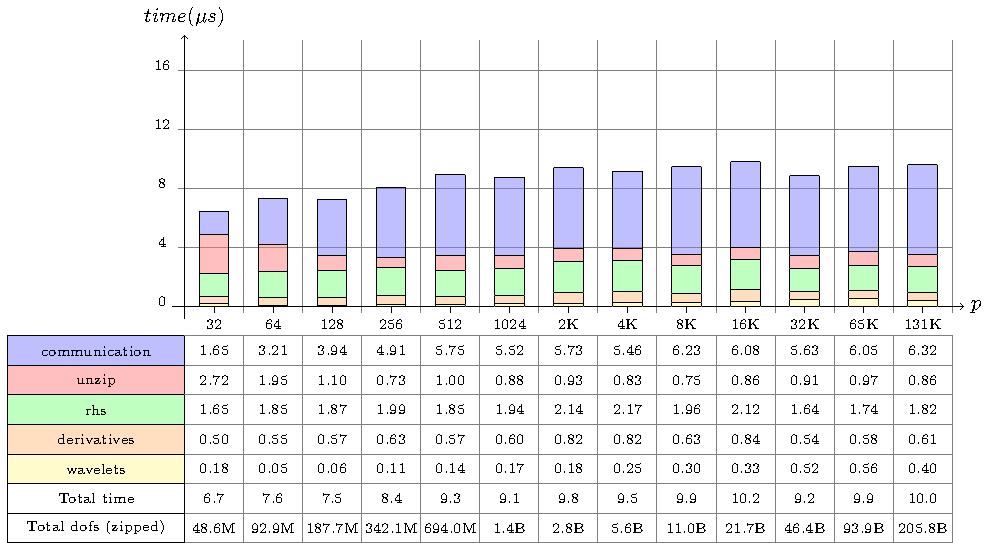
\includegraphics{plots/weak_r10}}}
	%\caption{\small Weak scaling results in ORNL's \Titan~for  $RK/(dof/p)$ (averaged over 10 steps) where $RK,dof,p$ denotes the time for single $RK$ step, degrees of freedom, and number of cores respectively,  with derivative computation (\texttt{deriv}), right hand side( {\texttt rhs}) computation, \texttt{unzip} cost, wavelet computation(\texttt{wavelets}) and communication cost (\texttt{comm}) with the approximate grain size of 1.536M unknowns where the number of cores ranging from $32$ to $131,072$ cores on $8192$ nodes where the largest problem having $206$ Billion unknowns.\label{fig:ws_g1000}}  % Above results are generated with mass ratio $\mu=10$ with \maxDepth~ 18 and wavelet tolerance of $10^{-6}$ 
	\vspace{-0.2in}
\end{figure}	
\vspace{-0.5in}
%Weak scaling results in ORNL's \Titan~for  $RK/(dof/p)$ (averaged over 10 steps) where $RK,dof,p$ denotes the time for single $RK$ step, degrees of freedom, and number of cores respectively,  with derivative computation (\texttt{deriv}), right hand side( {\texttt rhs}) computation, \texttt{unzip} cost, wavelet computation(\texttt{wavelets}) and communication cost (\texttt{comm}) with the approximate grain size of 1.536M unknowns where the number of cores ranging from $32$ to $131,072$ cores on $8192$ nodes where the largest problem having $206$ Billion unknowns.
\end{frame}


\begin{frame}{Strong Scalability on \Titan~ upto $65K$ cores}
\begin{figure}
		\centering
\resizebox{!}{7\TPHorizModule}{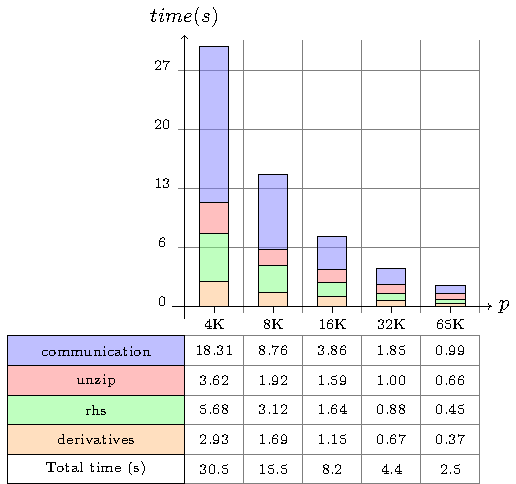
\includegraphics{plots/strong_r10}}
%		\caption{\small Strong scaling results in ORNL's \Titan~for a single RK step (averaged over 10 steps) with derivative computation (\texttt{deriv}), right hand side( {\texttt rhs}) computation, \texttt{unzip} cost and communication cost (\texttt{comm}) for a fixed problem size of $10.5B$ unknowns where the number of cores ranging from $4,096$ to $65,536$ cores on $4096$ nodes. Note that for strong scaling results re-meshing is disabled in order to keep the problem size fixed.  \label{fig:ss_r10} }
\end{figure}	
%Strong scaling results in ORNL's \Titan~for a single RK step (averaged over 10 steps) with derivative computation (\texttt{deriv}), right hand side( {\texttt rhs}) computation, \texttt{unzip} cost and communication cost (\texttt{comm}) for a fixed problem size of $10.5B$ unknowns where the number of cores ranging from $4,096$ to $65,536$ cores on $4096$ nodes. Note that for strong scaling results re-meshing is disabled in order to keep the problem size fixed.
\end{frame}


\begin{frame}{Comparison with Einstein Toolkit(ET)}
\begin{figure}
	\centering
\centering
\resizebox{0.98\textwidth}{!}{
	\begin{tikzpicture}[scale=0.7]
	\begin{axis}[
	ylabel={time per $RK$ step (s) $\rightarrow$},
	% xlabel={number of cores $\rightarrow$},
	legend pos=north west,symbolic x coords={48,96,192,384,768,1536,3072},xtick = data,
	height=3.38in,
	width=3.38in,
	%extra x tick style={tick label style={black, below, yshift=1.5ex}},
	xticklabels=\empty,
	ticklabel style={left}, grid=major, 
	extra x ticks={48,96,192,384,768,1536,3072},
	extra x tick labels={48,96,192,384,768,1536,3072},
	extra x tick style={tick label style={black, below, yshift=0.5ex}},
	legend style={at={(0.5,1.05)},anchor=south},
	%yticklabels=\empty,
	%extra y tick style={yticklabel style={xshift=1cm, anchor=west}}
	]
	\addplot[thick,sq_b1,smooth,mark options={scale=0.8}]  table [x={npes},y ={rkstep}]{dat/stampede2/et_ss_4M.dat};
	\addplot[thick,sq_g1,smooth,mark options={scale=0.8}]  table [x={npes},y ={rkstep}]{dat/stampede2/dendro_ss_4M.dat};
	
	\addplot[thick,sq_b2,opacity=0.6,smooth]  table [x={npes},y ={rkstep_ws_3}]{dat/stampede2/et_ws_2K.dat};
	\addplot[thick,sq_g2,opacity=0.6,smooth]  table [x={npes},y ={rkstep_ws_3}]{dat/stampede2/dendro_ws_2K.dat};
	\legend{\small \ET(strong scaling), \dendrogr(strong scaling), \ET(weak scaling), \dendrogr(weak scaling) }
	
	\end{axis}
	
	\begin{scope}[xshift=-2.5cm]
	% dendro
	%table grid
	\draw (-7,0) grid +(7,7);
	% weak scaling highlight
	\draw[fill=sq_g1, opacity=0.3] (-6-1,0) rectangle +(1,1);
	\draw[fill=sq_g1, opacity=0.3] (-5-1,1) rectangle +(1,1);
	\draw[fill=sq_g1, opacity=0.3] (-4-1,2) rectangle +(1,1);
	\draw[fill=sq_g1, opacity=0.3] (-3-1,3) rectangle +(1,1);
	\draw[fill=sq_g1, opacity=0.3] (-2-1,4) rectangle +(1,1);
	\draw[fill=sq_g1, opacity=0.3] (-1-1,5) rectangle +(1,1);
	\draw[fill=sq_g1, opacity=0.3] (-1,6) rectangle +(1,1);
	
	% strong scaling highlight
	\draw[fill=sq_g1, opacity=0.5, sq_g1] (-6.01-1,3) rectangle +(6.02+1,1);
	
	% data - dendro
	%                 48                                       96                                          192                                           384                                768                                 1536	3072
	\node at (-5.5-1,0.5) {\scriptsize $0.83$}; \node at (-4.5-1,0.5) {\scriptsize $0.55$}; \node at (-3.5-1,0.5) {\scriptsize $0.37$}; \node at (-2.5-1,0.5) {\scriptsize $-$}; \node at (-1.5-1,0.5) {\scriptsize $-$}; \node at (-0.5-1,0.5) {\scriptsize $-$}; \node at (-0.5,0.5) {\scriptsize $-$}; % 500K
	\node at (-5.5-1,1.5) {\scriptsize $1.58$}; \node at (-4.5-1,1.5) {\scriptsize $0.86$}; \node at (-3.5-1,1.5) {\scriptsize $0.51$}; \node at (-2.5-1,1.5) {\scriptsize $0.35$}; \node at (-1.5-1,1.5) {\scriptsize $-$}; \node at (-0.5-1,1.5) {\scriptsize $-$};  \node at (-0.5,1.5) {\scriptsize $-$};% 1M
	\node at (-5.5-1,2.5) {\scriptsize $2.98$}; \node at (-4.5-1,2.5) {\scriptsize $1.57$}; \node at (-3.5-1,2.5) {\scriptsize $0.83$}; \node at (-2.5-1,2.5) {\scriptsize $0.61$}; \node at (-1.5-1,2.5) {\scriptsize $0.38$}; \node at (-0.5-1,2.5) {\scriptsize $-$}; \node at (-0.5,2.5) {\scriptsize $-$};% 2M
	\node at (-5.5-1,3.5) {\scriptsize $5.90$};    \node at (-4.5-1,3.5) {\scriptsize $3.35$}; \node at (-3.5-1,3.5) {\scriptsize $1.75$}; \node at (-2.5-1,3.5) {\scriptsize $1.04$}; \node at (-1.5-1,3.5) {\scriptsize $0.54$}; \node at (-0.5-1,3.5) {\scriptsize $0.39$}; \node at (-0.5,3.5) {\scriptsize $-$}; % 4M
	\node at (-5.5-1,4.5) {\scriptsize $11.23$};    \node at (-4.5-1,4.5) {\scriptsize $6.59$};    \node at (-3.5-1,4.5) {\scriptsize $3.67$}; \node at (-2.5-1,4.5) {\scriptsize $1.92$}; \node at (-1.5-1,4.5) {\scriptsize $1.10$}; \node at (-0.5-1,4.5) {\scriptsize $0.69$}; \node at (-0.5,4.5) {\scriptsize $0.38$};% 8M
	\node at (-5.5-1,5.5) {\scriptsize $19.22$};    \node at (-4.5-1,5.5) {\scriptsize $11.08$};    \node at (-3.5-1,5.5) {\scriptsize $6.22$};    \node at (-2.5-1,5.5) {\scriptsize $3.20$}; \node at (-1.5-1,5.5) {\scriptsize $1.64$}; \node at (-0.5-1,5.5) {\scriptsize $0.98$}; \node at (-0.5,5.5) {\scriptsize $0.56$};% 16M
	\node at (-5.5-1,6.5) {\scriptsize $35.46$};    \node at (-4.5-1,6.5) {\scriptsize $-$};    \node at (-3.5-1,6.5) {\scriptsize $12.34$};    \node at (-2.5-1,6.5) {\scriptsize $6.88$};    \node at (-1.5-1,6.5) {\scriptsize $4.01$}; \node at (-0.5-1,6.5) {\scriptsize $2.06$};  \node at (-0.5,6.5) {\scriptsize $1.06$};% 32M
	
	\node at (-5.5-1,-0.25) {\scriptsize $48$};
	\node at (-4.5-1,-0.25) {\scriptsize $96$};
	\node at (-3.5-1,-0.25) {\scriptsize $192$};
	\node at (-2.5-1,-0.25) {\scriptsize $384$};
	\node at (-1.5-1,-0.25) {\scriptsize $768$};
	\node at (-0.5-1,-0.25) {\scriptsize $1536$};
	\node at (-0.5,-0.25)   {\scriptsize $3072$};
	
	
	\draw[-latex'] (-6.25-1,6.75) -- (-6.25-1,7.25); \node at (-6.75-1, 7) {\scriptsize dofs};  \node at (-6.75-1, 7.35) {\scriptsize total};
	
	\node at (-6.6-1,6.5) {\scriptsize $768M$};
	\node at (-6.6-1,5.5) {\scriptsize $384M$};
	\node at (-6.6-1,4.5) {\scriptsize $192M$};
	\node at (-6.6-1,3.5) {\scriptsize $96M$};
	\node at (-6.6-1,2.5) {\scriptsize $48M$};
	\node at (-6.6-1,1.5) {\scriptsize $24M$};
	\node at (-6.6-1,0.5) {\scriptsize $12M$};
	
	\draw[-latex'] (0,-0.25) -- (0.75,-0.25); \node at (1.0, 0) {\scriptsize cores};
	
	\draw[-latex'] (-1,7.3) -- (-1,7.8);   \node at (0, 7.5) {\scriptsize per core};  \node at (0, 8) {\scriptsize dofs (along the diagonal) };    
	
	\draw[-latex'] (0.25,7.25) -- (-0.25,6.75); \node at (0.75,7) {\scriptsize $250K$};
	\draw[-latex'] (0.25,6.25) -- (-0.25,5.75); \node at (0.75,6) {\scriptsize $125K$};
	\draw[-latex'] (0.25,5.25) -- (-0.25,4.75); \node at (0.75,5) {\scriptsize $62K$};
	\draw[-latex'] (0.25,4.25) -- (-0.25,3.75); \node at (0.75,4) {\scriptsize $31K$};
	\draw[-latex'] (0.25,3.25) -- (-0.25,2.75); \node at (0.75,3) {\scriptsize $15K$};
	\draw[-latex'] (0.25,2.25) -- (-0.25,1.75); \node at (0.75,2) {\scriptsize $8K$};
	\draw[-latex'] (0.25,1.25) -- (-0.25,0.75); \node at (0.75,1) {\scriptsize $4K$};
	
	\node at (-4, 9) {\dendrogr};
	
	
	
	\end{scope}
	
	\begin{scope}[xshift=2.5cm]
	% ET
	% table grid
	\draw (7,0) grid +(7,7);
	% weak highlight 
	\draw[fill=sq_b1, opacity=0.3] (7,0) rectangle +(1,1);
	\draw[fill=sq_b1, opacity=0.3] (8,1) rectangle +(1,1);
	\draw[fill=sq_b1, opacity=0.3] (9,2) rectangle +(1,1);
	\draw[fill=sq_b1, opacity=0.3] (10,3) rectangle +(1,1);
	\draw[fill=sq_b1, opacity=0.3] (11,4) rectangle +(1,1);
	\draw[fill=sq_b1, opacity=0.3] (12,5) rectangle +(1,1);
	\draw[fill=sq_b1, opacity=0.3] (12,5) rectangle +(1,1);
	
	%strong highlights 
	\draw[fill=sq_b1, opacity=0.5, sq_b1] (6.99,3) rectangle +(6.02+1,1);
	
	% data - ET 
	%                 48                                       96                                          192                                           384                                768                                 1536 
	\node at (7.5,0.5) {\scriptsize $2.27$}; \node at (8.5,0.5) {\scriptsize $2.06$}; \node at (9.5,0.5) {\scriptsize $1.93$}; \node at (10.5,0.5) {\scriptsize $1.88$}; \node at (11.5,0.5) {\scriptsize $2.03$}; \node at (12.5,0.5) {\scriptsize $2.07$}; \node at (13.5,0.5) {\scriptsize $-$};% 500K
	\node at (7.5,1.5) {\scriptsize $2.67$}; \node at (8.5,1.5) {\scriptsize $2.31$}; \node at (9.5,1.5) {\scriptsize $2.08$}; \node at (10.5,1.5) {\scriptsize $1.94$}; \node at (11.5,1.5) {\scriptsize $2.07$}; \node at (12.5,1.5) {\scriptsize $2.04$}; \node at (13.5,1.5) {\scriptsize $-$}; % 1M
	\node at (7.5,2.5) {\scriptsize $3.36$}; \node at (8.5,2.5) {\scriptsize $2.68$}; \node at (9.5,2.5) {\scriptsize $2.31$}; \node at (10.5,2.5) {\scriptsize $2.08$}; \node at (11.5,2.5) {\scriptsize $2.12$}; \node at (12.5,2.5) {\scriptsize $2.08$}; \node at (13.5,2.5) {\scriptsize $-$};% 2M
	\node at (7.5,3.5) {\scriptsize $4.68$};    \node at (8.5,3.5) {\scriptsize $3.46$}; \node at (9.5,3.5) {\scriptsize $2.69$}; \node at (10.5,3.5) {\scriptsize $2.32$}; \node at (11.5,3.5) {\scriptsize $3.45$}; \node at (12.5,3.5) {\scriptsize $2.16$}; \node at (13.5,3.5) {\scriptsize $-$}; % 4M
	\node at (7.5,4.5) {\scriptsize $7.13$};    \node at (8.5,4.5) {\scriptsize $4.76$};    \node at (9.5,4.5) {\scriptsize $3.45$}; \node at (10.5,4.5) {\scriptsize $2.74$}; \node at (11.5,4.5) {\scriptsize $2.51$}; \node at (12.5,4.5) {\scriptsize $2.31$}; \node at (13.5,4.5) {\scriptsize $-$}; % 8M
	\node at (7.5,5.5) {\scriptsize $12.44$};    \node at (8.5,5.5) {\scriptsize $7.51$};    \node at (9.5,5.5) {\scriptsize $4.87$};    \node at (10.5,5.5) {\scriptsize $3.48$}; \node at (11.5,5.5) {\scriptsize $2.92$}; \node at (12.5,5.5) {\scriptsize $2.52$}; \node at (13.5,5.5) {\scriptsize $-$};% 16M
	\node at (7.5,6.5) {\scriptsize $23.38$};    \node at (8.5,6.5) {\scriptsize $12.65$};    \node at (9.5,6.5) {\scriptsize $7.64$};    \node at (10.5,6.5) {\scriptsize $4.93$};    \node at (11.5,6.5) {\scriptsize $3.71$}; \node at (12.5,6.5) {\scriptsize $2.95$}; \node at (13.5,6.5) {\scriptsize $-$};% 32M    
	
	\node at (7.5,-0.25) {\scriptsize $48$};
	\node at (8.5,-0.25) {\scriptsize $96$};
	\node at (9.5,-0.25) {\scriptsize $192$};
	\node at (10.5,-0.25) {\scriptsize $384$};
	\node at (11.5,-0.25) {\scriptsize $768$};
	\node at (12.5,-0.25) {\scriptsize $1536$};
	\node at (13.5,-0.25) {\scriptsize $3072$};
	
	\draw[-latex'] (13+1,-0.25) -- (14+1,-0.25); \node at (13.5+1, 0) {\scriptsize cores};
	
	\draw[-latex'] (6.75,6.75) -- (6.75,7.25); \node at (6.25, 7) {\scriptsize dofs};  \node at (6.25, 7.35) {\scriptsize total};
	
	\node at (7.25-1,6.5) {\scriptsize $768M$};
	\node at (7.25-1,5.5) {\scriptsize $384M$};
	\node at (7.25-1,4.5) {\scriptsize $192M$};
	\node at (7.25-1,3.5) {\scriptsize $96M$};
	\node at (7.25-1,2.5) {\scriptsize $48M$};
	\node at (7.25-1,1.5) {\scriptsize $24M$};
	\node at (7.25-1,0.5) {\scriptsize $12M$};
	
	
	\draw[-latex'] (14,7.3) -- (14,7.8);   \node at (13+2.25, 7.5) {\scriptsize per core};  \node at (13+2.25, 8) {\scriptsize dofs (along the diagonal) };    
	%\node at (13.4, 7) {\scriptsize size};  \node at (13.5, 7.35) {\scriptsize grain};
	
	\draw[-latex'] (13.25+1,7.25) -- (12.75+1,6.75); \node at (13.75+1,7) {\scriptsize $250K$};
	\draw[-latex'] (13.25+1,6.25) -- (12.75+1,5.75); \node at (13.75+1,6) {\scriptsize $125K$};
	\draw[-latex'] (13.25+1,5.25) -- (12.75+1,4.75); \node at (13.75+1,5) {\scriptsize $62K$};
	\draw[-latex'] (13.25+1,4.25) -- (12.75+1,3.75); \node at (13.75+1,4) {\scriptsize $31K$};
	\draw[-latex'] (13.25+1,3.25) -- (12.75+1,2.75); \node at (13.75+1,3) {\scriptsize $15K$};
	\draw[-latex'] (13.25+1,2.25) -- (12.75+1,1.75); \node at (13.75+1,2) {\scriptsize $8K$};
	\draw[-latex'] (13.25+1,1.25) -- (12.75+1,0.75); \node at (13.75+1,1) {\scriptsize $4K$};
	
	\node at (11, 9) {\ET};
	
	
	\end{scope}
	
	
	
	
	
	% table 
	
	
	
	% axis
	%\node at (axis cs:64,11) [anchor=north west] {\tiny $48M$};
	
	
	
	
	
	
	
	
	
	
	
	
	
	\end{tikzpicture}
}
%		\caption{ \tiny Comparison between \ET~ and \dendrogr\ without factoring in adaptivity (i.e. both \ET~ \& \dendrogr~ support uniform grids.). For a fixed tolerance, we expand the domain for a $1:1$ mass-ratio simulation such that both \ET~ and \dendrogr\ have roughly the same number of dofs. We present both weak and strong scaling results using both codes. On the left table are results from \dendrogr\ and from \ET\  on the right. In the middle, we plot a representative strong and weak scaling curve for each code. The \dendrogr\  scaling is plotted in green (lighter shade for weak) and blue for \ET. The corresponding data entries are also marked in the tables. Note that the rows represent strong scaling and the diagonal entries represent weak scaling results and runtime is reported in seconds$(s)$. }
%	\vspace{-0.2in}
\end{figure}
\end{frame}

\begin{frame}{Equal mass ratio binary merger}


\fboxsep=0pt
\fboxrule=0pt
\noindent\fbox{%
	\begin{minipage}[t]{0.48\linewidth}
		\includemovie[autoplay=true,poster,controls=true,toolbar=true]{0.9\textwidth}{0.9\textwidth}{vid/bssn_r1_chi.mp4}
\end{minipage}}%
\hfill%
\fbox{%
	\begin{minipage}[t]{0.48\linewidth}
		\includemovie[autoplay=true,poster,controls=true,toolbar=true]{0.9\textwidth}{0.9\textwidth}{vid/bssn_r1_chi_wf.mp4}	
	\end{minipage}
}

%\begin{figure}
%\begin{minipage}[t]{0.5\textwidth}
%
%\end{minipage} \hfill
%\begin{minipage}[t]{0.5\textwidth}
%\includemovie[autoplay,poster,controls=true,toolbar=true]{0.9\textwidth}{0.9\textwidth}{vid/bssn_r1_chi_wf.mp4}	
%\end{minipage}


%\end{figure}

\end{frame}


\begin{frame}{$\psi_4$ (left $Img(\psi_4)$ and on the right $Re(\psi_4)$) }

\fboxsep=0pt
\fboxrule=0pt
\noindent\fbox{%
\begin{minipage}[t]{0.48\linewidth}
	\includemovie[autoplay=true,poster,controls=true,toolbar=true]{0.9\textwidth}{0.9\textwidth}{vid/bssn_r1_Img_psi4.mp4}
\end{minipage}}%
\hfill%
\fbox{%
\begin{minipage}[t]{0.48\linewidth}
	\includemovie[autoplay=true,poster,controls=true,toolbar=true]{0.9\textwidth}{0.9\textwidth}{vid/bssn_r1_Re_psi4.mp4}	
\end{minipage}
}

\end{frame}



\begin{frame}{Equal mass ratio binary merger}
\begin{figure}
\centering
\begin{tikzpicture}
\begin{axis}[legend pos=north east,xlabel={$time step \rightarrow$},xmin=0,
ylabel={$Y^2_0$ $\rightarrow$},grid=major,width=12cm,height=6cm]
\addplot [blue,thin,smooth]table [x={TimeStep},y={rxpsi_real_lm}]{dat/bssn_prof_GW_50.dat};
\addplot [red,thin,smooth]table [x={TimeStep},y={rxpsi_img_lm}]{dat/bssn_prof_GW_50.dat};
\legend{$Y^2_0(Re(\psi_4))$, $Y^2_0(Im(\psi_4))$}
\end{axis}
\end{tikzpicture}
\caption{Extracted spin($s=-2$) weighted spherical harmonics at $r=50$}
\label{fig::psi_4}

\end{figure}
\end{frame}



\begin{frame}{Conclusion}
	\begin{itemize}
		\item Numerical simulations are essential for gravitational wave extraction can be used to make semi-approximate methods. 
		\item We present fully adaptive scalable framework \dendrogr~ which is able to handle large mass ratios. 
		\item Symbolic code generation makes your framework portable across different architectures
	\end{itemize}
\end{frame}


\begin{frame}
\begin{center}
	\Huge Thank You. 
\end{center}
	
\end{frame}


\begin{frame}
\begin{center}
	\Huge Questions ?
\end{center}

\end{frame}
	
\end{document}

